\newpage

\section{Results and discussion}
\label{Sec:Results}

In this section, the results for the \pT-dependent non-linear flow modes $v_{4,22}$, $v_{5,32}$, $v_{6,33}$ and $v_{6,222}$ of identified particles are presented for various centrality intervals in Pb--Pb collisions at \sNN. We first present the centrality and \pT~dependence of $v_{n,mk}$ in Sec. \ref{SubSec:pTdependence}. The scaling properties of non-linear flow modes are also discussed in this section. Comparisons to two model calculations are shown in Sec. \ref{SubSec:hydro}. Note that the same data are used in different representations to highlight the physics implications of the measurements in each section. 
%~for 0-5\% up to 50-60\% centrality intervals for \pion, \kaon, \proton, \Ks, \lambdas~and $\phi$-meson

\subsection{Centrality and \pT~dependence of non-linear flow modes}
\label{SubSec:pTdependence}

Higher order flow coefficients ($n>3$) are mainly generated by inhomogeneities in the initial density profile, the collision geometry as well as the non-linear hydrodynamic response of the system. Figure \ref{v422_centralityDependence} presents the non-linear term for the fourth order flow coefficient, i.e. $v_{4,22}(p_{\rm{T}})$, of \pion, \kaon, \proton, \lambdas, \Ks~and $\phi$-meson for a wide range of centrality intervals, i.e. 0-60\%. For the $\phi$-meson, the results are reported in the 10-50\% centrality interval, where $v_{4,22}$ can be measured accurately. The magnitude of $v_{4,22}$ rises steeply with increasing centrality interval from 0-5\% to 40-50\% for all particle species. This increase is expected as $v_{4,22}$ measures the contribution of the second order eccentricity, $\varepsilon_{2}$, in $v_{4}$ which increases for peripheral collisions \cite{Alver:2010gr}. For more peripheral collisions (i.e. 50-60\%) , the magnitude of $v_{4,22}$ is smaller than in the previous centrality intervals for all particle species. This effect that was observed also in $v_n$ measurements is probably due to the shorter lifetime of the produced system in more peripheral collisions, which prevents $v_{4,22}$ from developing further. 


\begin{figure}[!htb]
\begin{center}
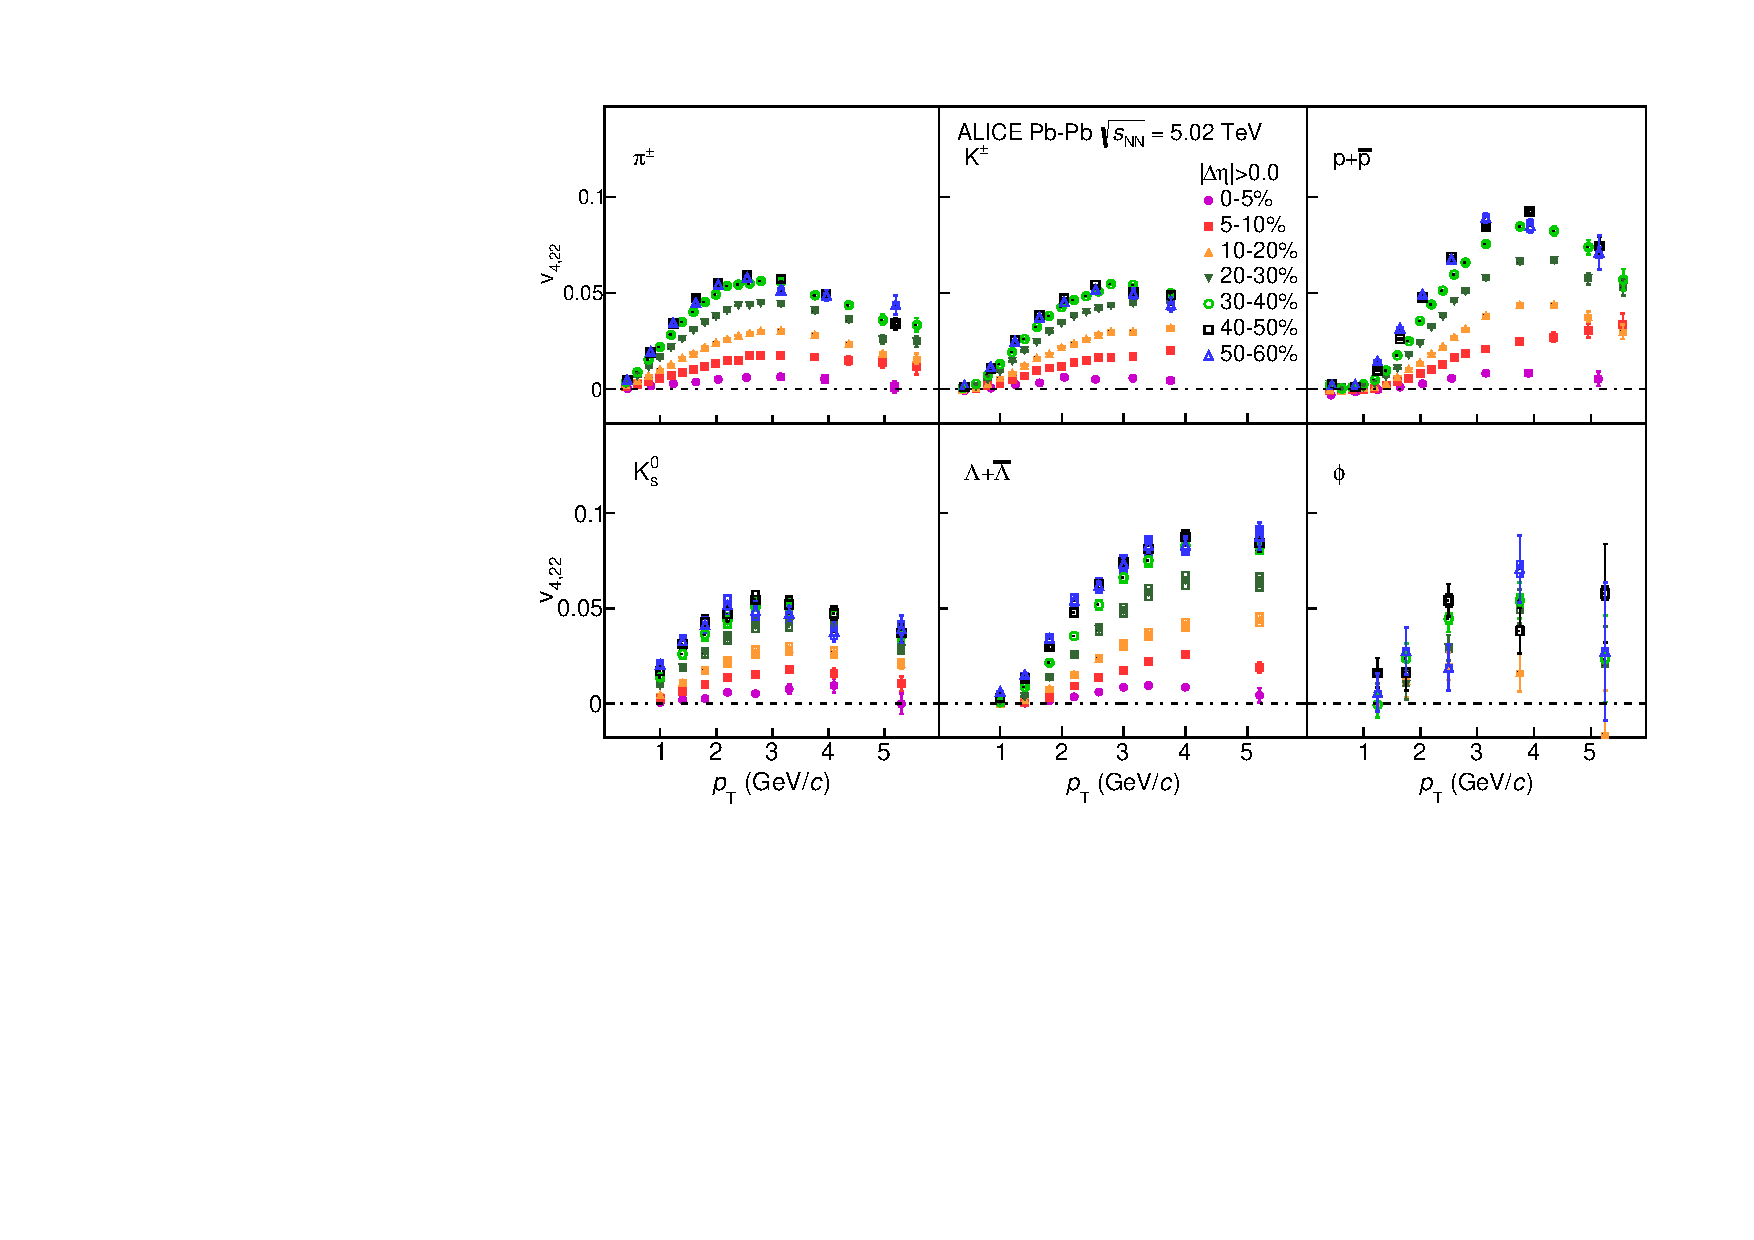
\includegraphics[scale=0.82]{figures/results/All_v422_gap00_CentDep_PID2.pdf}
\end{center}
\caption{The \pT-differential $v_{4,22}$ for different centrality intervals of Pb--Pb collisions at \sNN~ grouped by particle species.}
\label{v422_centralityDependence}
\end{figure}
 
Figure \ref{v523_centralityDependence} presents the non-linear term for the fifth order flow coefficient, i.e. $v_{5,32}(p_{\rm{T}})$, of \pion, \kaon, \proton, \lambdas~and \Ks~for the same range of centrality intervals, i.e. 0-60\%. Statistical precision limits extending the measurements of non-linear flow modes of $\phi$-meson for $n>4$. The measurements show a significant increase in the magnitude of this non-linear flow mode with increasing centrality percentile. This is due to the fact that $v_{5,32}(p_{\rm{T}})$ has a contribution from both $\varepsilon_{2}$ and $\varepsilon_{3}$. It is shown in MC studies that both $\varepsilon_{2}$ and $\varepsilon_{3}$ increase for peripheral collisions \cite{Alver:2010gr}. Although, this increase is less pronounced for $\varepsilon_{3}$.

\begin{figure}[!htb]
\begin{center}
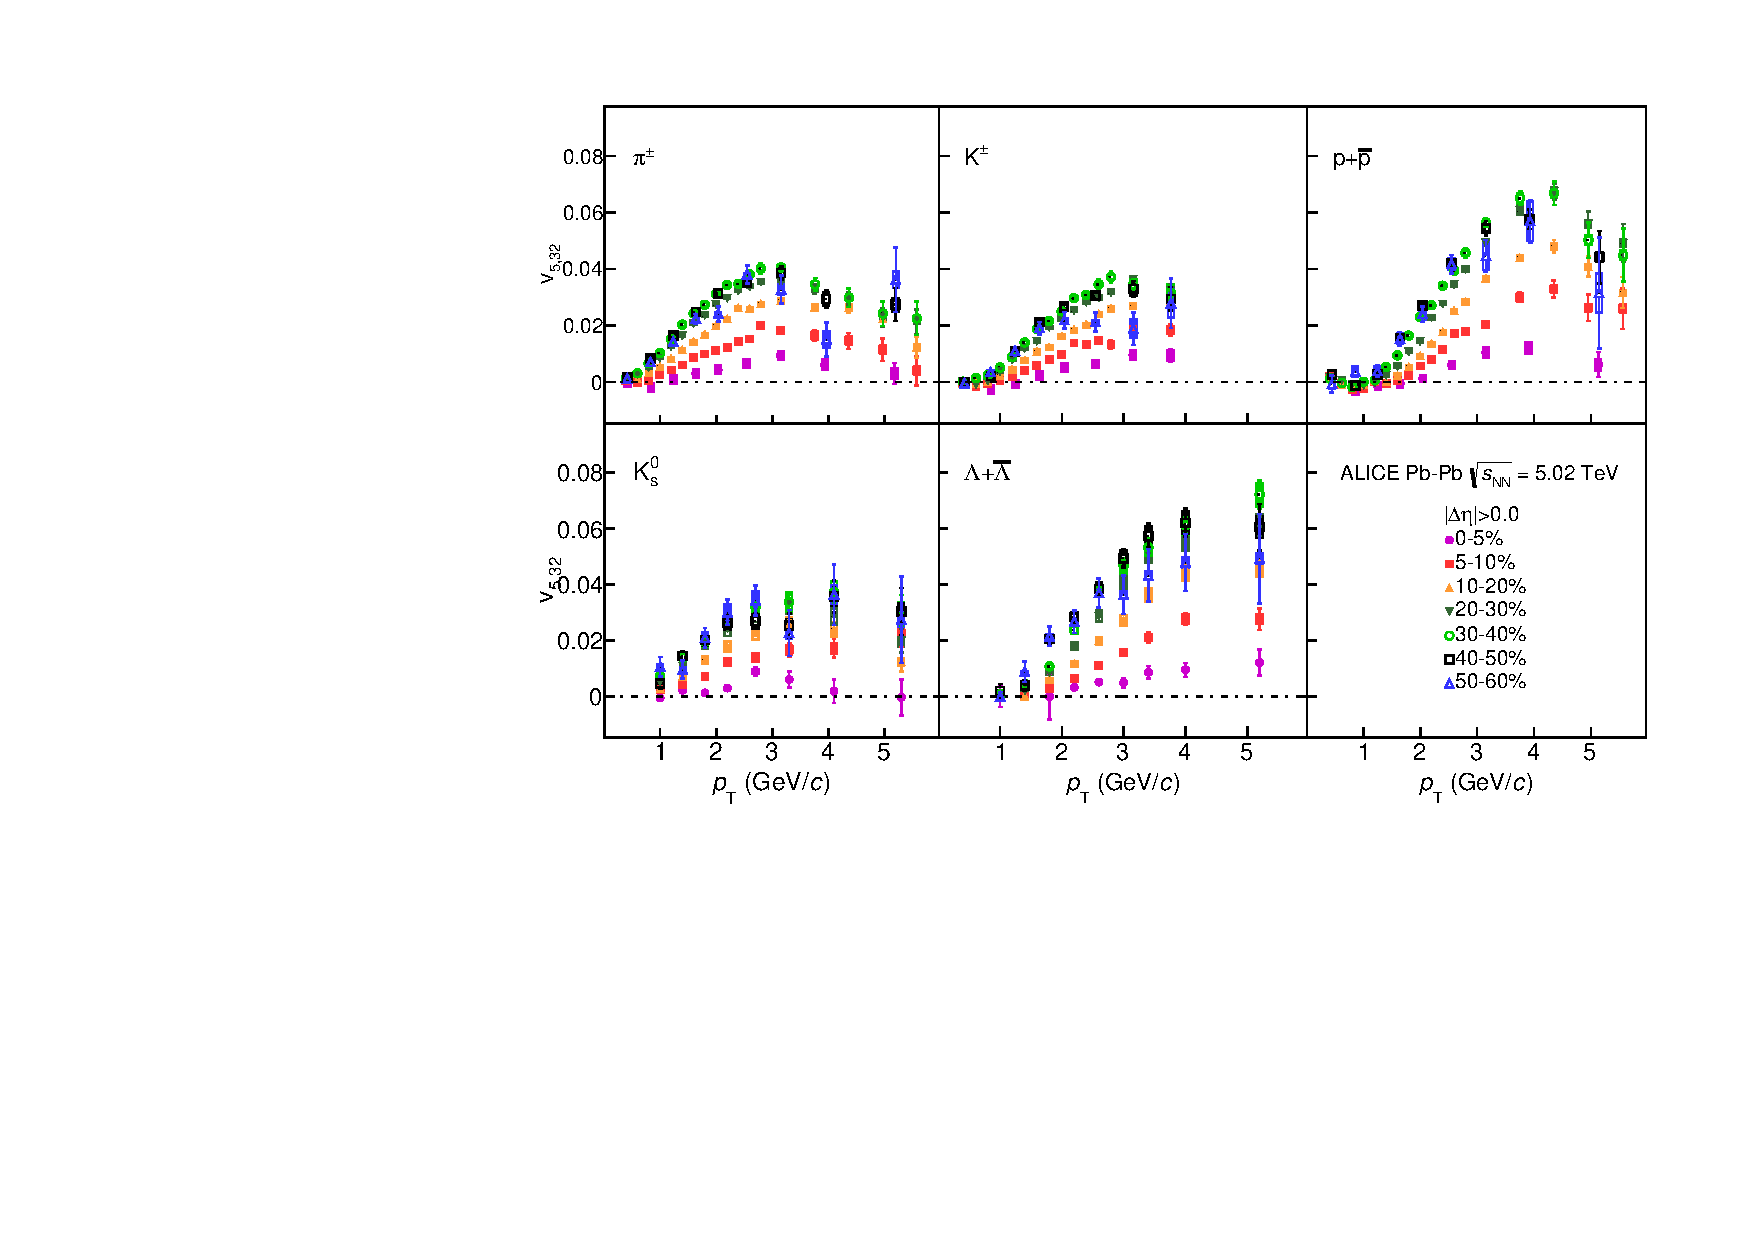
\includegraphics[scale=0.82]{figures/results/All_v523_gap00_CentDep_PID2.pdf}
\end{center}
\caption{The \pT-differential $v_{5,32}$ for different centrality intervals of Pb--Pb collisions at \sNN~ grouped by particle species.}
\label{v523_centralityDependence}
\end{figure}

Figure \ref{v633_centralityDependence} and \ref{v6222_centralityDependence} present the non-linear terms for the sixth order flow coefficient, i.e. $v_{6,33}(p_{\rm{T}})$ for \pion, \kaon, \proton, \lambdas~and \Ks~at 0-50\% centrality intervals and $v_{6,222}(p_{\rm{T}})$ for \pion, \kaon, \proton~at 0-60\% centrality intervals. As expected, measurements of $v_{6,222}(p_{\rm{T}})$ show an increase in the magnitude of this non-linear flow mode with increasing centrality percentile, whereas, $v_{6,33}(p_{\rm{T}})$ presents little to no dependence on centrality. 

\begin{figure}[!htb]
\begin{center}
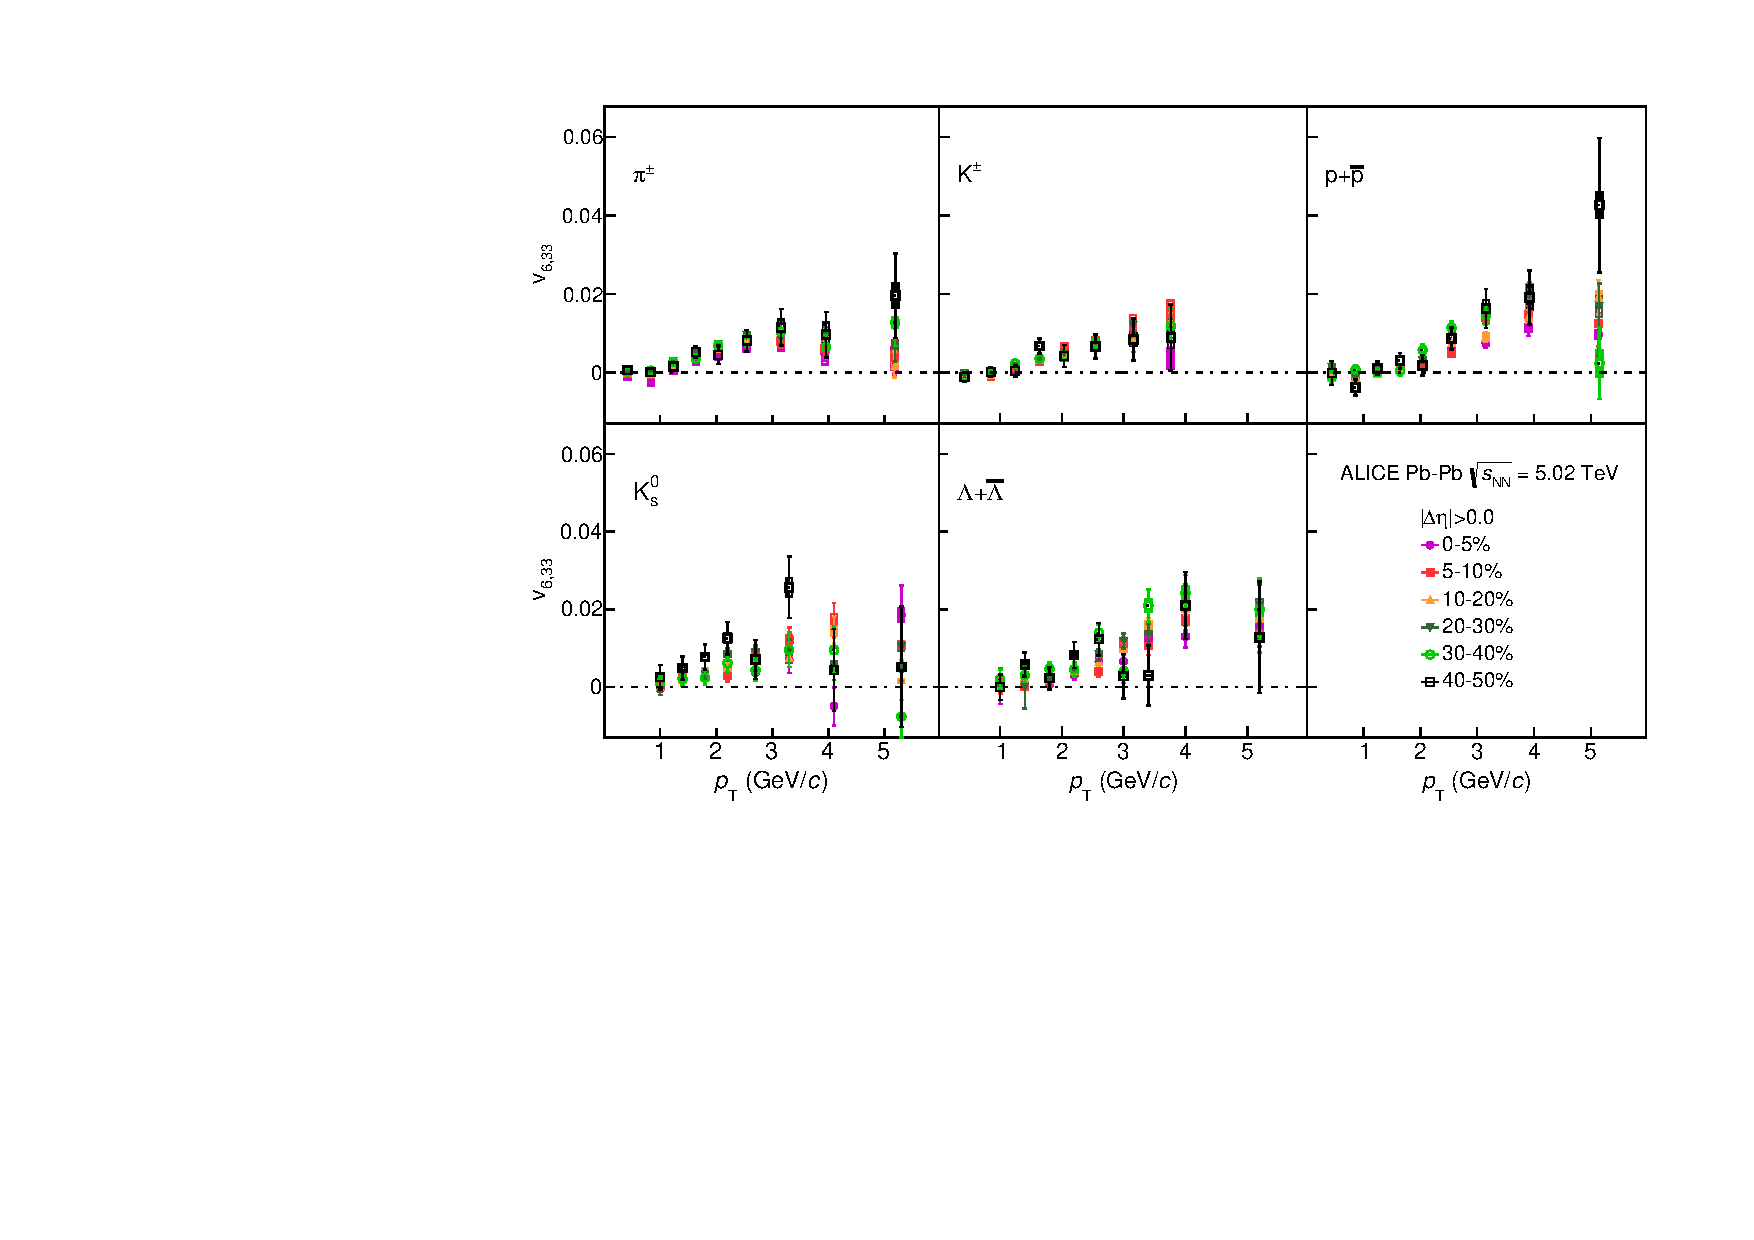
\includegraphics[scale=0.82]{figures/results/All_v633_gap00_CentDep_PID2.pdf}
\end{center}
\caption{The \pT-differential $v_{6,33}$ for different centrality intervals of Pb--Pb collisions at \sNN~ grouped by particle species.}
\label{v633_centralityDependence}
\end{figure}

\begin{figure}[!htb]
\begin{center}
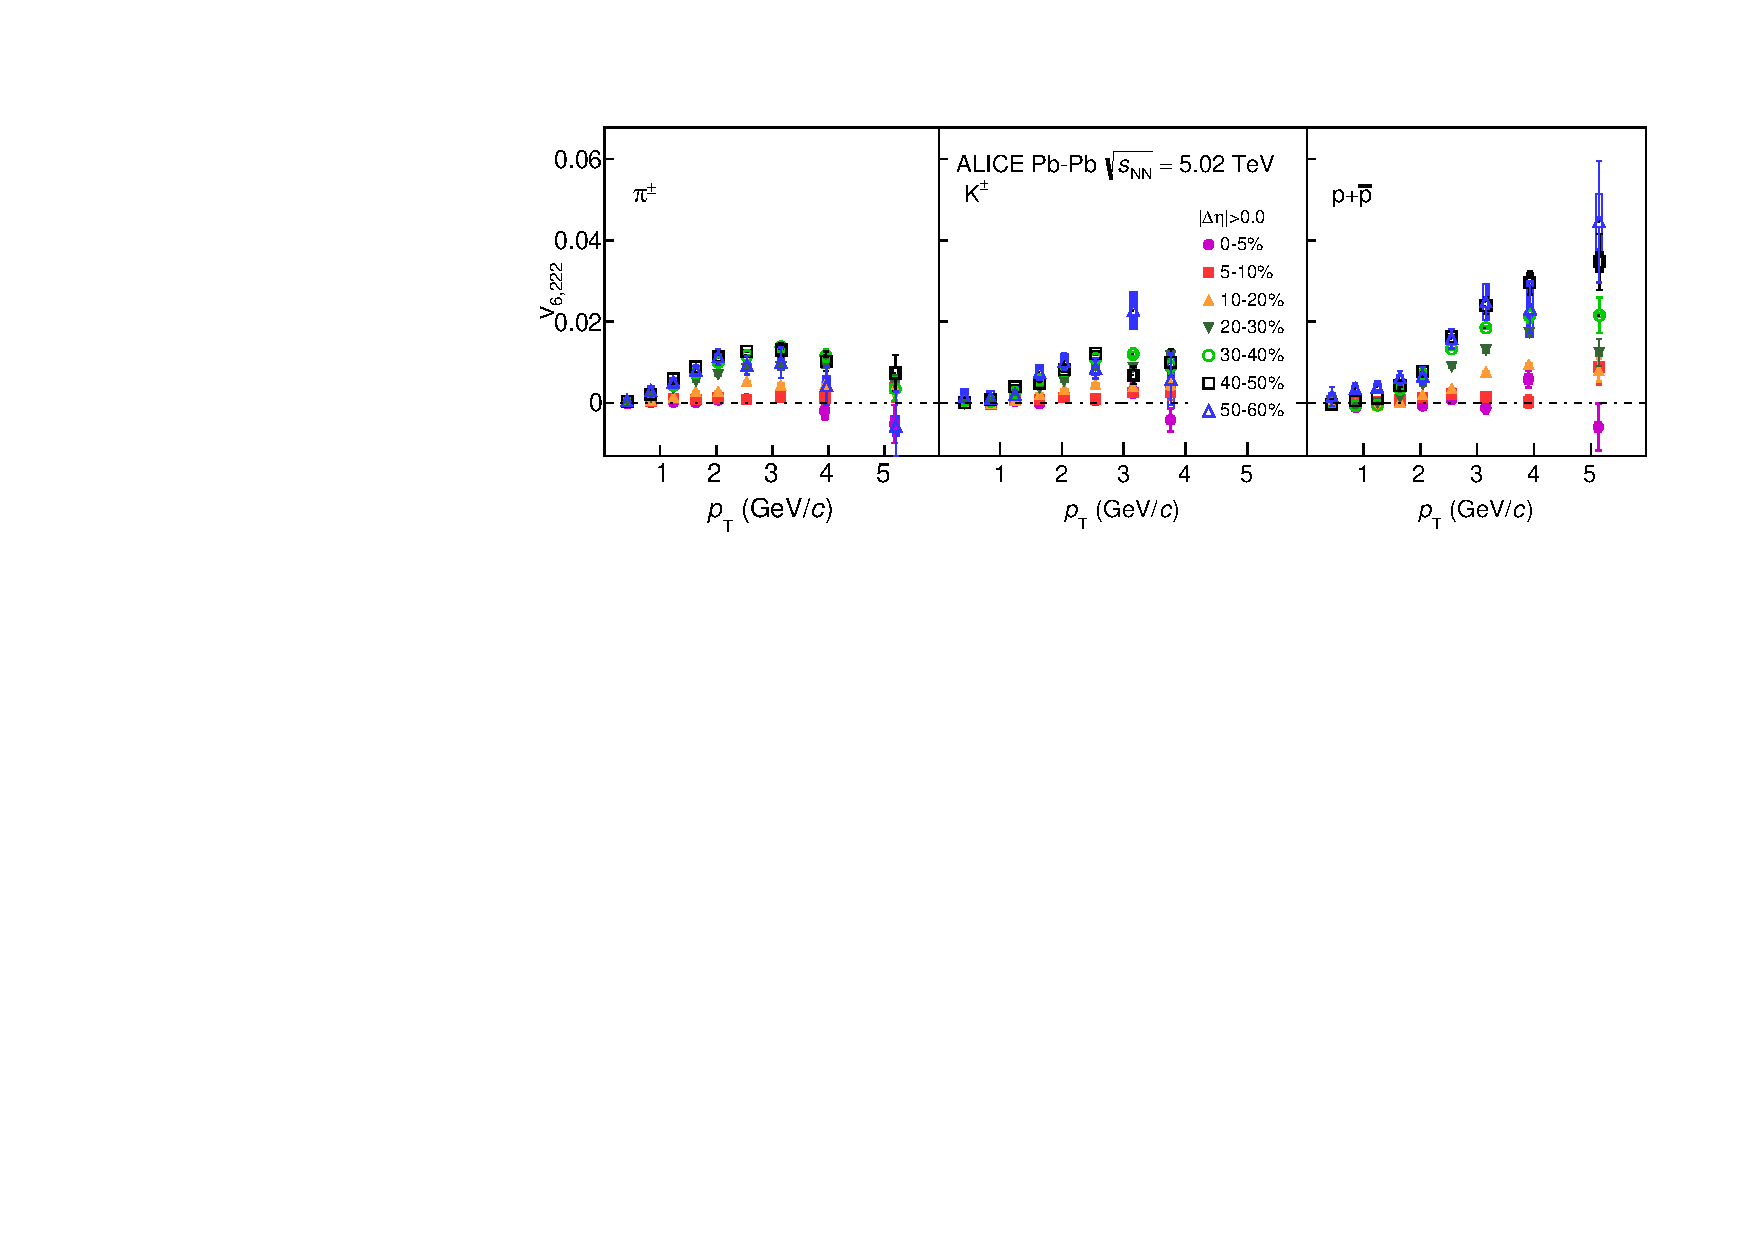
\includegraphics[scale=0.82]{figures/results/All_v6222_gap00_CentDep_PID2.pdf}
\end{center}
\caption{The \pT-differential $v_{6,222}$ for different centrality intervals of Pb--Pb collisions at \sNN~ grouped by particle species.}
\label{v6222_centralityDependence}
\end{figure}

\newpage
%\subsection{Mass ordering}
%\label{MassOrdering}

In Fig. \ref{v422_particleDependence} the same data points are grouped by centrality interval to highlight how $v_{4,22}$ develops for a given centrality for various particle species as a function of \pT.
%Figures \ref{v422_particleDependence} presents the \pT-differential $v_{4,22}$ for \pion, \kaon, \proton, \Ks, \lambdas~and $\phi$-meson starting from most central collisions (0-5\%) up to the 50-60\% centrality interval. 
A clear mass ordering can be seen in the low \pT~region (i.e. \pT $< 2.5$ \GeV) at all collision centralities. This mass dependence arises from the interplay between the anisotropic flow and radial flow. Radial flow creates a depletion in the particle spectra at lower \pT~values which leads to lower $v_{4,22}$ for heavier particles \cite{Shen:2011eg}.


\begin{figure}[!htb]
\begin{center}
%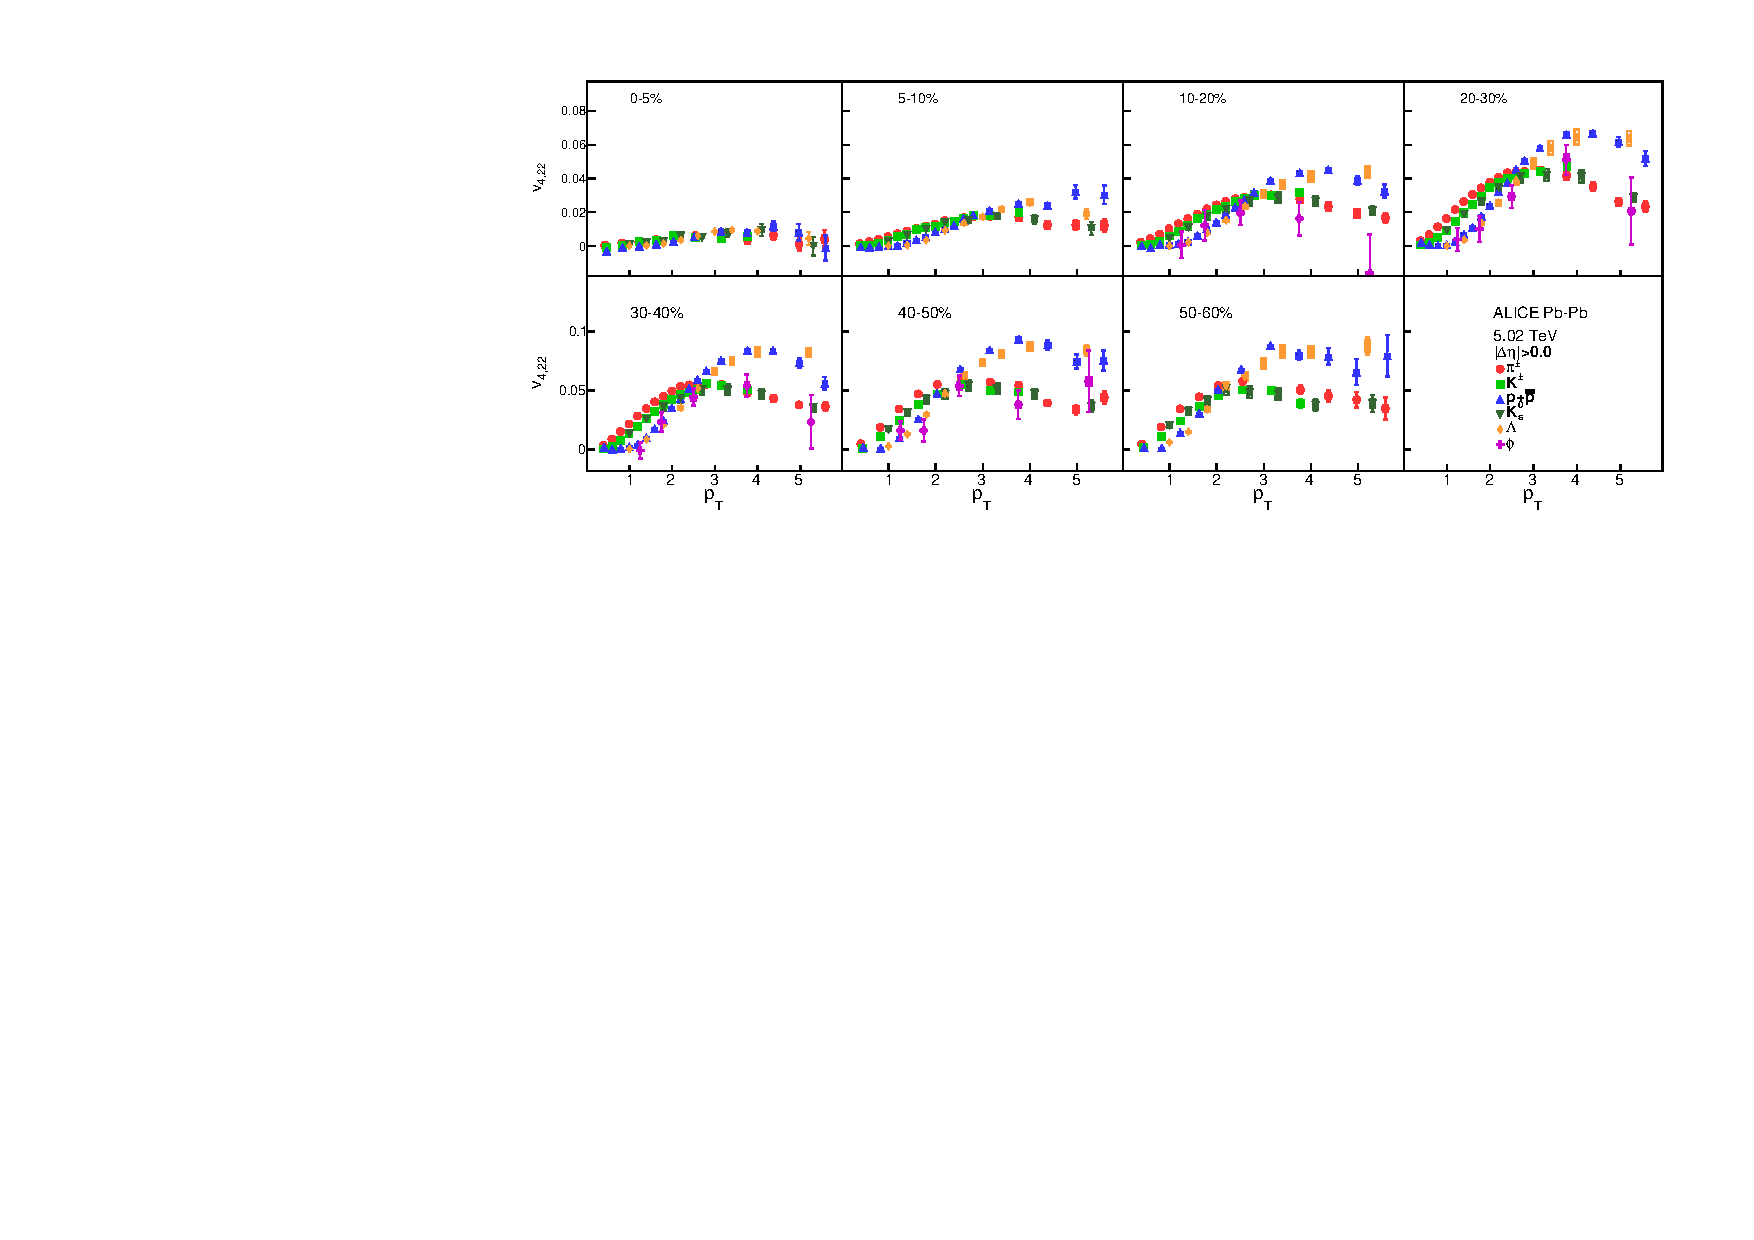
\includegraphics[scale=0.82]{figures/results/All_v422_gap00.pdf}
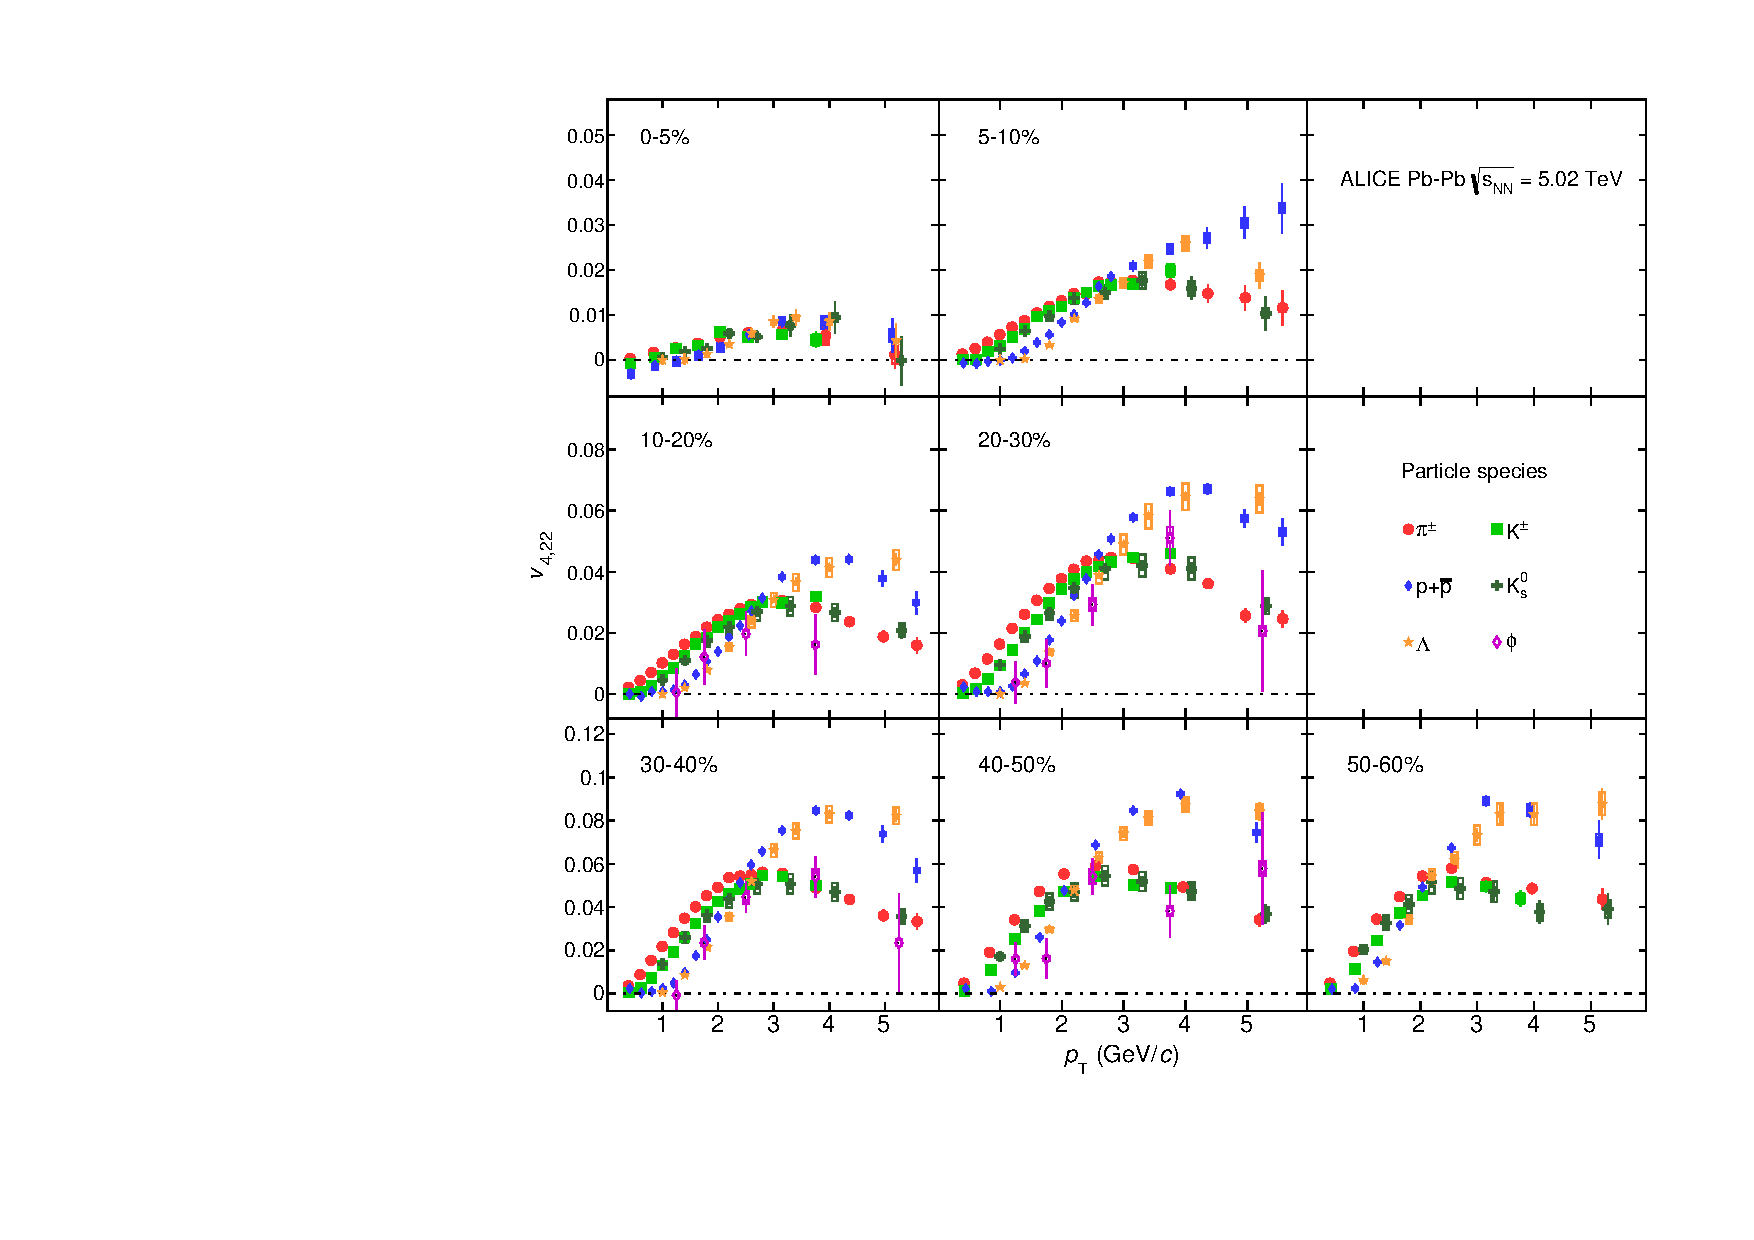
\includegraphics[scale=0.82]{figures/results/All_v422_gap00_PID2_3by3.pdf}
\end{center}
\caption{The \pT-differential $v_{4,22}$ for different particle species grouped into different centrality intervals of Pb--Pb collisions \sNN}
\label{v422_particleDependence}
\end{figure}

Similarly, Figs. \ref{v523_particleDependence}, \ref{v633_particleDependence} and \ref{v6222_particleDependence} show the \pT-differential $v_{5,32}$, $v_{6,33}$ and $v_{6,222}$ respectively, of different particle species for each centrality interval. A clear mass ordering is seen in the low \pT~region, (i.e. \pT $< 2.5$ \GeV), for $v_{5,32}(p_{\rm{T}})$, $v_{6,33}(p_{\rm{T}})$ and $v_{6,222}(p_{\rm{T}})$, which similarly arises from the interplay between the non-linear response of the system and radial flow. 

\begin{figure}[!htb]
\begin{center}
%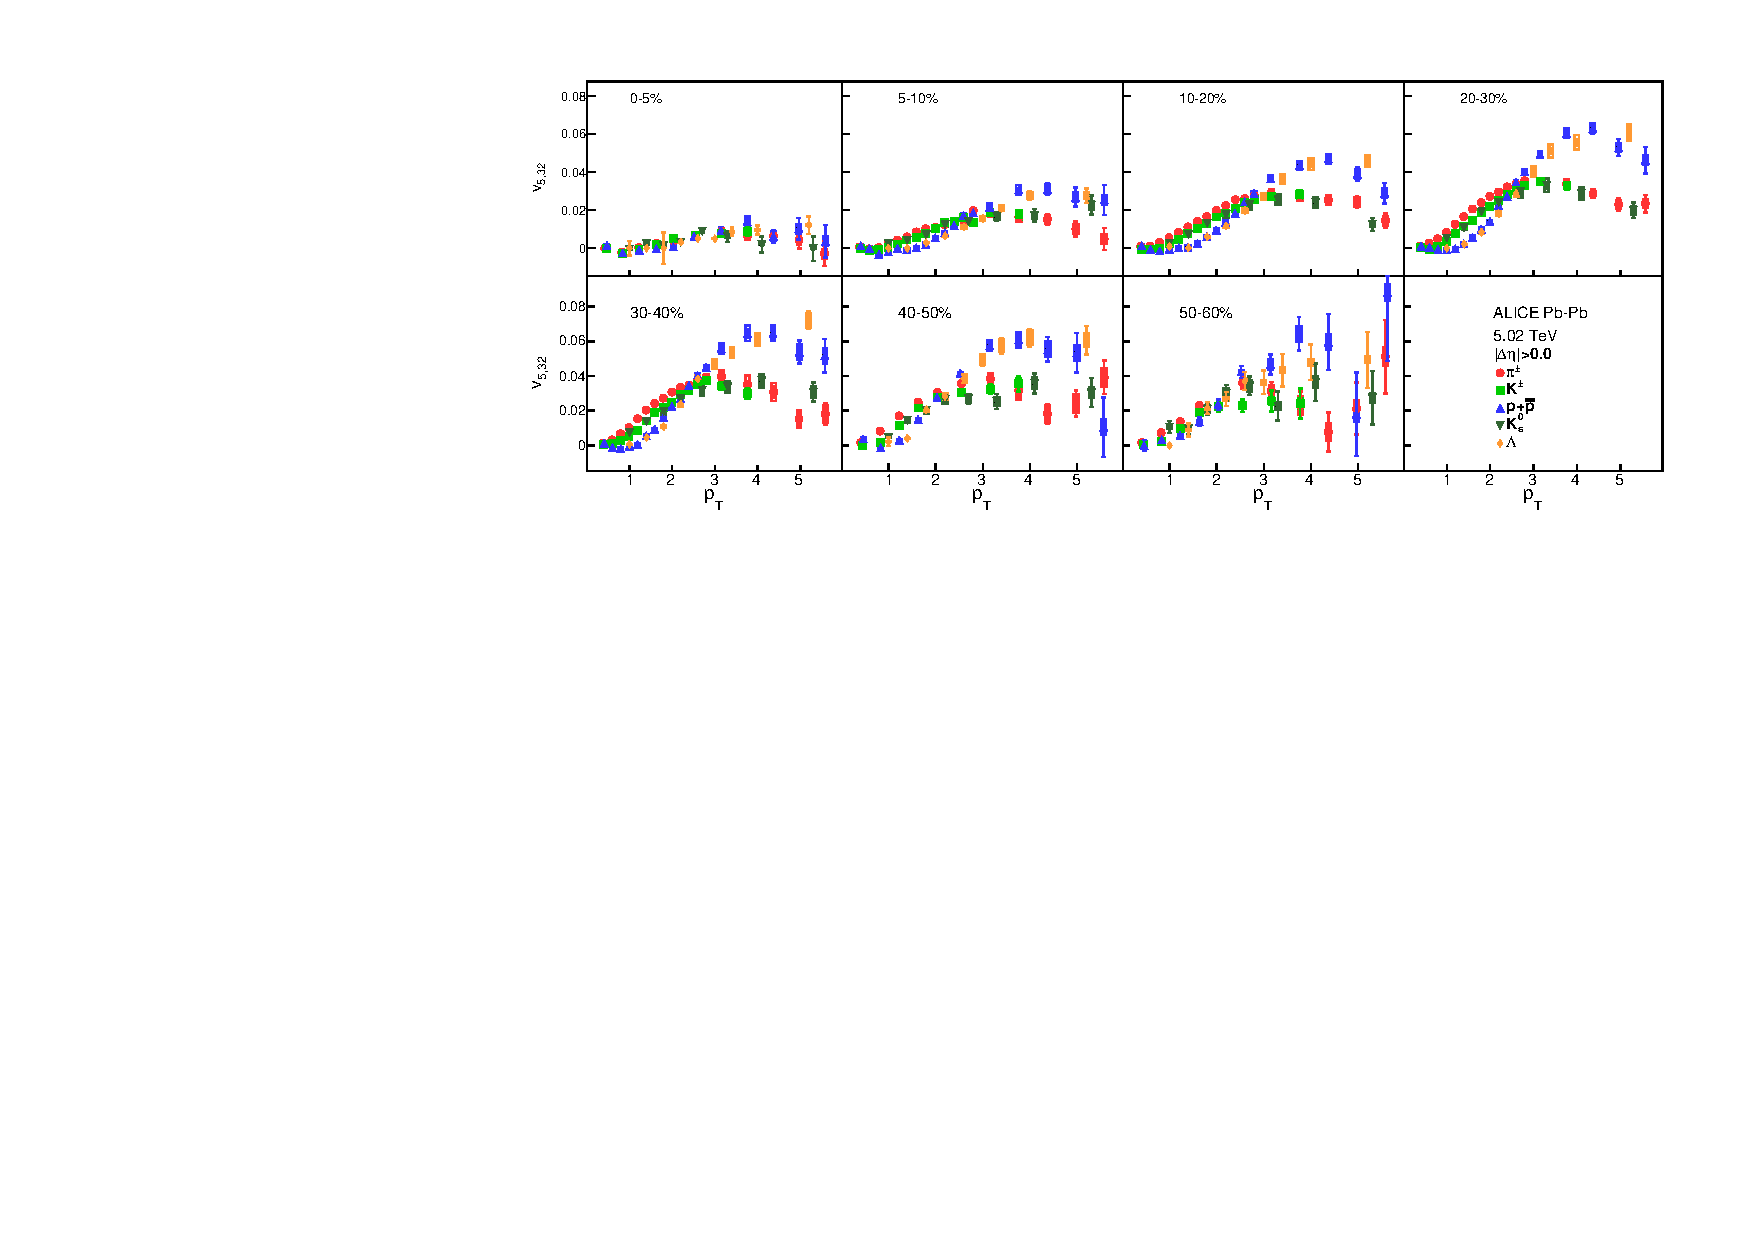
\includegraphics[scale=0.82]{figures/results/All_v523_gap00.pdf}
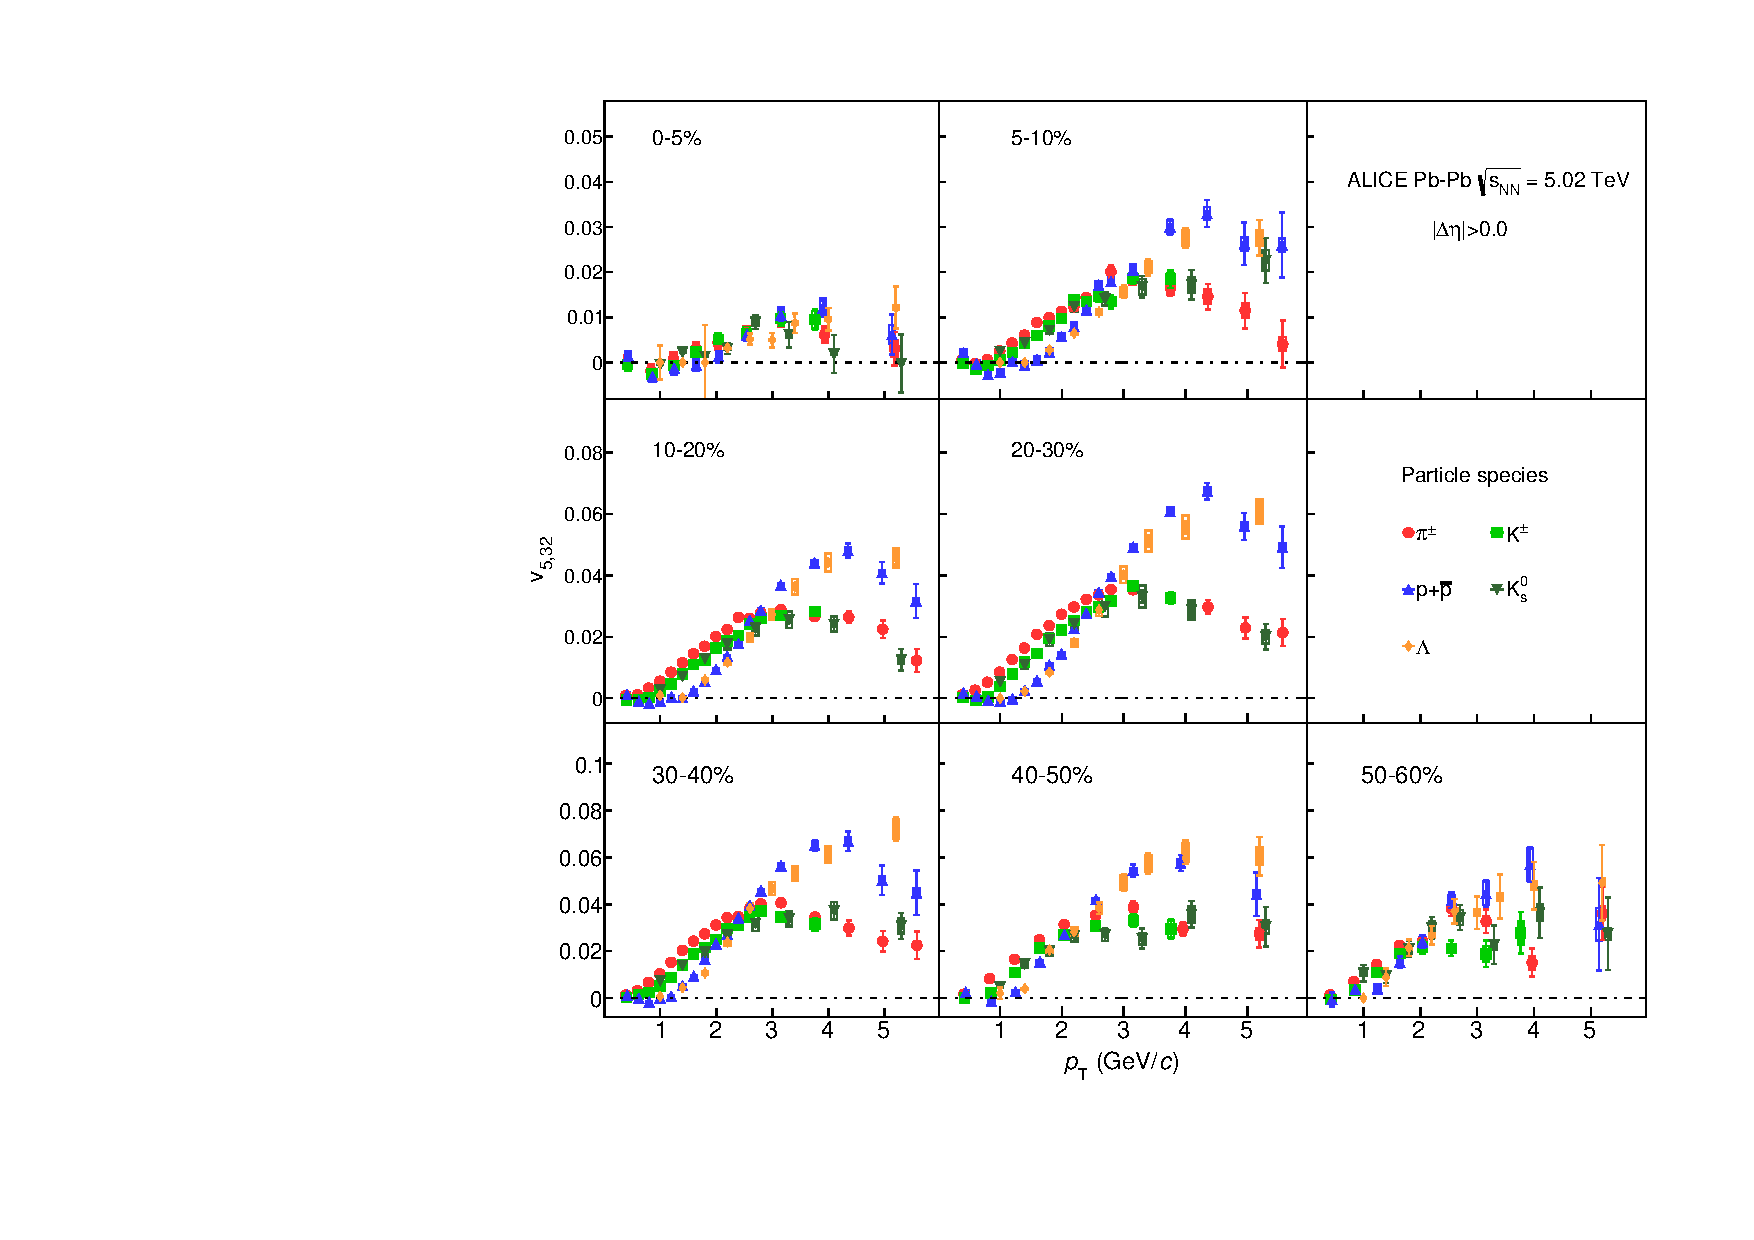
\includegraphics[scale=0.82]{figures/results/All_v523_gap00_PID2_3by3.pdf}

\end{center}
\caption{The \pT-differential $v_{5,32}$ for different particle species grouped into different centrality intervals of Pb--Pb collisions \sNN}
\label{v523_particleDependence}
\end{figure}

\begin{figure}[!htb]
\begin{center}
%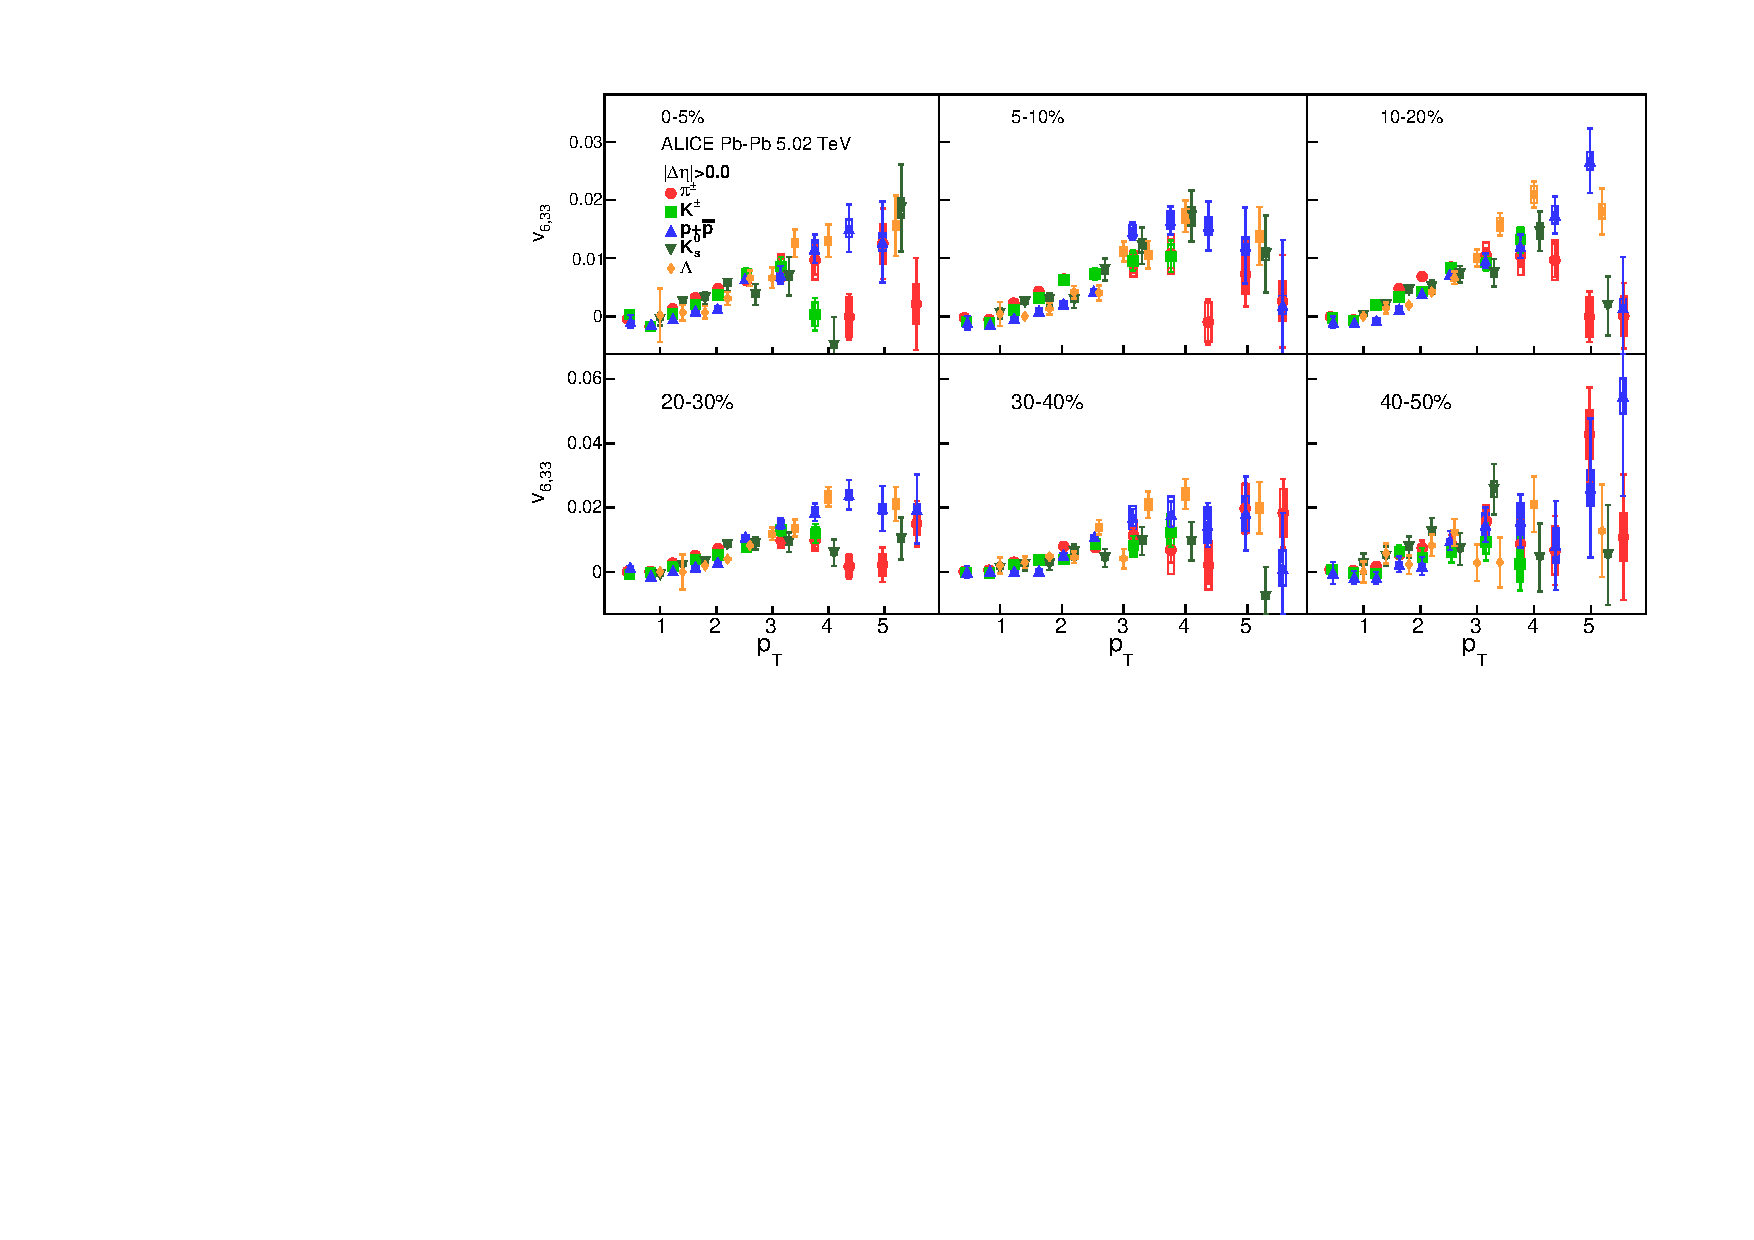
\includegraphics[scale=0.62]{figures/results/All_v633_gap00.pdf}
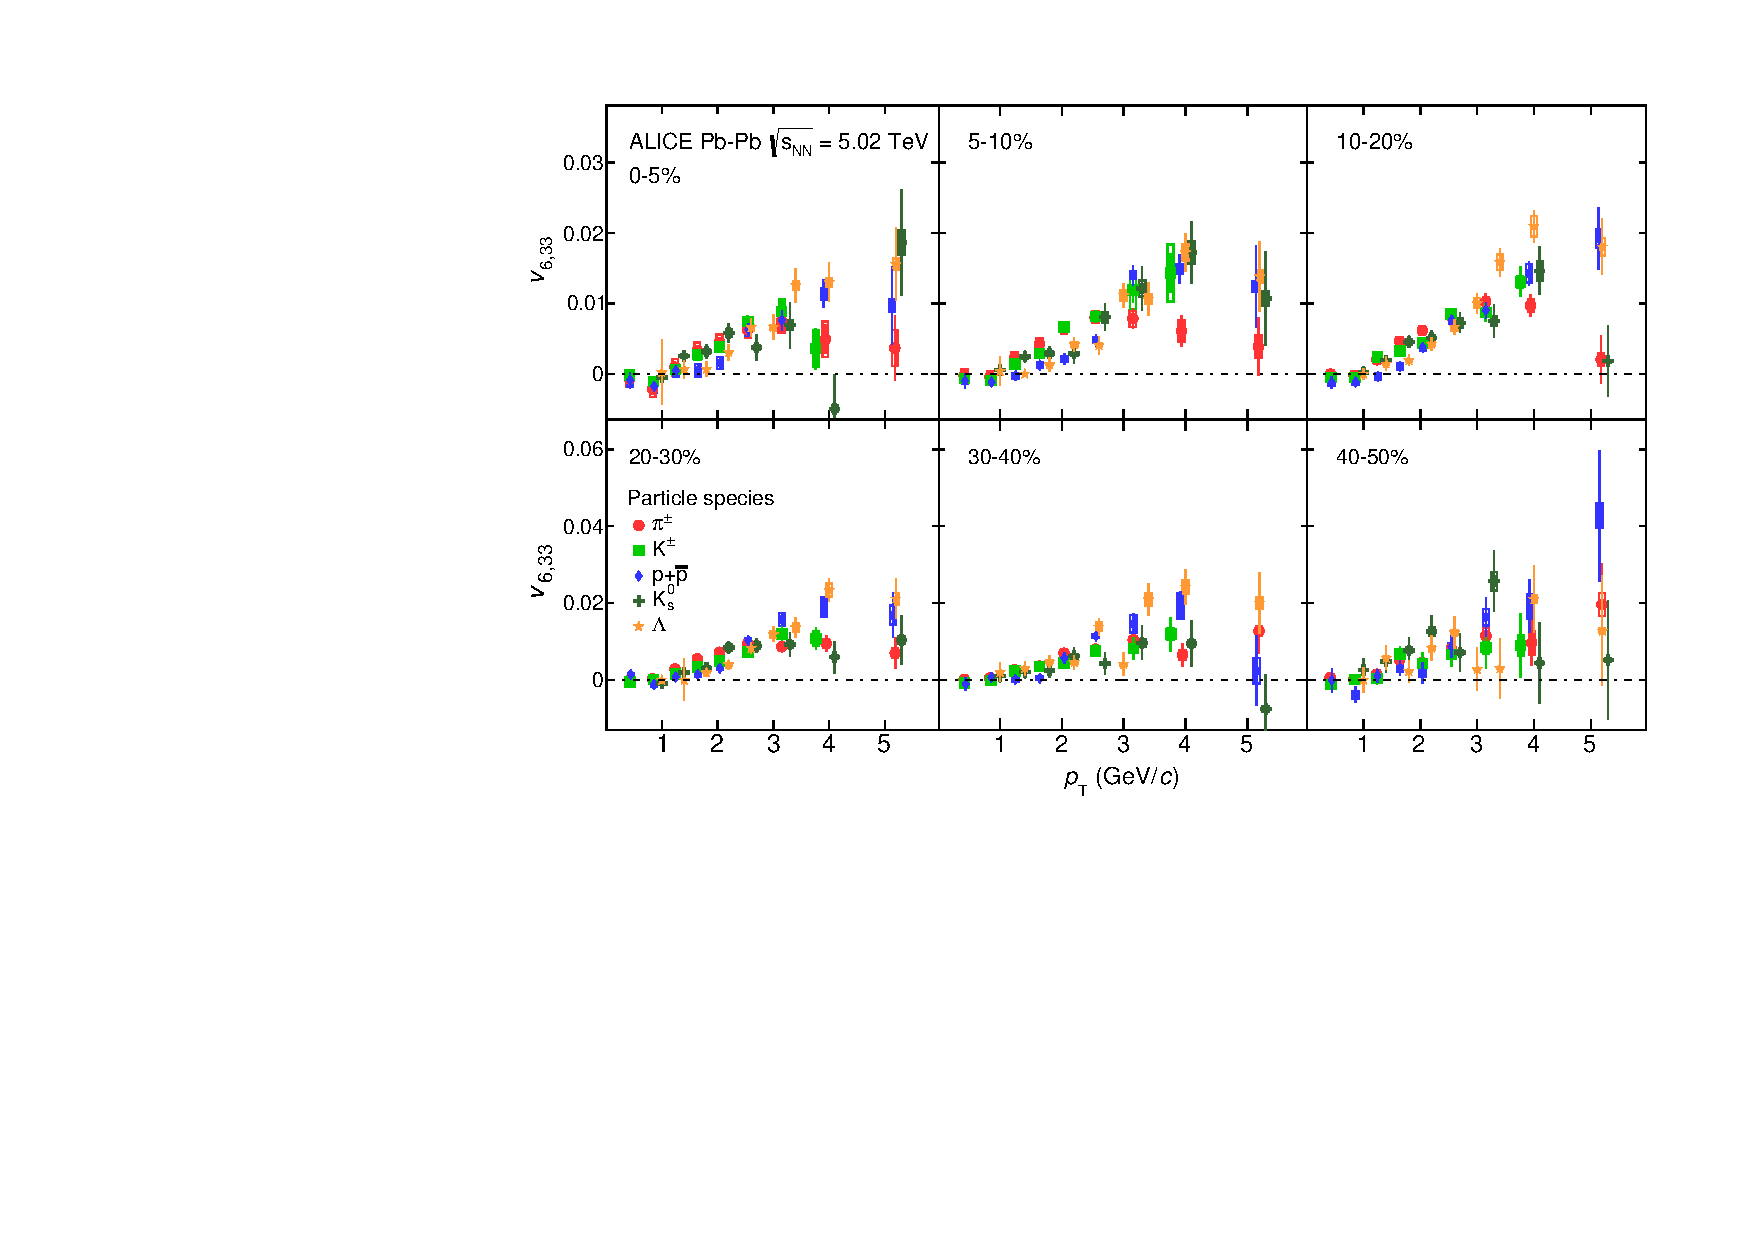
\includegraphics[scale=0.82]{figures/results/All_v633_gap00_PID2_3by2.pdf}

\end{center}
\caption{The \pT-differential $v_{6,33}$ for different particle species grouped into different centrality intervals of Pb--Pb collisions \sNN}
\label{v633_particleDependence}
\end{figure}

\begin{figure}[!htb]
\begin{center}
%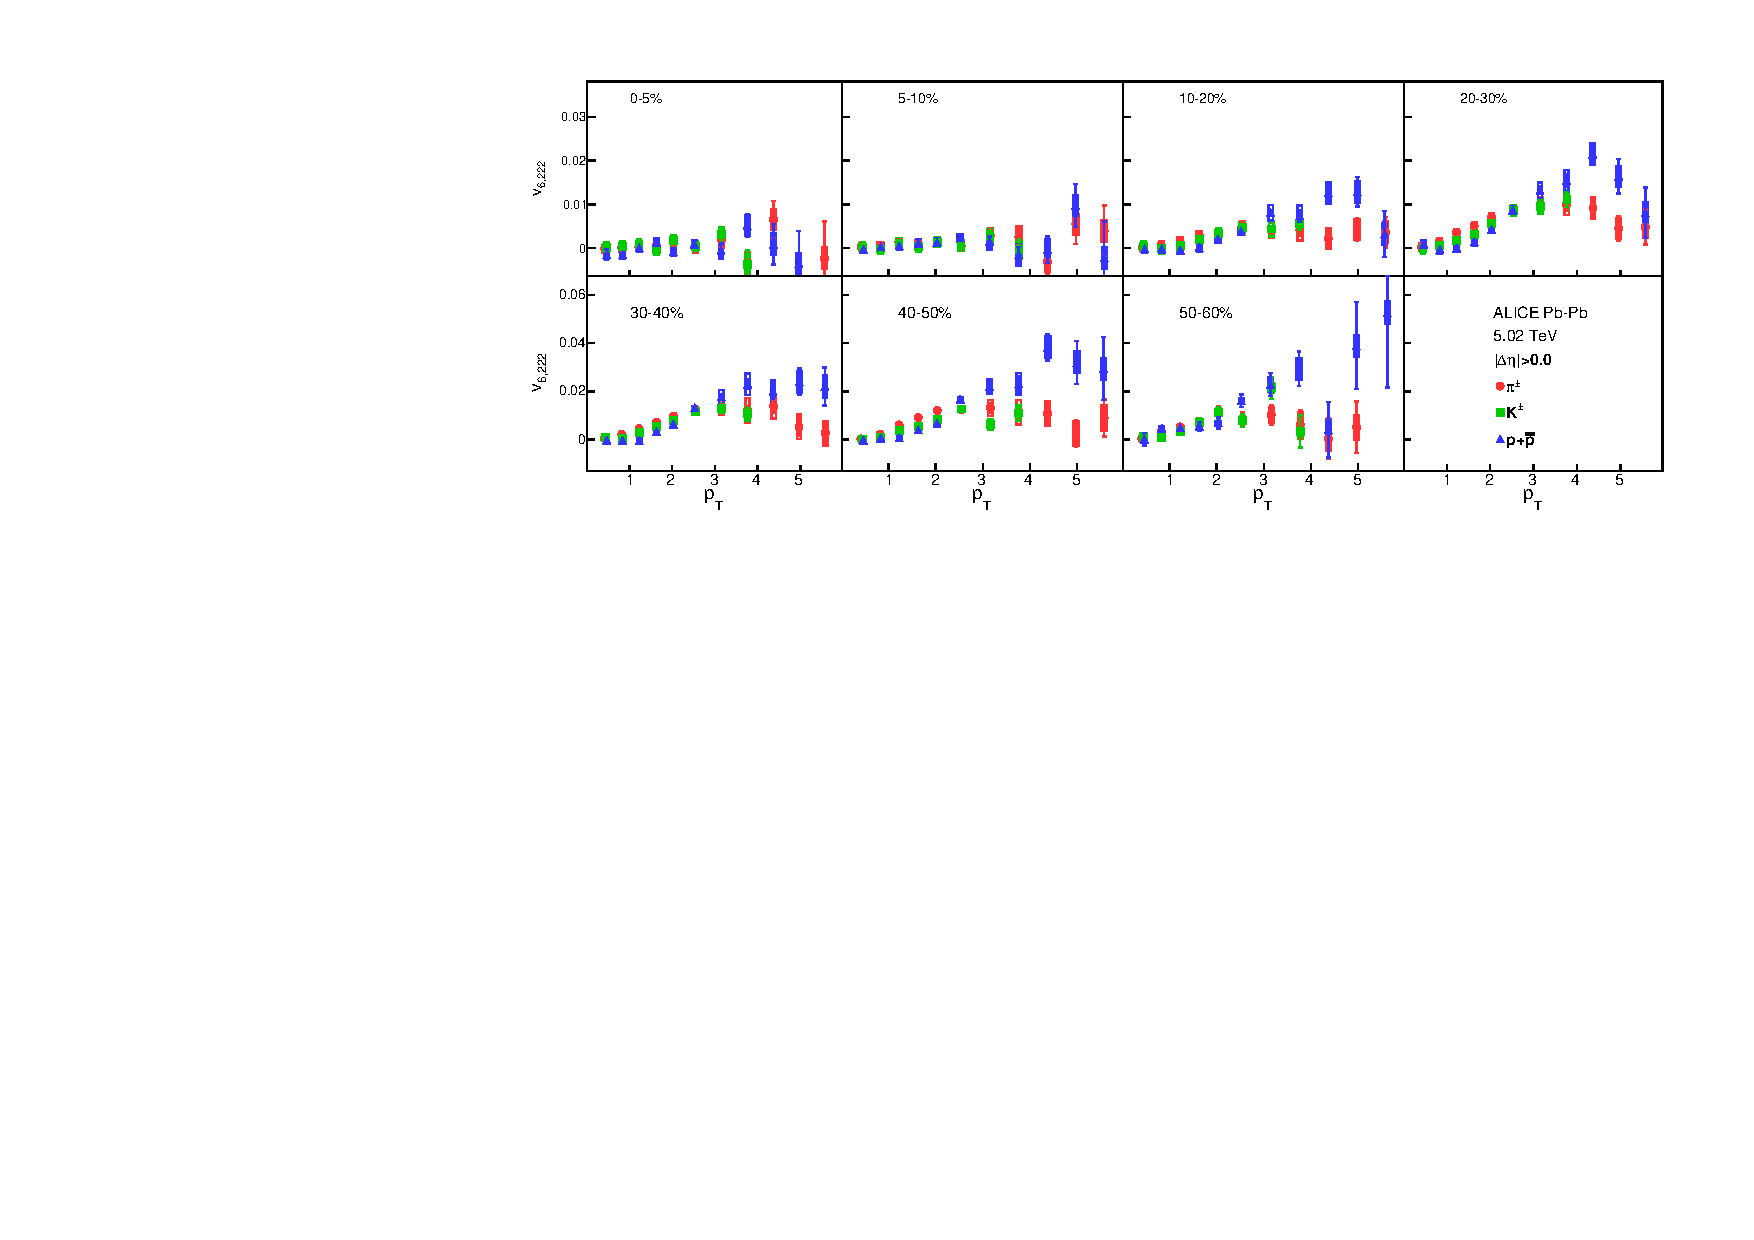
\includegraphics[scale=0.82]{figures/results/All_v6222_gap00.pdf}
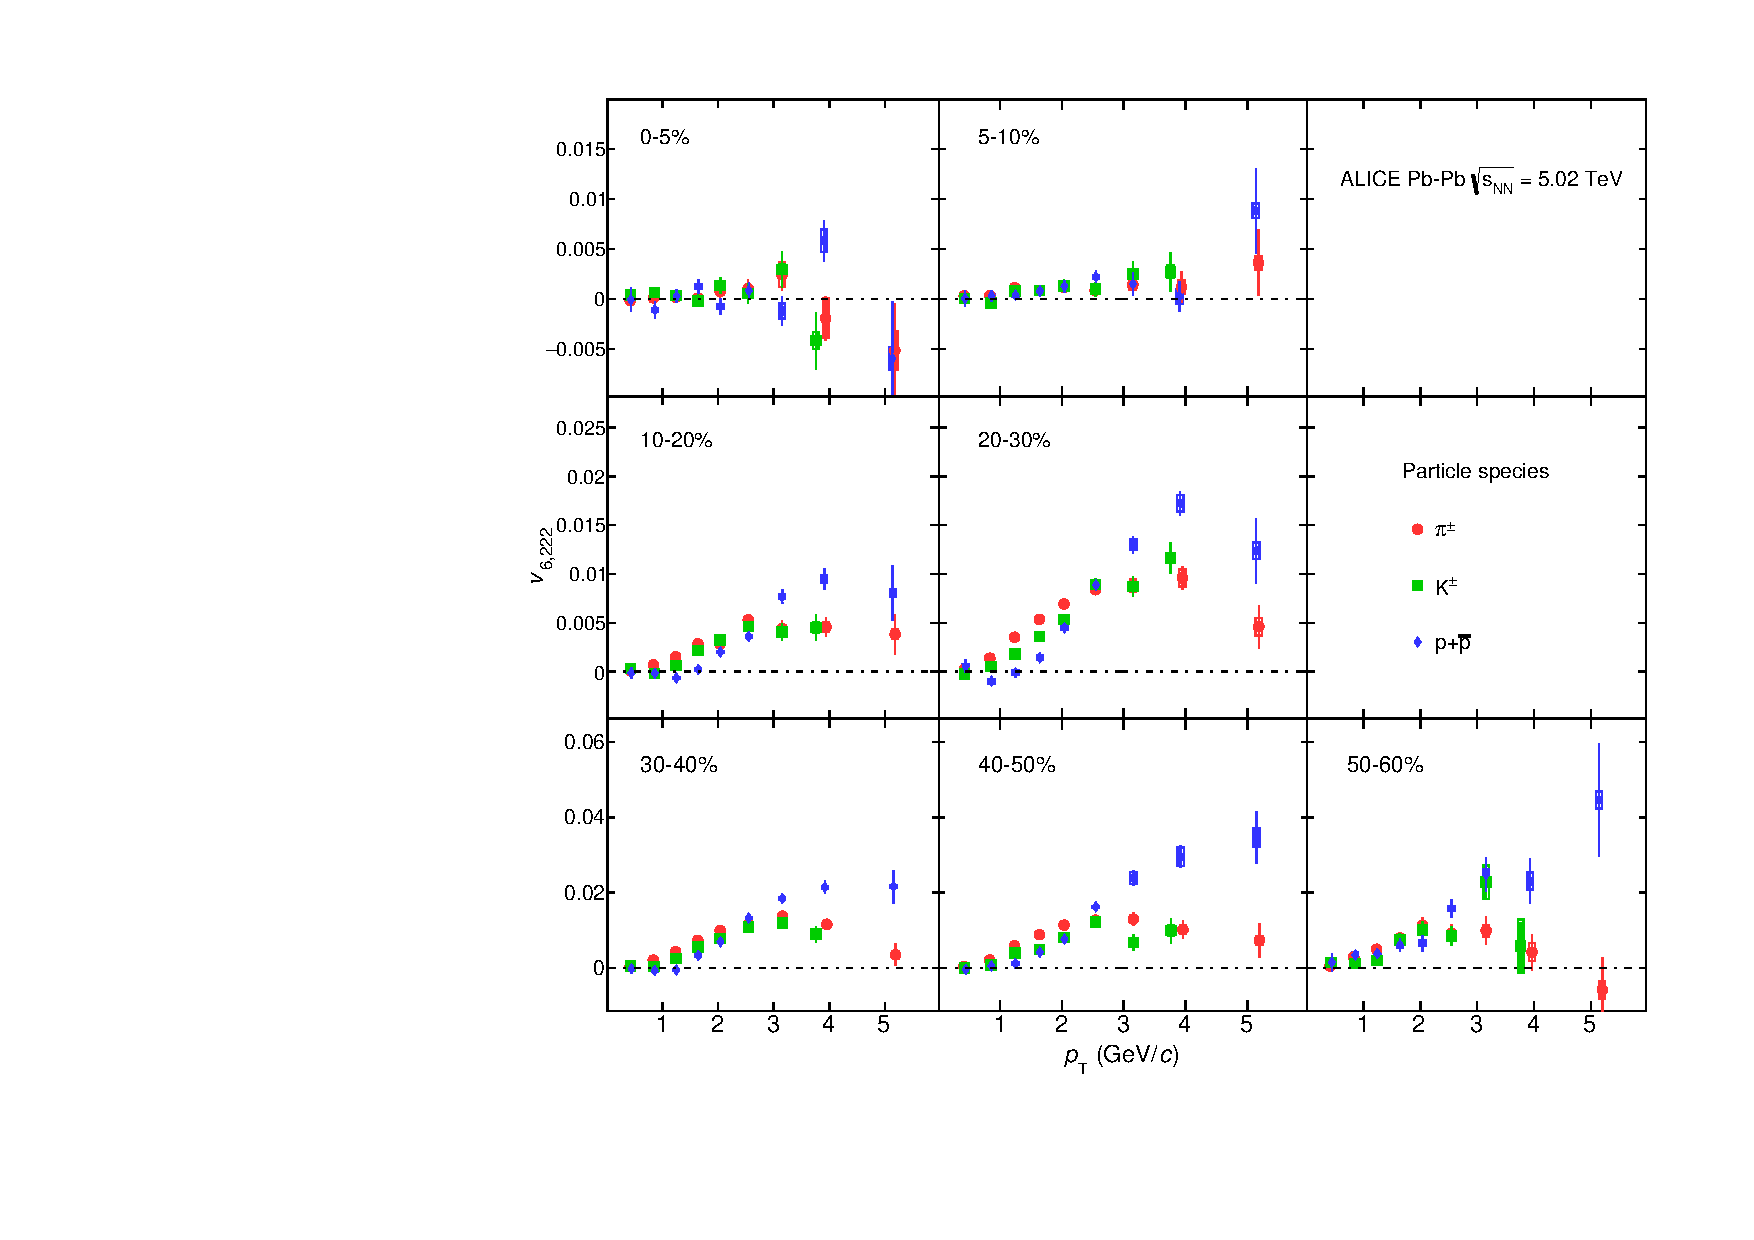
\includegraphics[scale=0.82]{figures/results/All_v6222_gap00_PID2_3by3.pdf}

\end{center}
\caption{The \pT-differential $v_{6,222}$ for different particle species grouped into different centrality intervals of Pb--Pb collisions \sNN}
\label{v6222_particleDependence}
\end{figure}

\newpage

In addition, in the intermediate \pT~region (for \pT $> 2.5$ \GeV) the data points of Figs. \ref{v422_particleDependence}-\ref{v6222_particleDependence} exhibit a particle type grouping. In particular, mesons (\pion, \kaon, \Ks~and $\phi$) and baryons (\proton~and \lambdas) group based on their type with $v_{n,mk}$ of baryons having a larger magnitude. This particle type grouping was previously seen in the anisotropic flow measurements \cite{Abelev:2014pua,Adam:2016nfo,Acharya:2018zuq,Adams:2003am,Abelev:2007qg,Adler:2003kt,Adare:2006ti} of various particle species triggering the development of calculations relying on coalescence. This suggests that flow develops at the parsonic stage and if so, combining two or three quarks to form hadronic states might result into hadrons inheriting the transverse momentum and subsequently, $v_{n}$ of their constituents. As a next step it was suggested to use a form of number of constituent quark (NCQ) scaling in which both flow coefficients and \pT~were scaled by the number of constituent quarks ($n_{q}$). This scaling, worked initially at RHIC energies, although later measurements revealed sizeable deviations from a perfect scaling \cite{Adams:2003am,Abelev:2007qg,Adler:2003kt,Adare:2006ti}. Recently, ALICE measurements showed that the NCQ scaling at LHC energies holds at best at an approximate level of 20\% for $v_{n}$ \cite{Abelev:2014pua,Adam:2016nfo,Acharya:2018zuq}. Various theoretical ideas were created to address the origin of possible scaling by requiring quark coalescence to be the dominant particle production mechanism in the intermediate \pT~region, where the hydrodynamic evolution of the fireball is not the driving force behind the development of anisotropic flow \cite{Voloshin:2002wa,Molnar:2003ff}.

%\subsection{Test of scaling properties}
%\label{subsection:NCQscaling}

Figures \ref{v422_NCQ}, \ref{v523_NCQ}, \ref{v633_NCQ} and \ref{v6222_NCQ} present $v_{4,22}$, $v_{5,32}$, $v_{6,33}$ and $v_{6,222}$ respectively, scaled by the inverse of number of constituent quarks ($n_{q}$) as a function of \pTnq~for \pion, \kaon, \proton, \Ks, \lambdas~and $\phi$-meson grouped in different centrality intervals. The scaling is consistent with the observations reported for higher order total flow coefficients \cite{Acharya:2018zuq}. Similarly, for non-linear modes this scaling hold at best at an approximate level ($\pm$20\%). 

\begin{figure}[!htb]
\begin{center}
%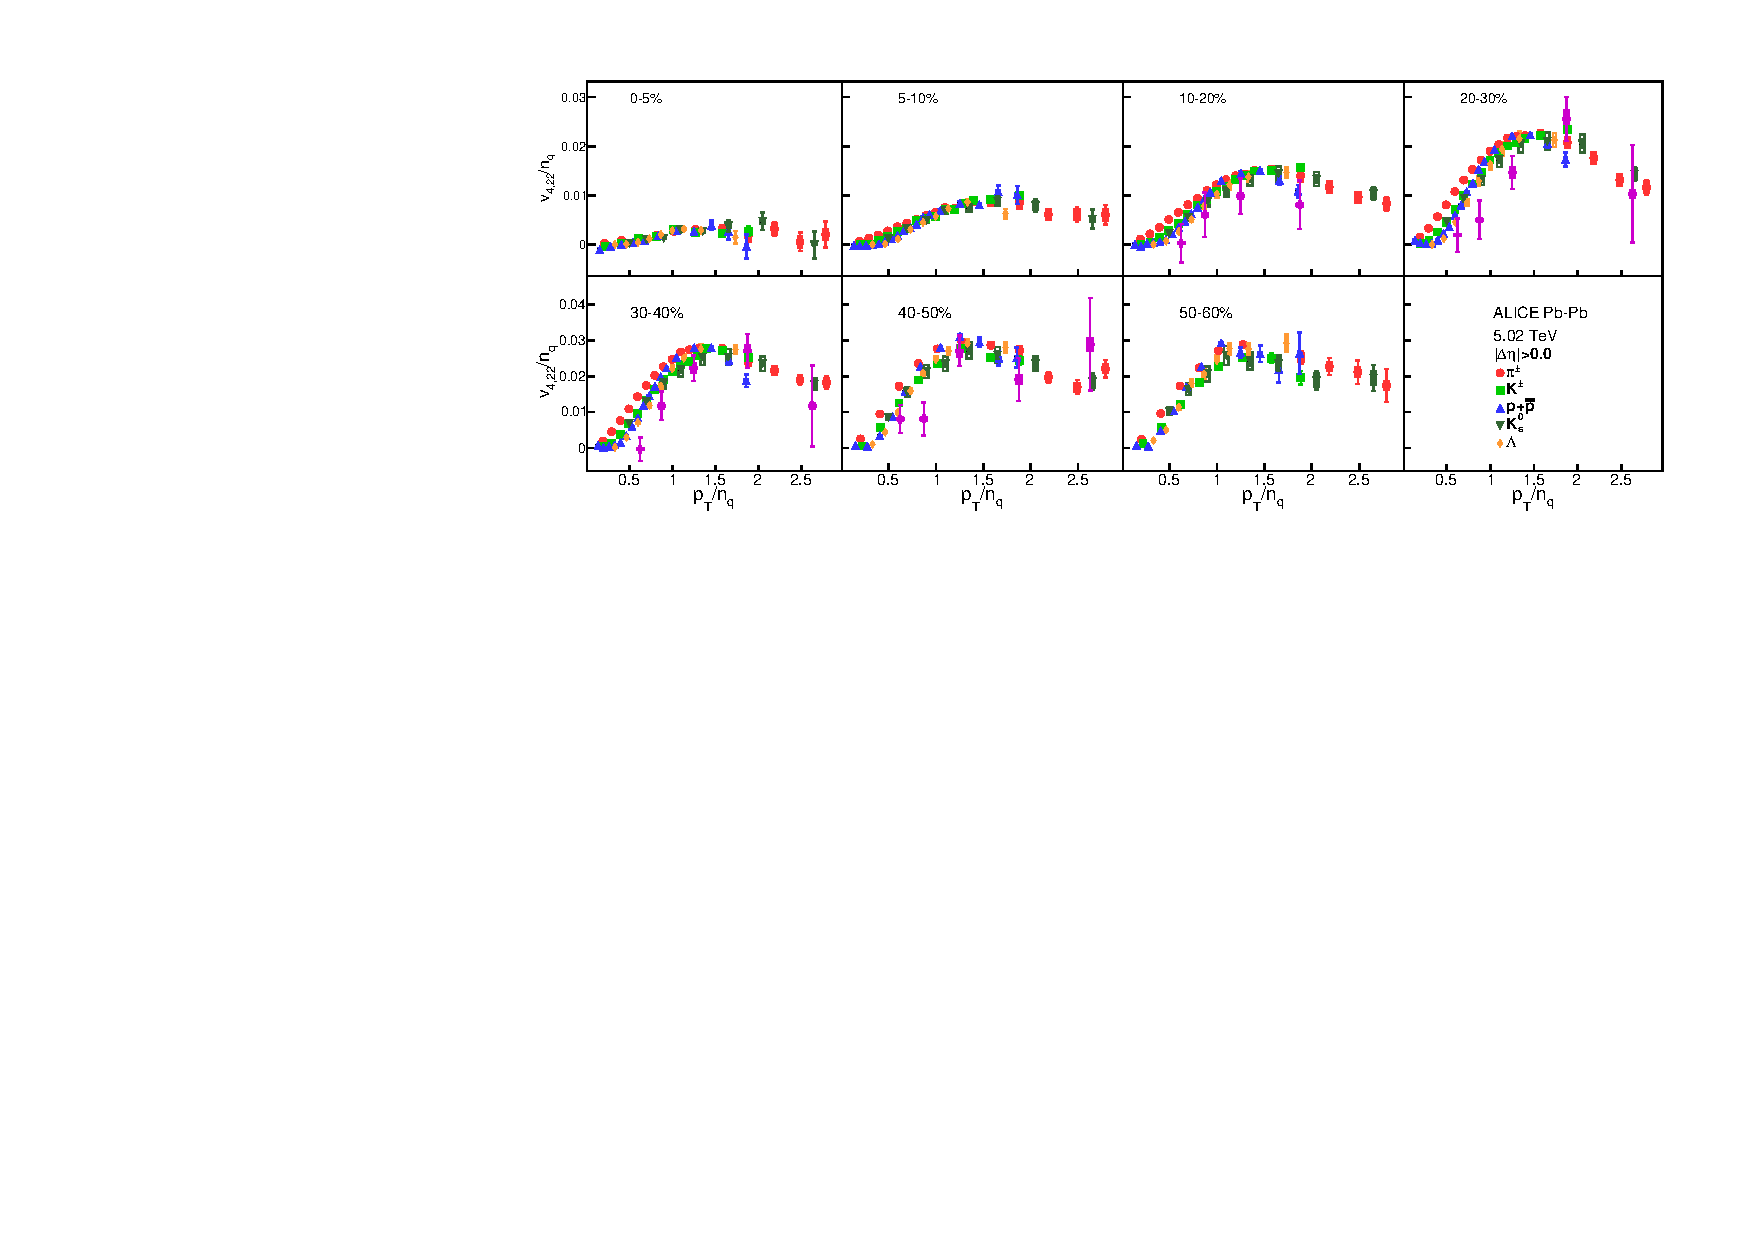
\includegraphics[scale=0.82]{figures/scaling/All_v422_gap00_NCQ.pdf}
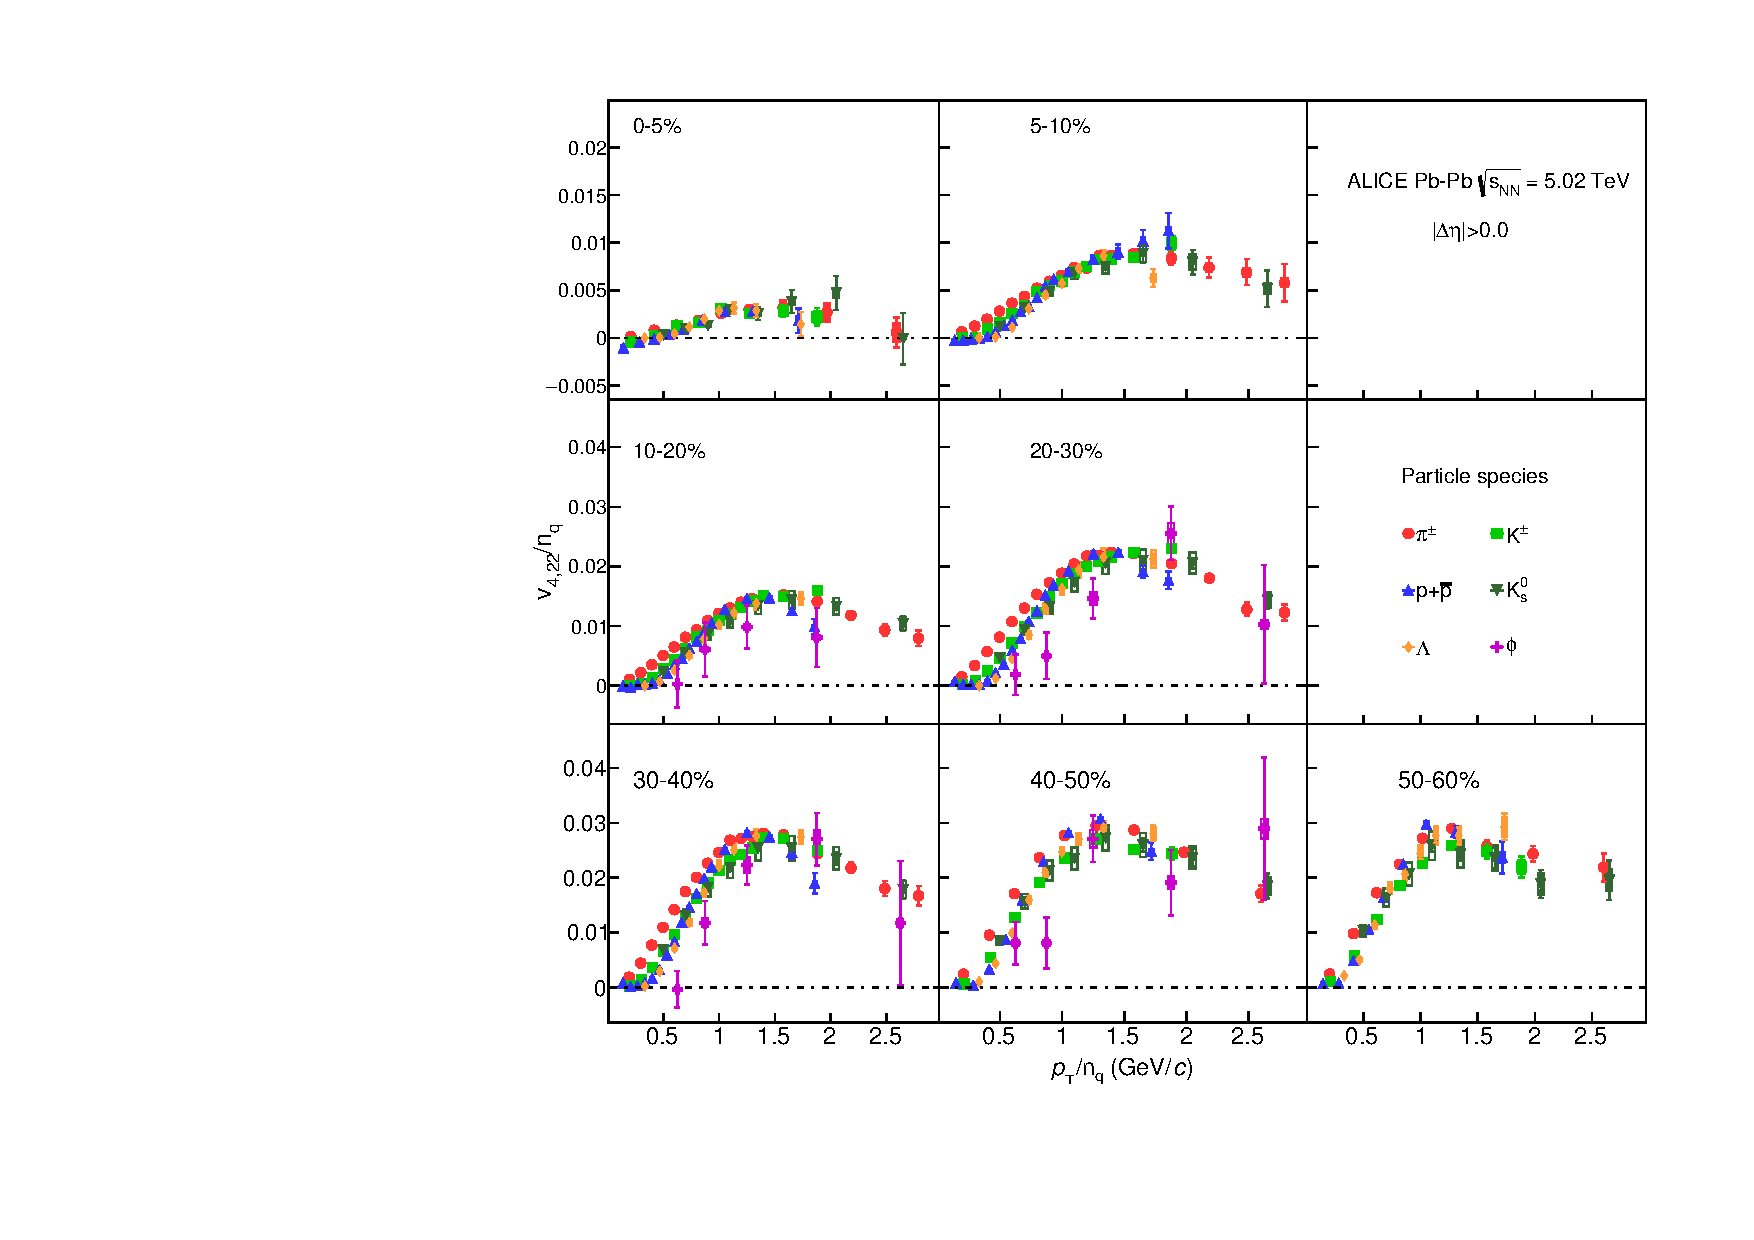
\includegraphics[scale=0.82]{figures/scaling/All_v422_gap00_NCQ_3by3.pdf}
\end{center}
\caption{The $p_{\rm{T}}/n_{q}$-dependence of $v_{4,22}/n_{q}$ for different particle species grouped into different centrality intervals of Pb--Pb collisions \sNN}
\label{v422_NCQ}
\end{figure}

\begin{figure}[!htb]
\begin{center}
%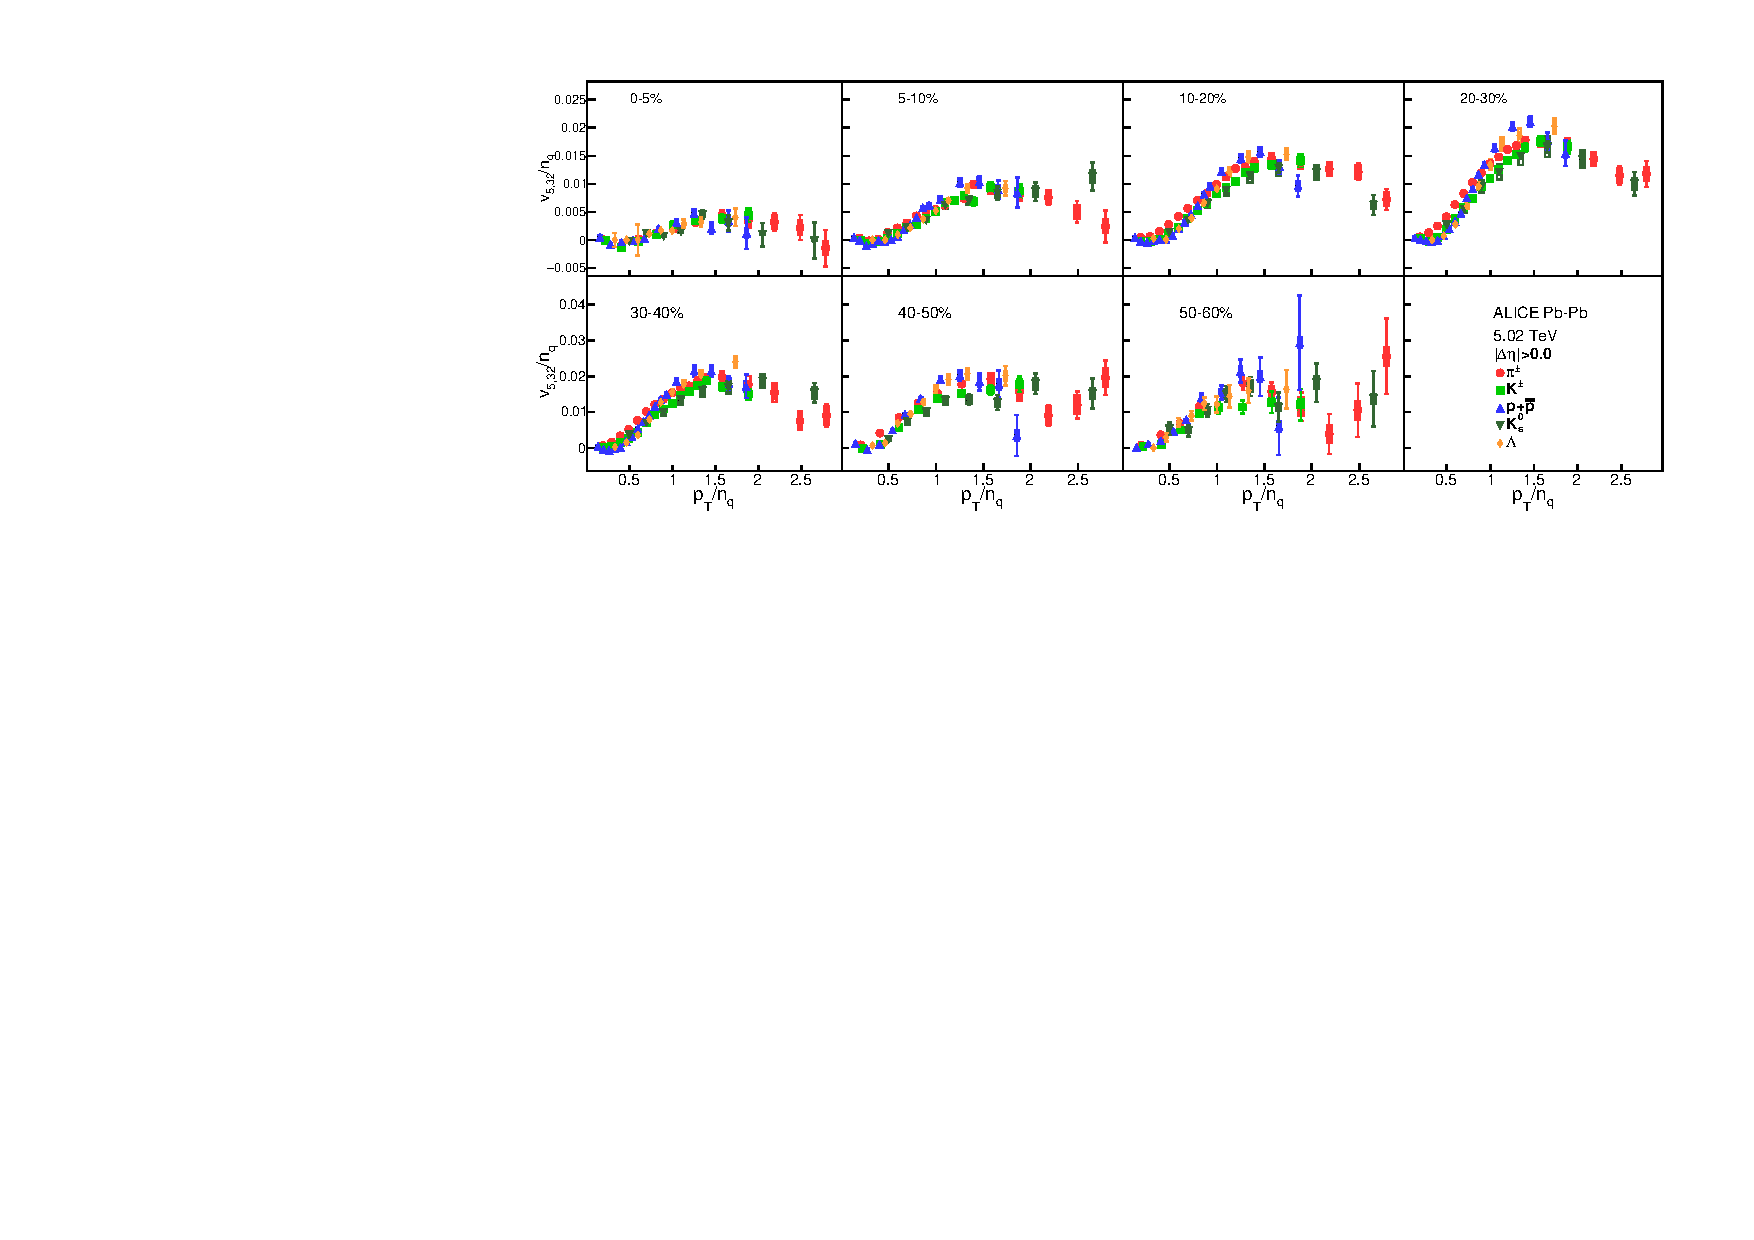
\includegraphics[scale=0.82]{figures/scaling/All_v523_gap00_NCQ.pdf}
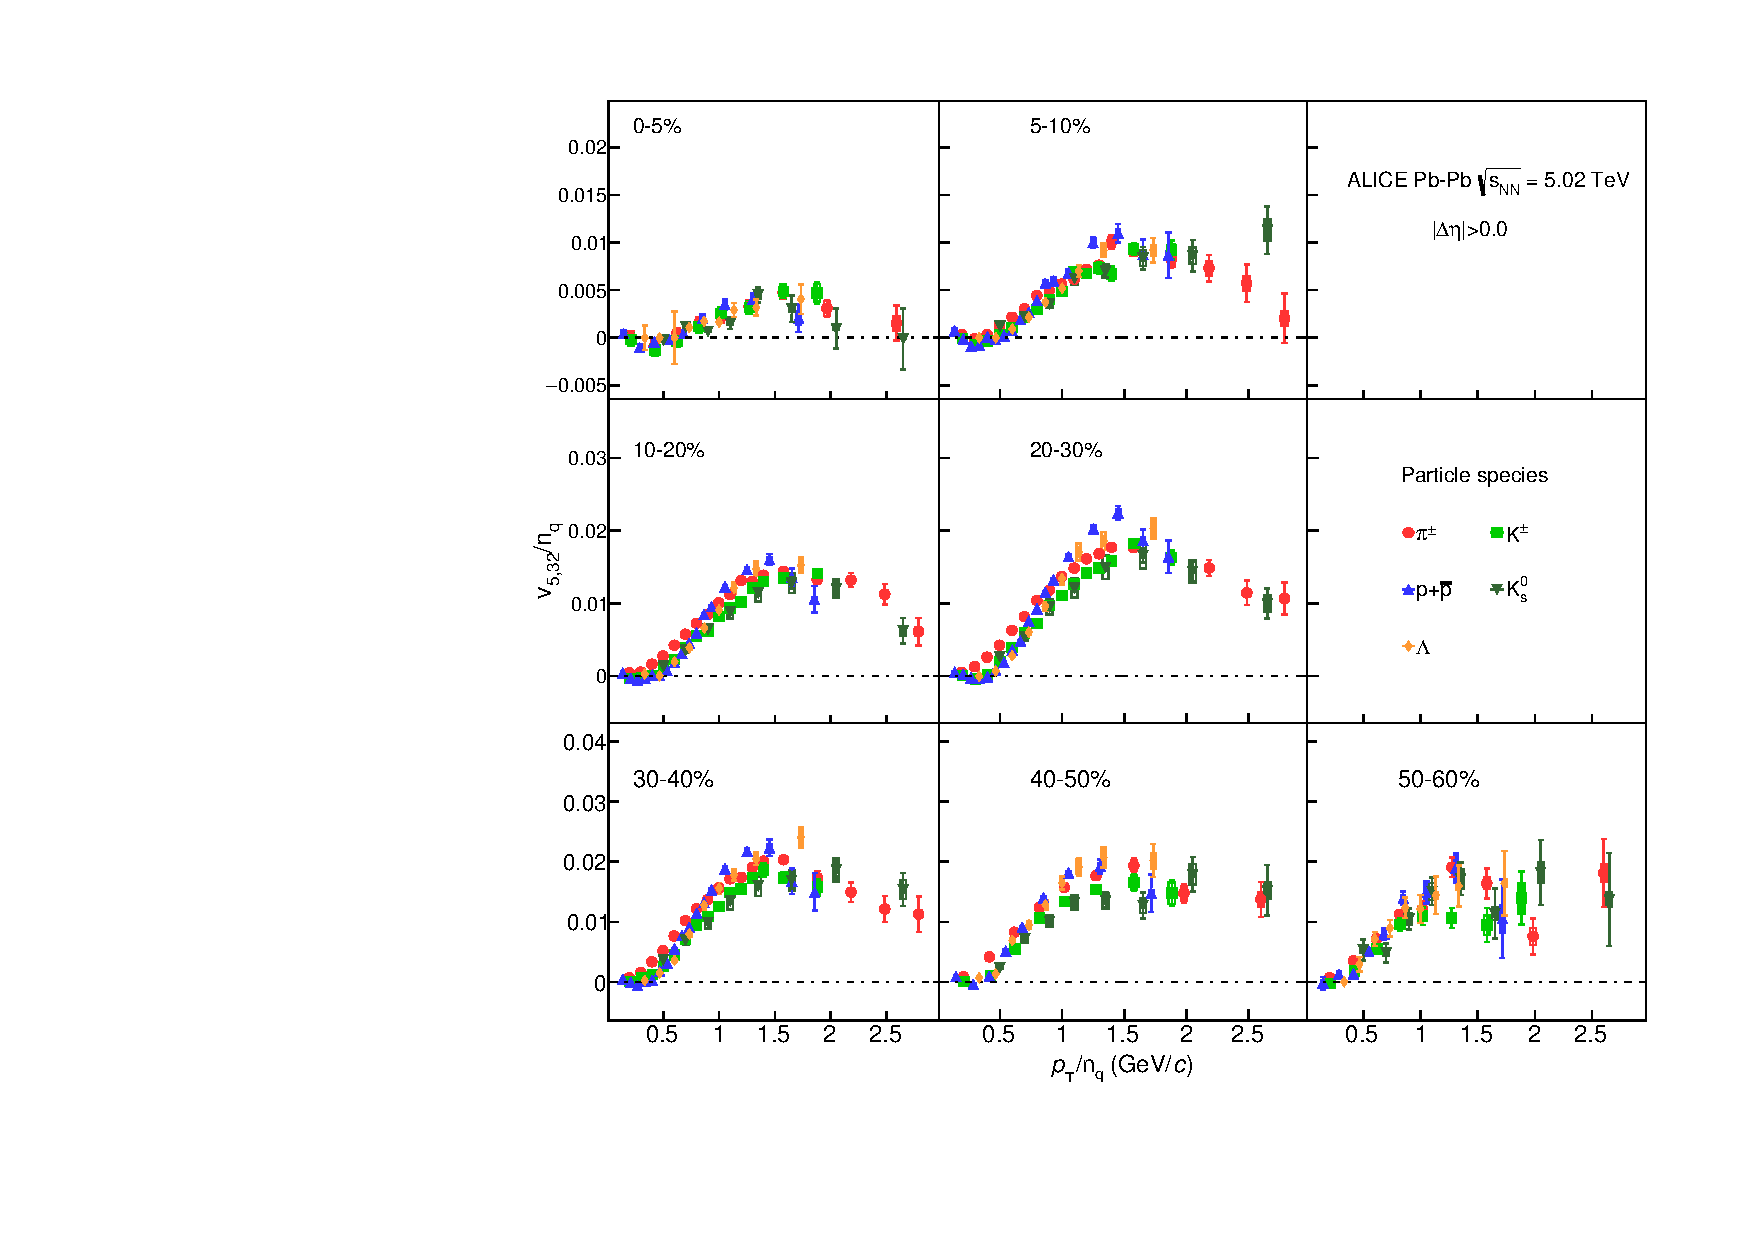
\includegraphics[scale=0.82]{figures/scaling/All_v523_gap00_NCQ_3by3.pdf}

\end{center}
\caption{The $p_{\rm{T}}/n_{q}$-dependence of $v_{5,32}/n_{q}$ for different particle species grouped into different centrality intervals of Pb--Pb collisions \sNN}
\label{v523_NCQ}
\end{figure}

\begin{figure}[!htb]
\begin{center}
%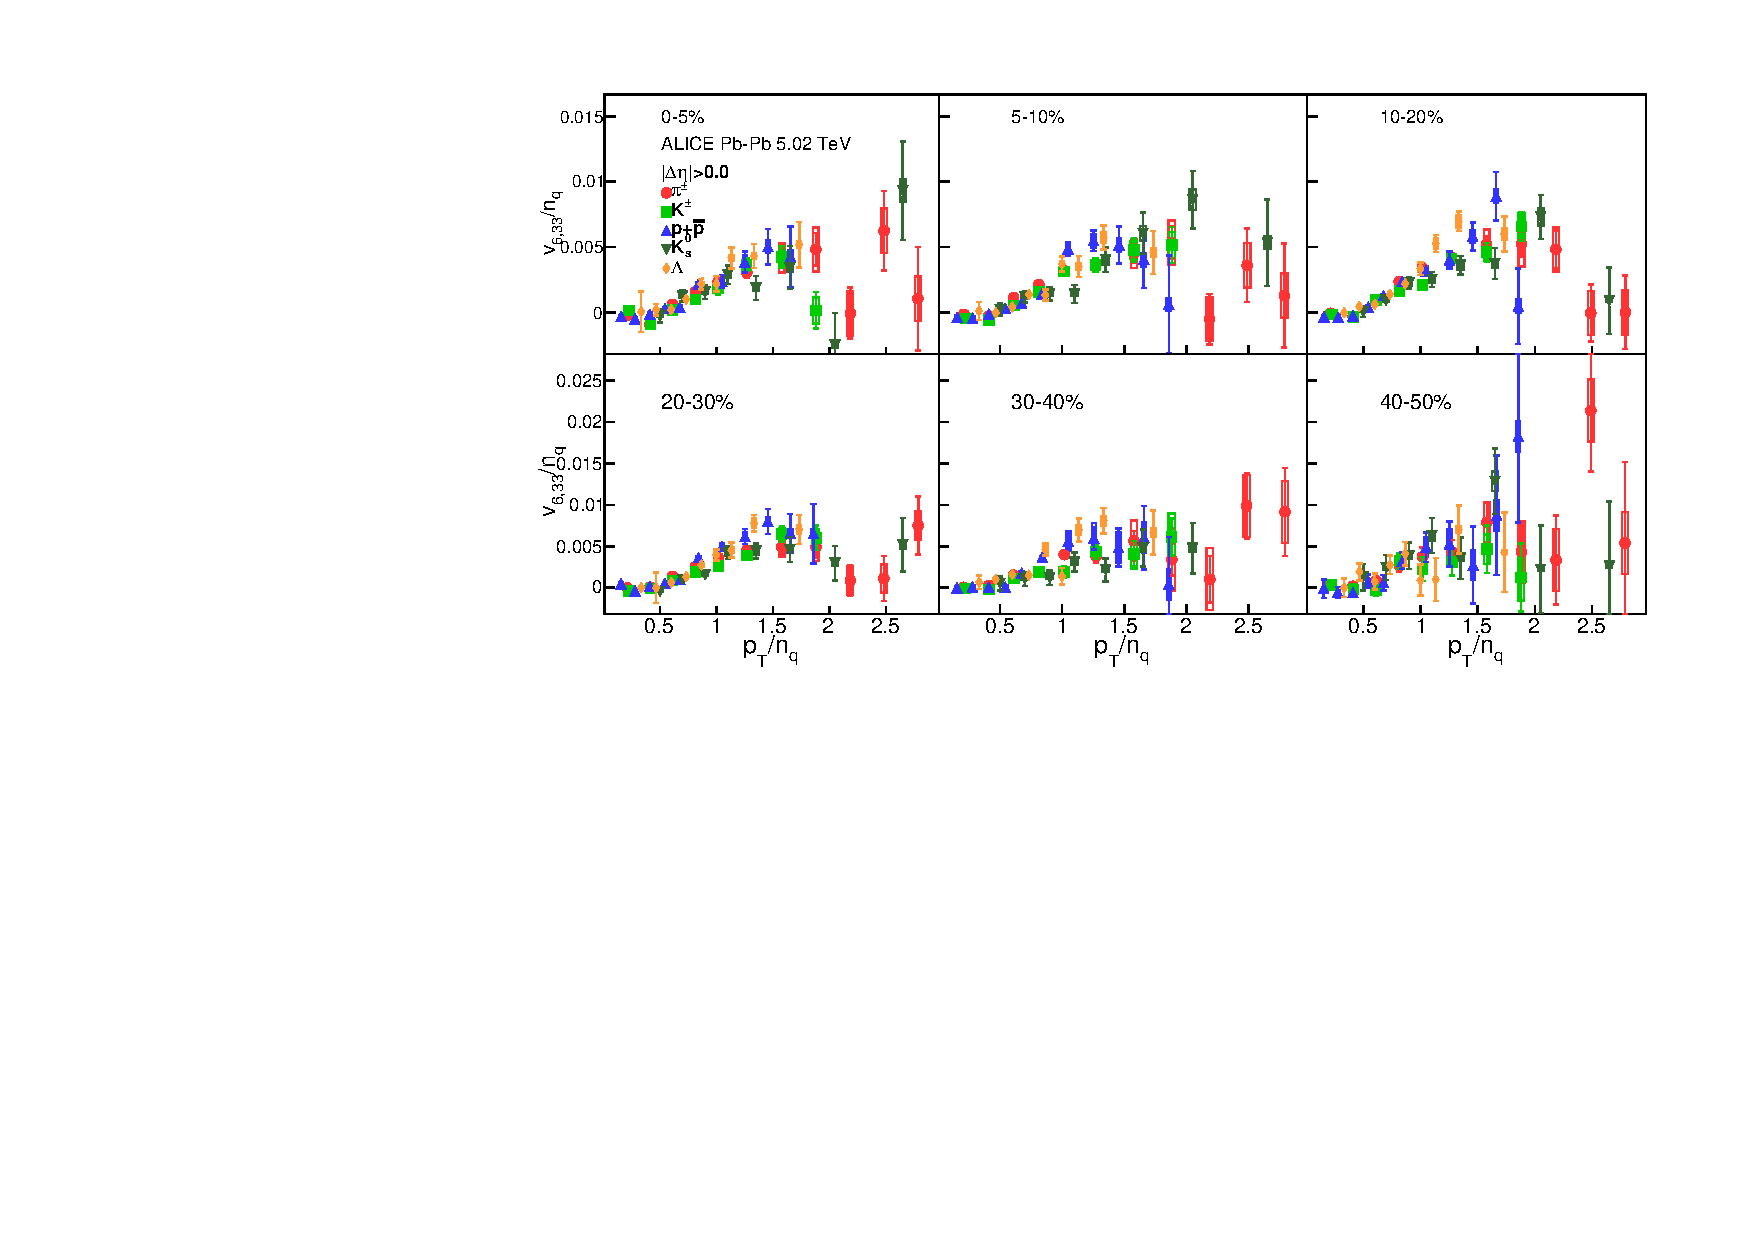
\includegraphics[scale=0.82]{figures/scaling/All_v633_gap00_NCQ.pdf}
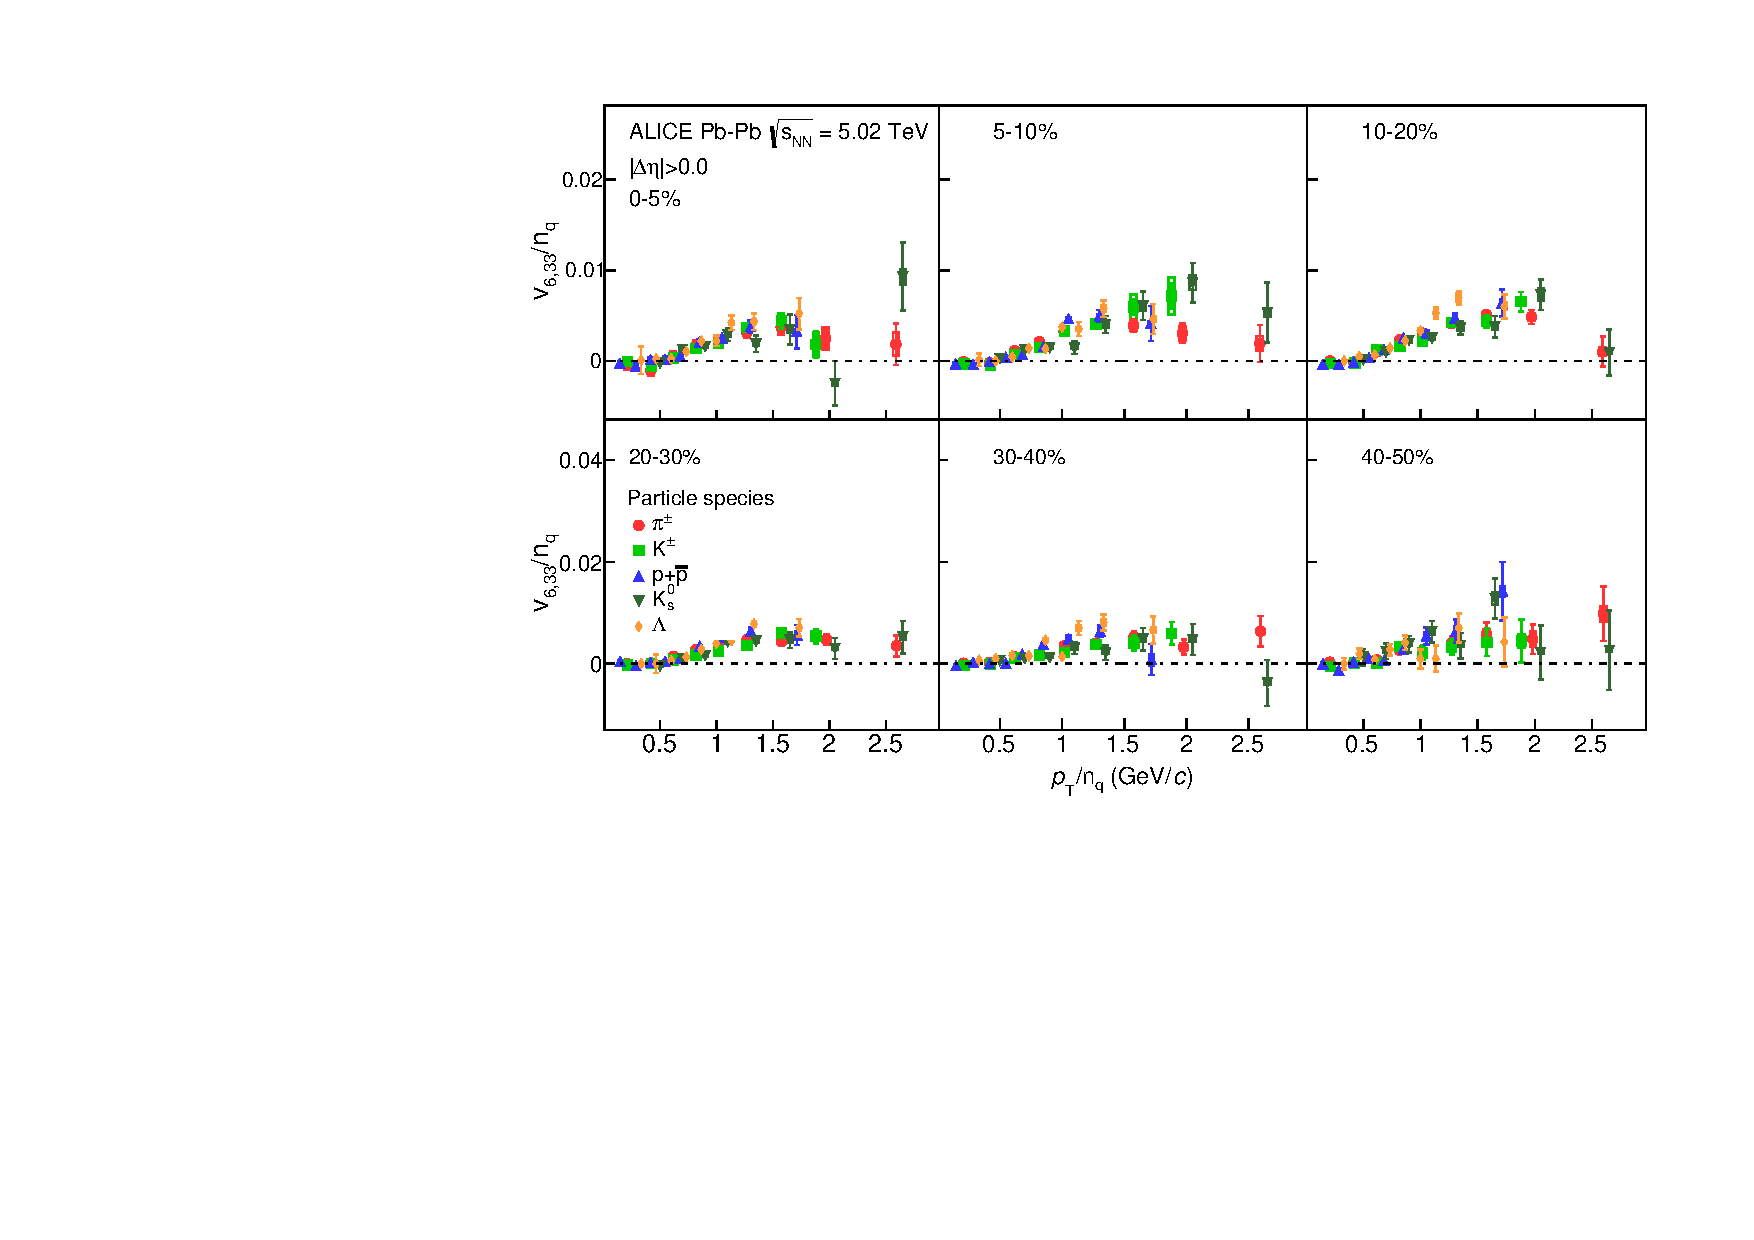
\includegraphics[scale=0.82]{figures/scaling/All_v633_gap00_NCQ_3by2.pdf}
\end{center}
\caption{The $p_{\rm{T}}/n_{q}$-dependence of $v_{6,33}/n_{q}$ for different particle species grouped into different centrality intervals of Pb--Pb collisions \sNN}
\label{v633_NCQ}
\end{figure}

\begin{figure}[!htb]
\begin{center}
%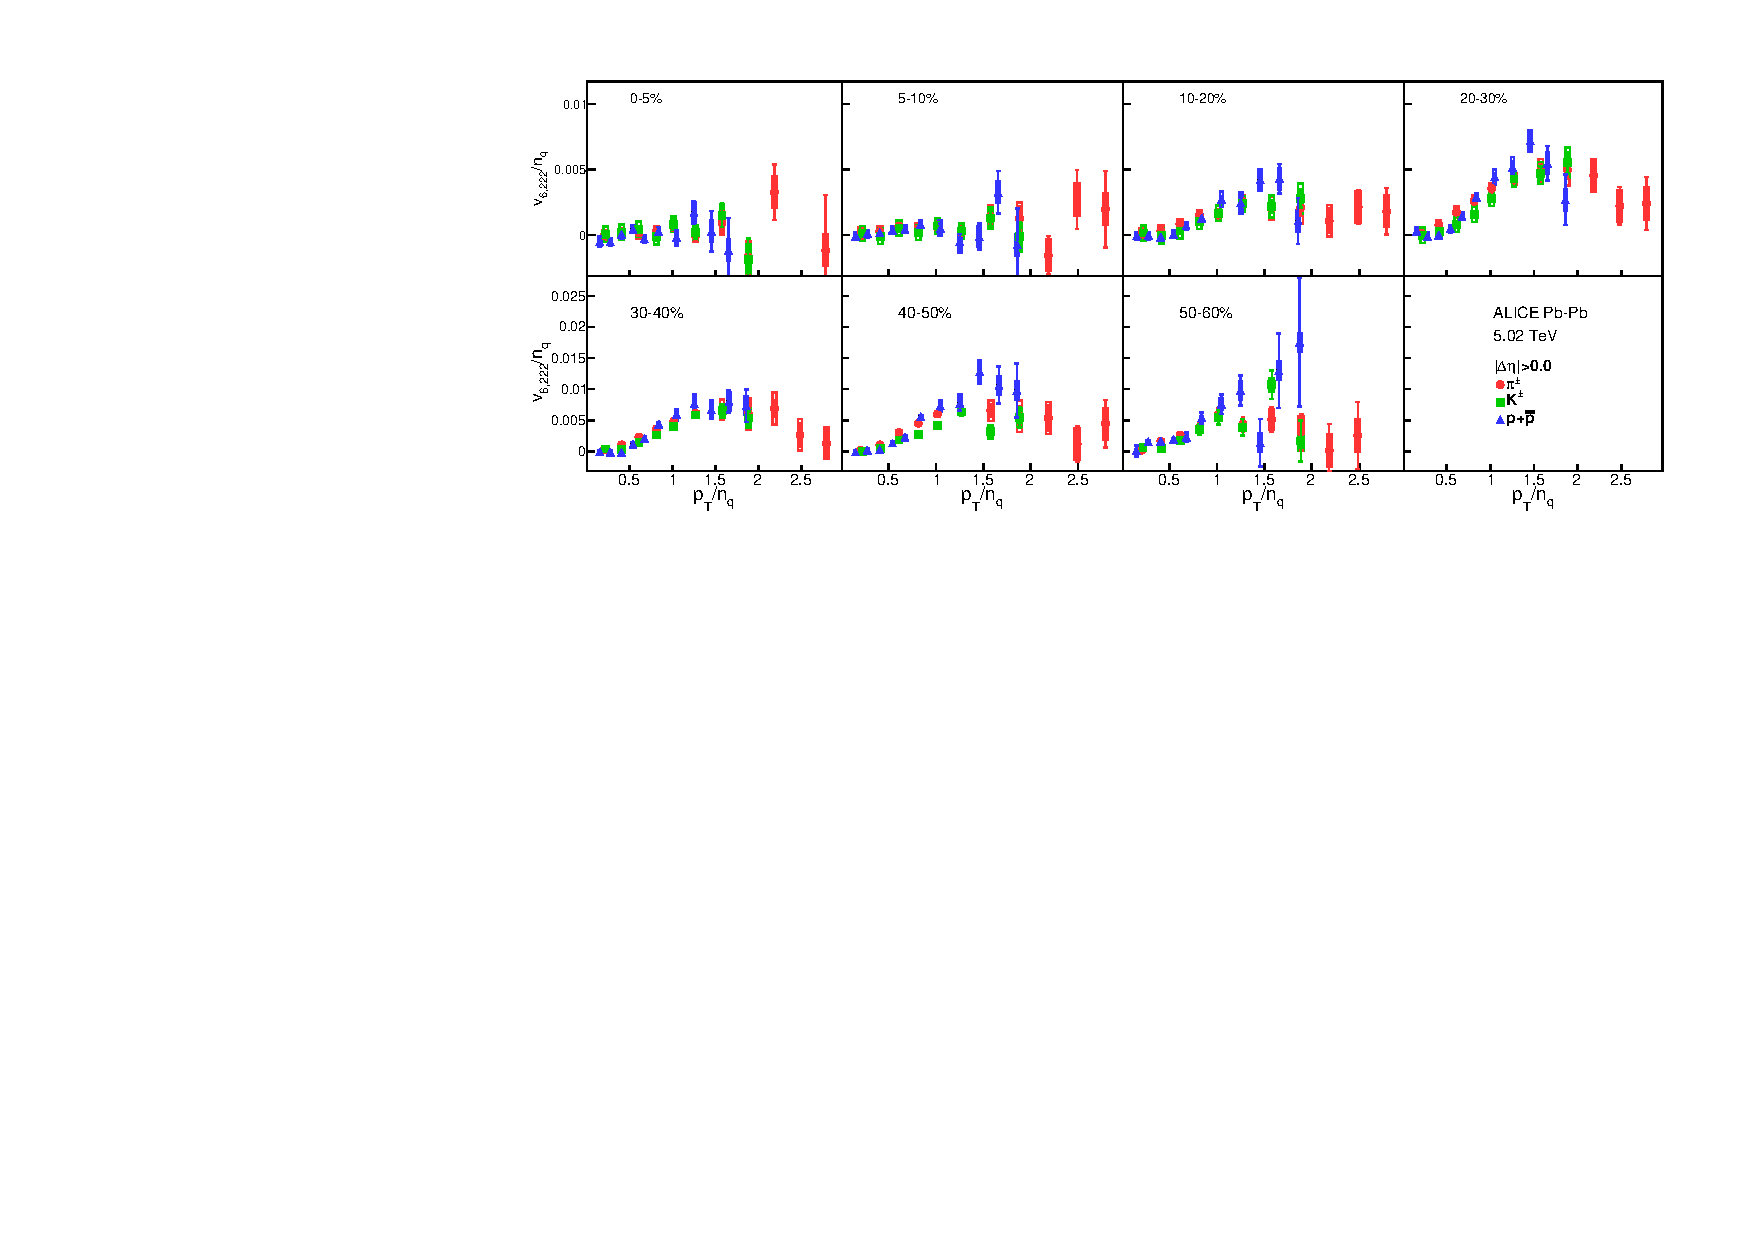
\includegraphics[scale=0.82]{figures/scaling/All_v6222_gap00_NCQ.pdf}
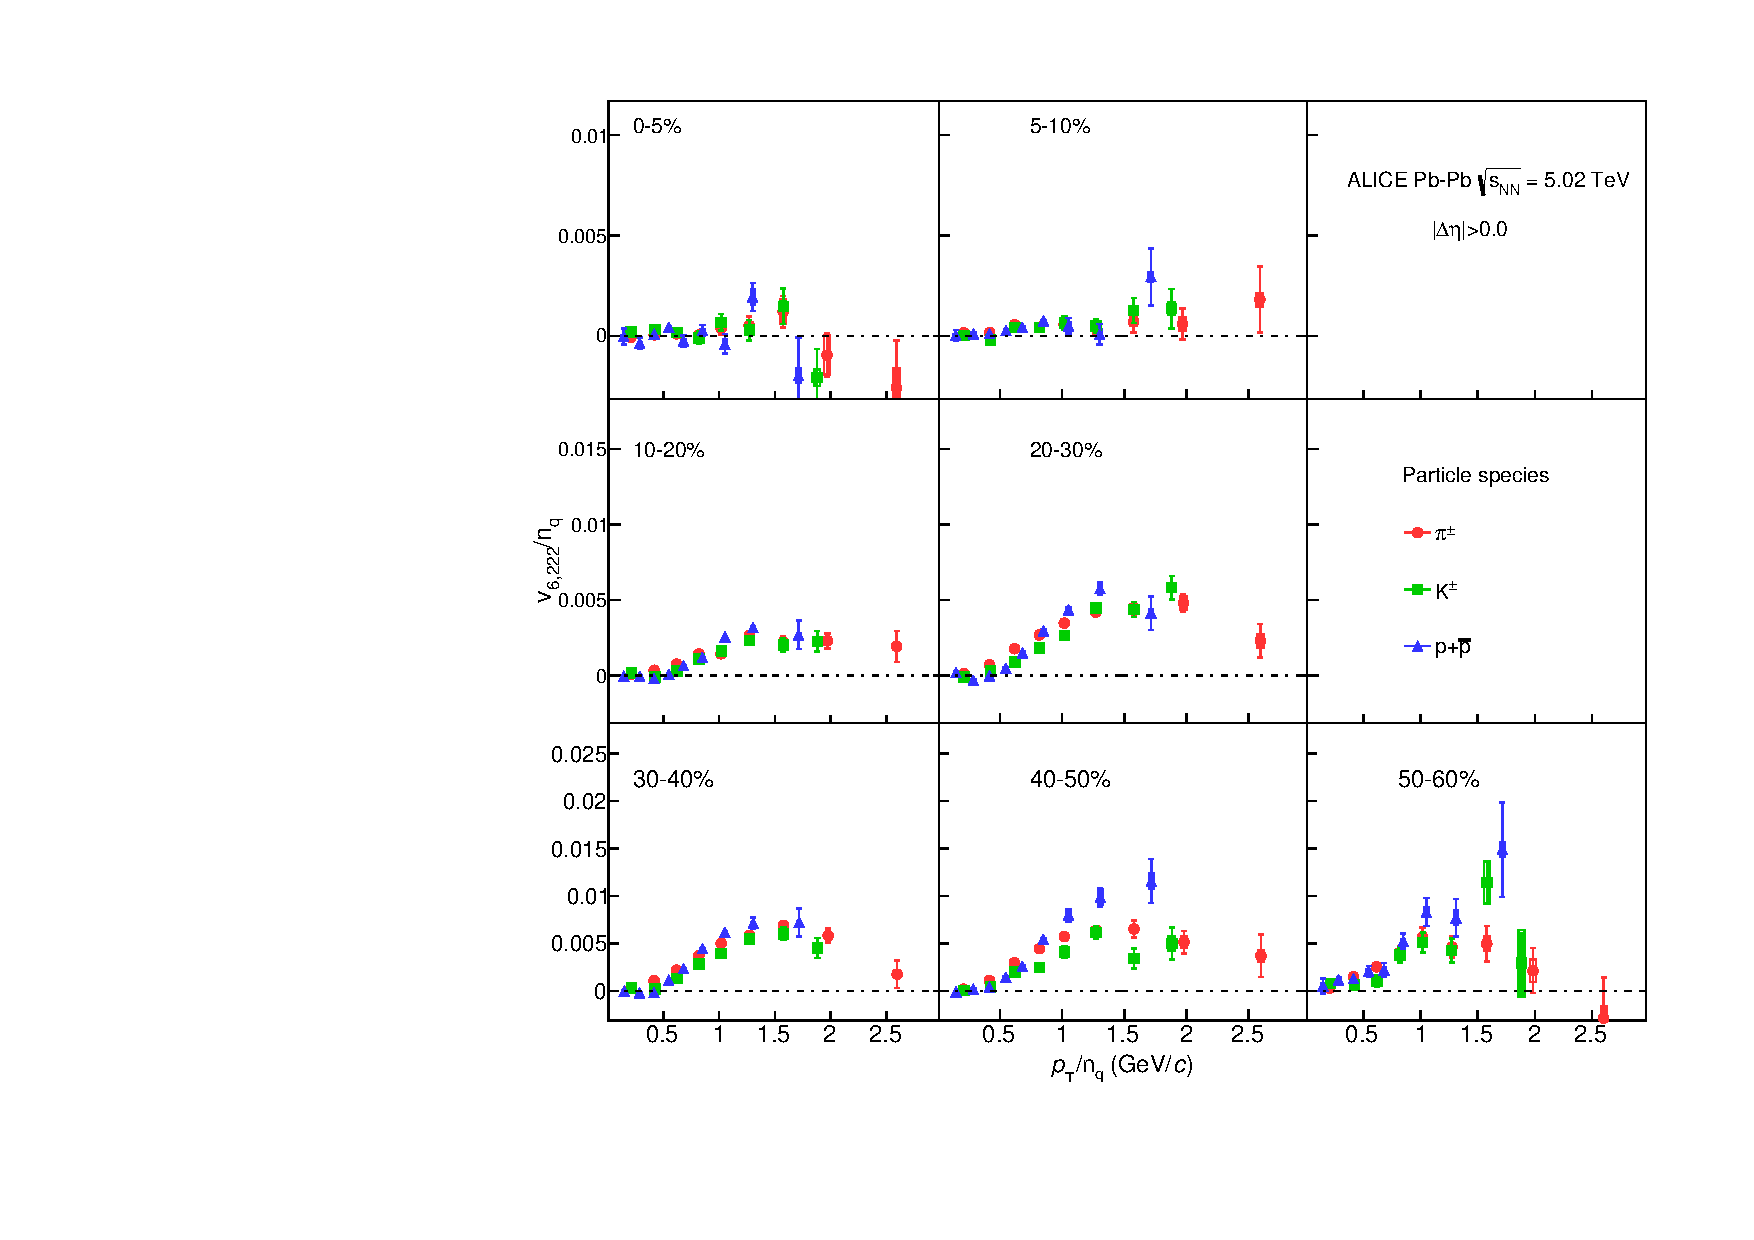
\includegraphics[scale=0.82]{figures/scaling/All_v6222_gap00_NCQ_3by3.pdf}

\end{center}
\caption{The $p_{\rm{T}}/n_{q}$-dependence of $v_{6,222}/n_{q}$ for different particle species grouped into different centrality intervals of Pb--Pb collisions \sNN}
\label{v6222_NCQ}
\end{figure}

\newpage
\subsection{Comparison with models}
\label{SubSec:hydro}

Measurements of total flow coefficients at RHIC and LHC are described well by hydrodynamic calculations \cite{Xu:2016hmp, McDonald:2016vlt, Zhao:2017yhj}. A recent comparison between total flow measurements at ALICE \cite{Acharya:2018zuq} and two hydrodynamic calculations from \cite{Zhao:2017yhj} shed new light on the initial conditions and the transport properties of the created system in Pb--Pb collisions. Both calculations are based on iEBE-VISHNU \cite{Shen:2014vra}, an event-by-event version of the VISHNU hybrid model \cite{Song:2010aq} coupling $2+1$~dimensional viscous hydrodynamics (VISH2+1) \cite{Song:2007fn} to a hadronic cascade model (UrQMD). The initial conditions used for these calculations are described by AMPT \cite{Lin:2004en} and TRENTo \cite{Moreland:2014oya} both with $\tau_{0}$=0.6 fm/$c$ and $T_{sw}$ =148 MeV \cite{Bernhard:2016tnd}. These values are obtained by using Bayesian statistics from a simultaneous fit of final charged-particle density, mean transverse momentum, and integrated total flow coefficients $v_{n}$ in Pb--Pb collisions at $\sqrt{s_{\rm NN}}$ = 2.76 TeV. For  AMPT initial conditions, constant values of specific shear viscosity ($\eta/s =0.08$, the lower limit conjectured by AdS/CFT) and bulk viscosity ($\zeta/s = 0$) are utilised, and TRENTo \cite{Moreland:2014oya} initial conditions incorporates a temperature dependent specific shear and bulk viscosity. \footnote{ For simplicity in the rest of this article the model with AMPT initial conditions, $\eta/s =0.08$ and $\zeta/s =0$ is referred to as AMPT and the model with TRENTo initial conditions, $\eta/s(\rm{T})$ and $\zeta/s(\rm{T})$ is referred to as TRENTo.} The comparison between the total flow measurements and these two calculations illustrates a qualitative agreement. This agreement between the data and the models depends on the particle species, transverse momentum range and centrality percentile and overall the AMPT model reproduces these measurements more accurately than TRENTo \cite{Acharya:2018zuq}.

Recently, it was shown that the \pT-integrated non-linear flow modes are good observables to constrain the initial conditions and transport properties of the system \cite{Acharya:2017zfg}. To further constrain the initial conditions and transport properties of the system and test the validity of these hydrodynamic models a comparison is performed between the measured \pT-dependent non-linear flow modes for \pion, \kaon~and \proton~with two hydrodynamical calculations from \cite{Zhao:2017yhj} as were used in comparison to the total flow measurements \cite{Acharya:2018zuq}. 


%To test the validity of these hydrodynamic models a comparison is performed between the measured non-linear flow modes and two hydrodynamical calculations from \cite{Zhao:2017yhj}.  Both calculations are based on iEBE-VISHNU \cite{Shen:2014vra}, an event-by-event version of the VISHNU hybrid model \cite{Song:2010aq} coupling $2+1$~dimensional viscous hydrodynamics (VISH2+1) \cite{Song:2007fn} to a hadronic cascade model (UrQMD). One of these models uses AMPT \cite{Lin:2004en} initial conditions with constant values of specific shear viscosity ($\eta/s =0.08$, the lower limit conjectured by AdS/CFT) and bulk viscosity ($\zeta/s = 0$), and the other model incorporates TRENTo \cite{Moreland:2014oya} initial conditions with a temperature dependent specific shear and bulk viscosity. 

%Both calculations are based on iEBE-VISHNU \cite{Shen:2014vra}, an event-by-event version of the VISHNU hybrid model \cite{Song:2010aq} coupling $2+1$~dimensional viscous hydrodynamics (VISH2+1) \cite{Song:2007fn} to a hadronic cascade model (UrQMD). One of these models uses AMPT \cite{Lin:2004en} initial conditions with constant values of specific shear viscosity ($\eta/s =0.08$, the lower limit conjectured by AdS/CFT) and bulk viscosity ($\zeta/s = 0$), and the other model incorporates TRENTo \cite{Moreland:2014oya} initial conditions with a temperature dependent specific shear and bulk viscosity. 

Figures \ref{v422_model}, \ref{v523_model}, \ref{v633_model} and \ref{v6222_model} present the comparison between the measurements (data points in the plots) and both models for the \pT-differential $v_{4,22}$, $v_{5,32}$, $v_{6,33}$ and $v_{6,222}$, respectively, for \pion, \kaon~and \proton~at 0-10\% up to 50-60\% centrality interval (40-50\% centrality interval for $v_{6,33}$) of Pb--Pb collisions at \sNN. The solid bands show the AMPT model and the hatched bands represent the TRENTo calculations. The bottom panels in each plot in Figs. \ref{v422_model}, \ref{v523_model}, \ref{v633_model} and \ref{v6222_model} present the difference between the models and the measurement. Both models produce a mass ordering in $p_{\rm{T}}<2.5$ \GeV. The comparison between the models and the the measurements of $v_{4,22}$ reveals that in more central collisions they reproduce the data however as centrality decreases the models start to deviate from the data. This pattern repeats for $v_{5,32}$ in which AMPT reproduces the data relatively better. The comparison between the measurements and the models  for $v_{6,222}$ and $v_{6,33}$ shows that the models are able to reproduce the data only up to 30-40\% and 20-30\% centrality intervals, respectively. 


%The comparisons show slightly better agreement between the data and the model which uses AMPT as the initial conditions but both models need to be tuned to data further to describe these sensitive flow modes.

 \begin{figure}[!htb]
\begin{center}
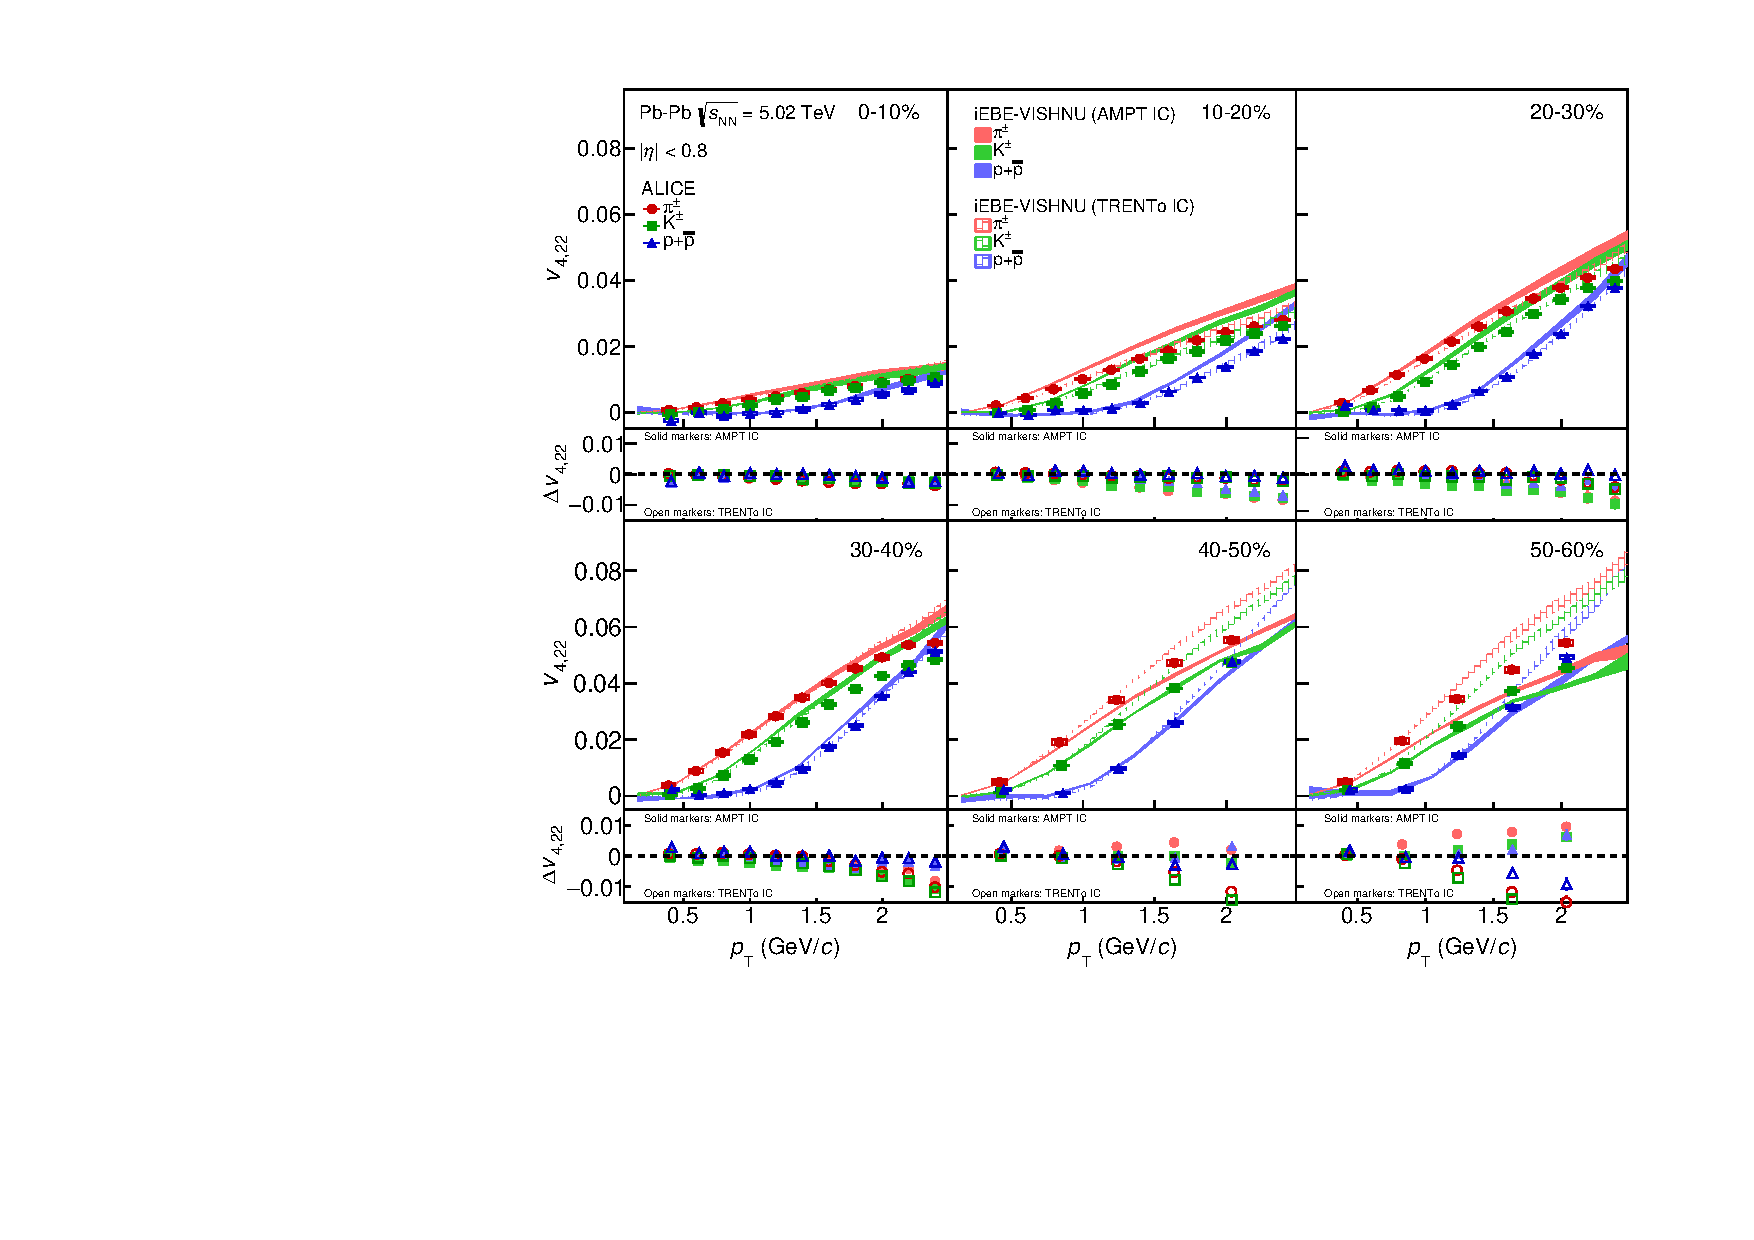
\includegraphics[scale=0.73]{figures/model/TrentoAndAMPT_v422_gap00_PID2.pdf}
%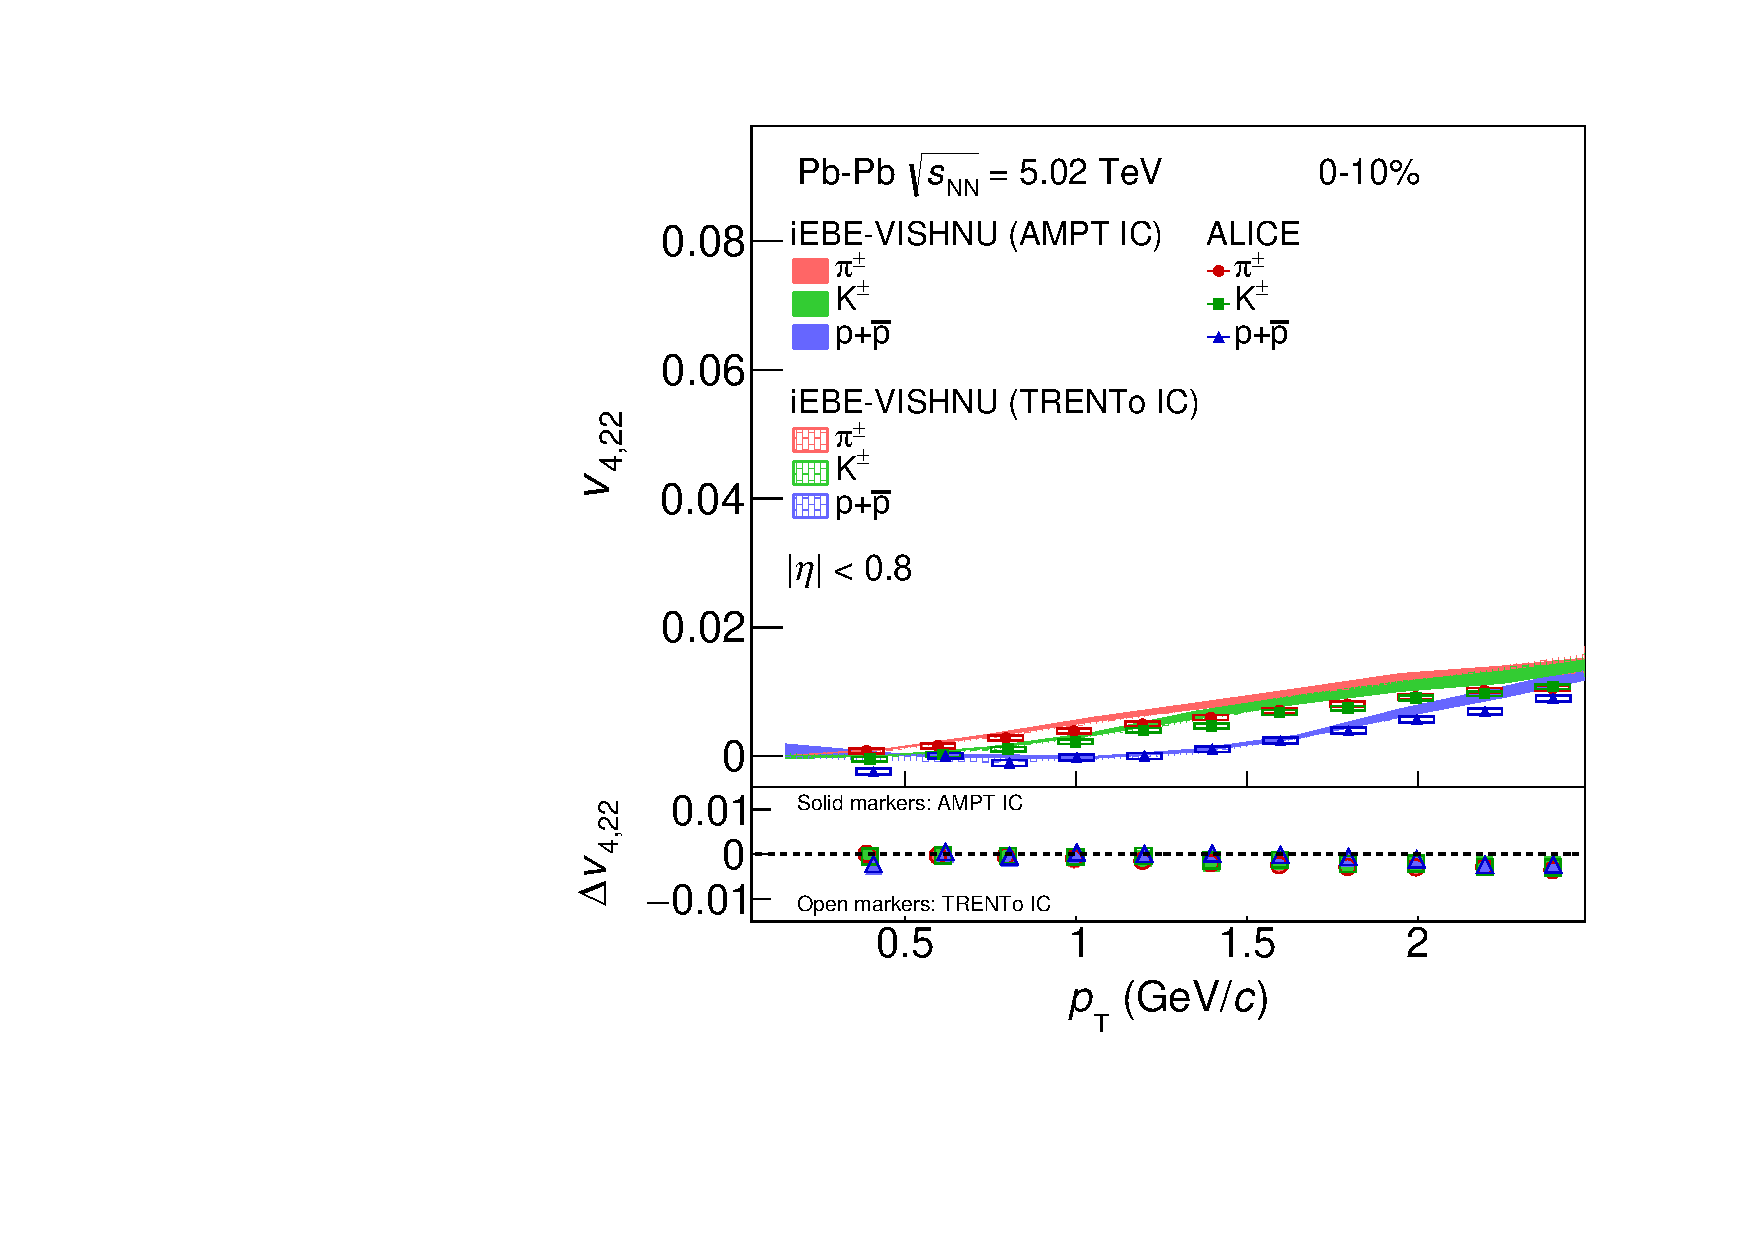
\includegraphics[scale=0.26]{figures/model/TrentoAndAMPT_v422_gap00_new_0-10_PID2.pdf}
%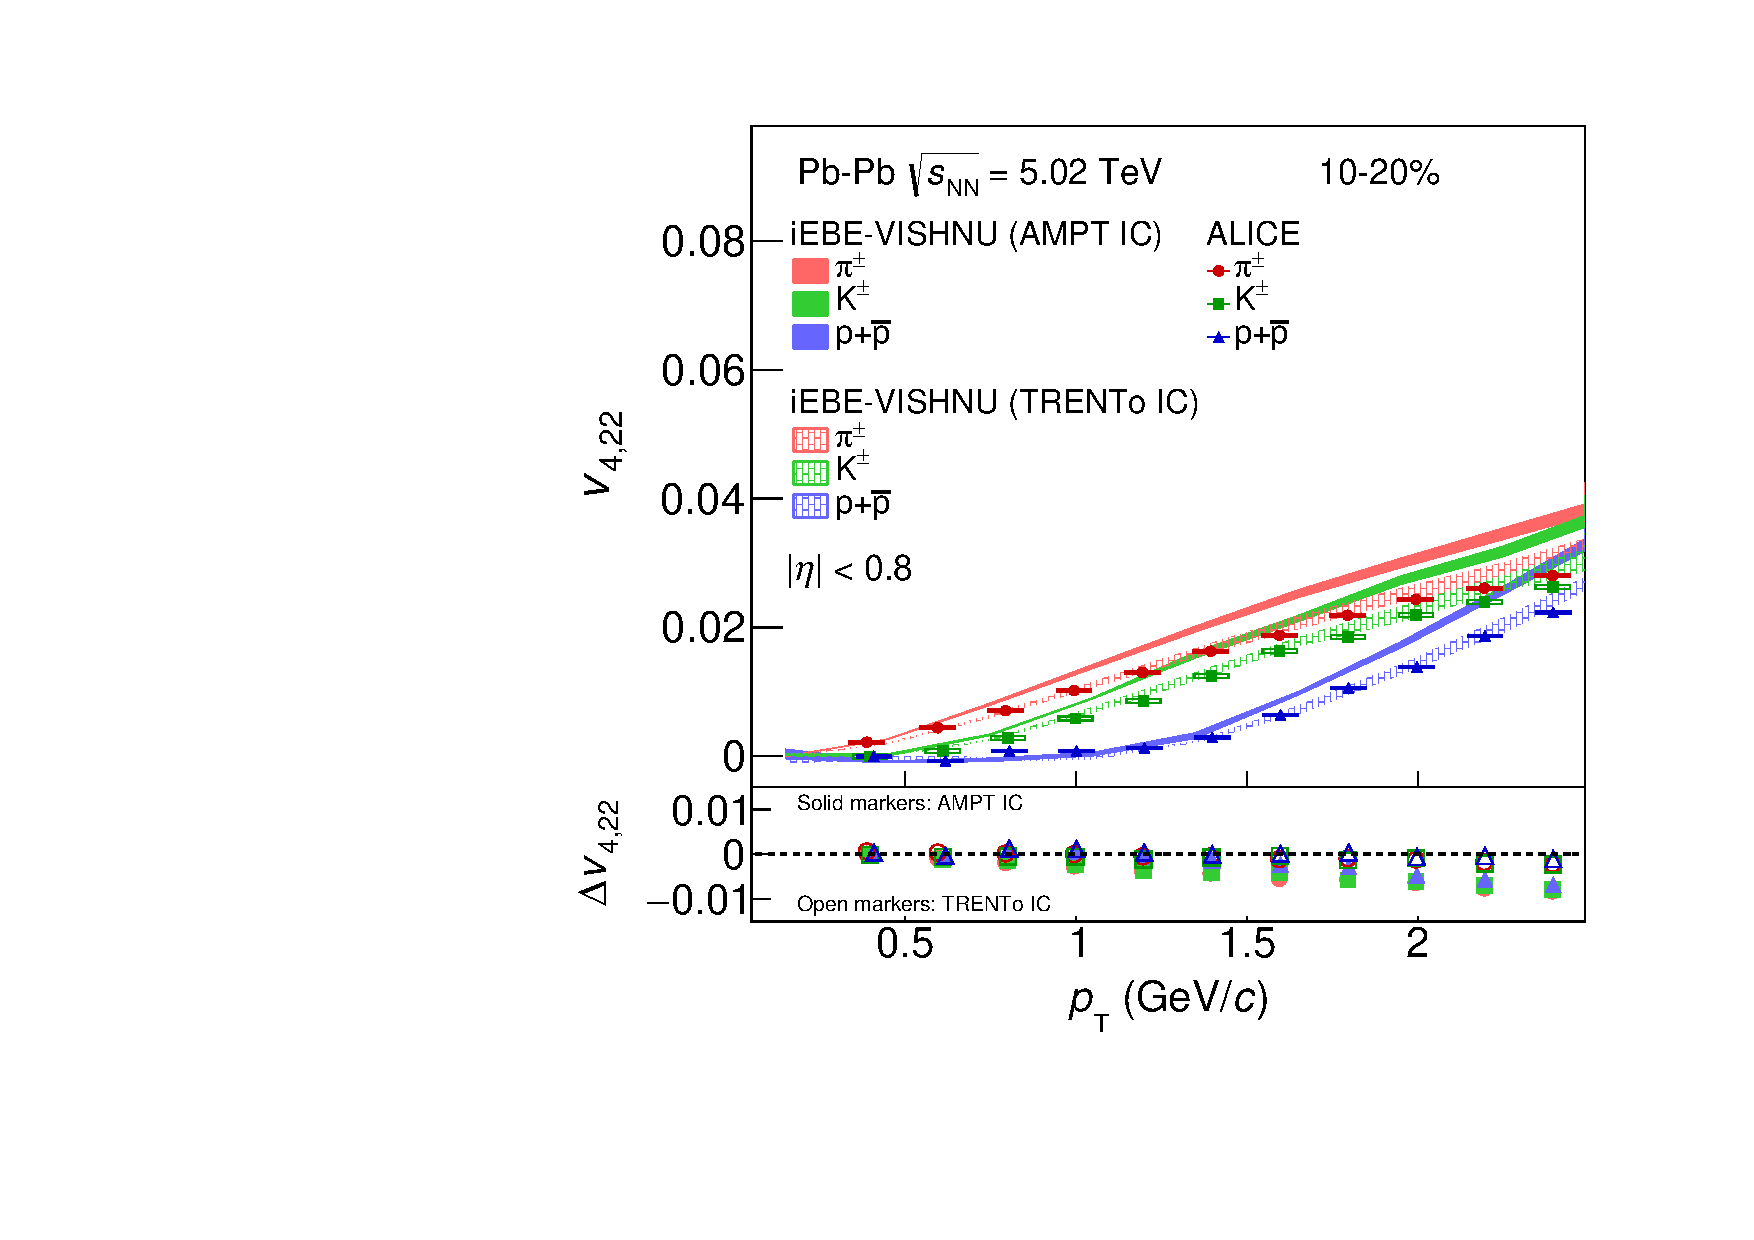
\includegraphics[scale=0.26]{figures/model/TrentoAndAMPT_v422_gap00_new_10-20_PID2.pdf}
%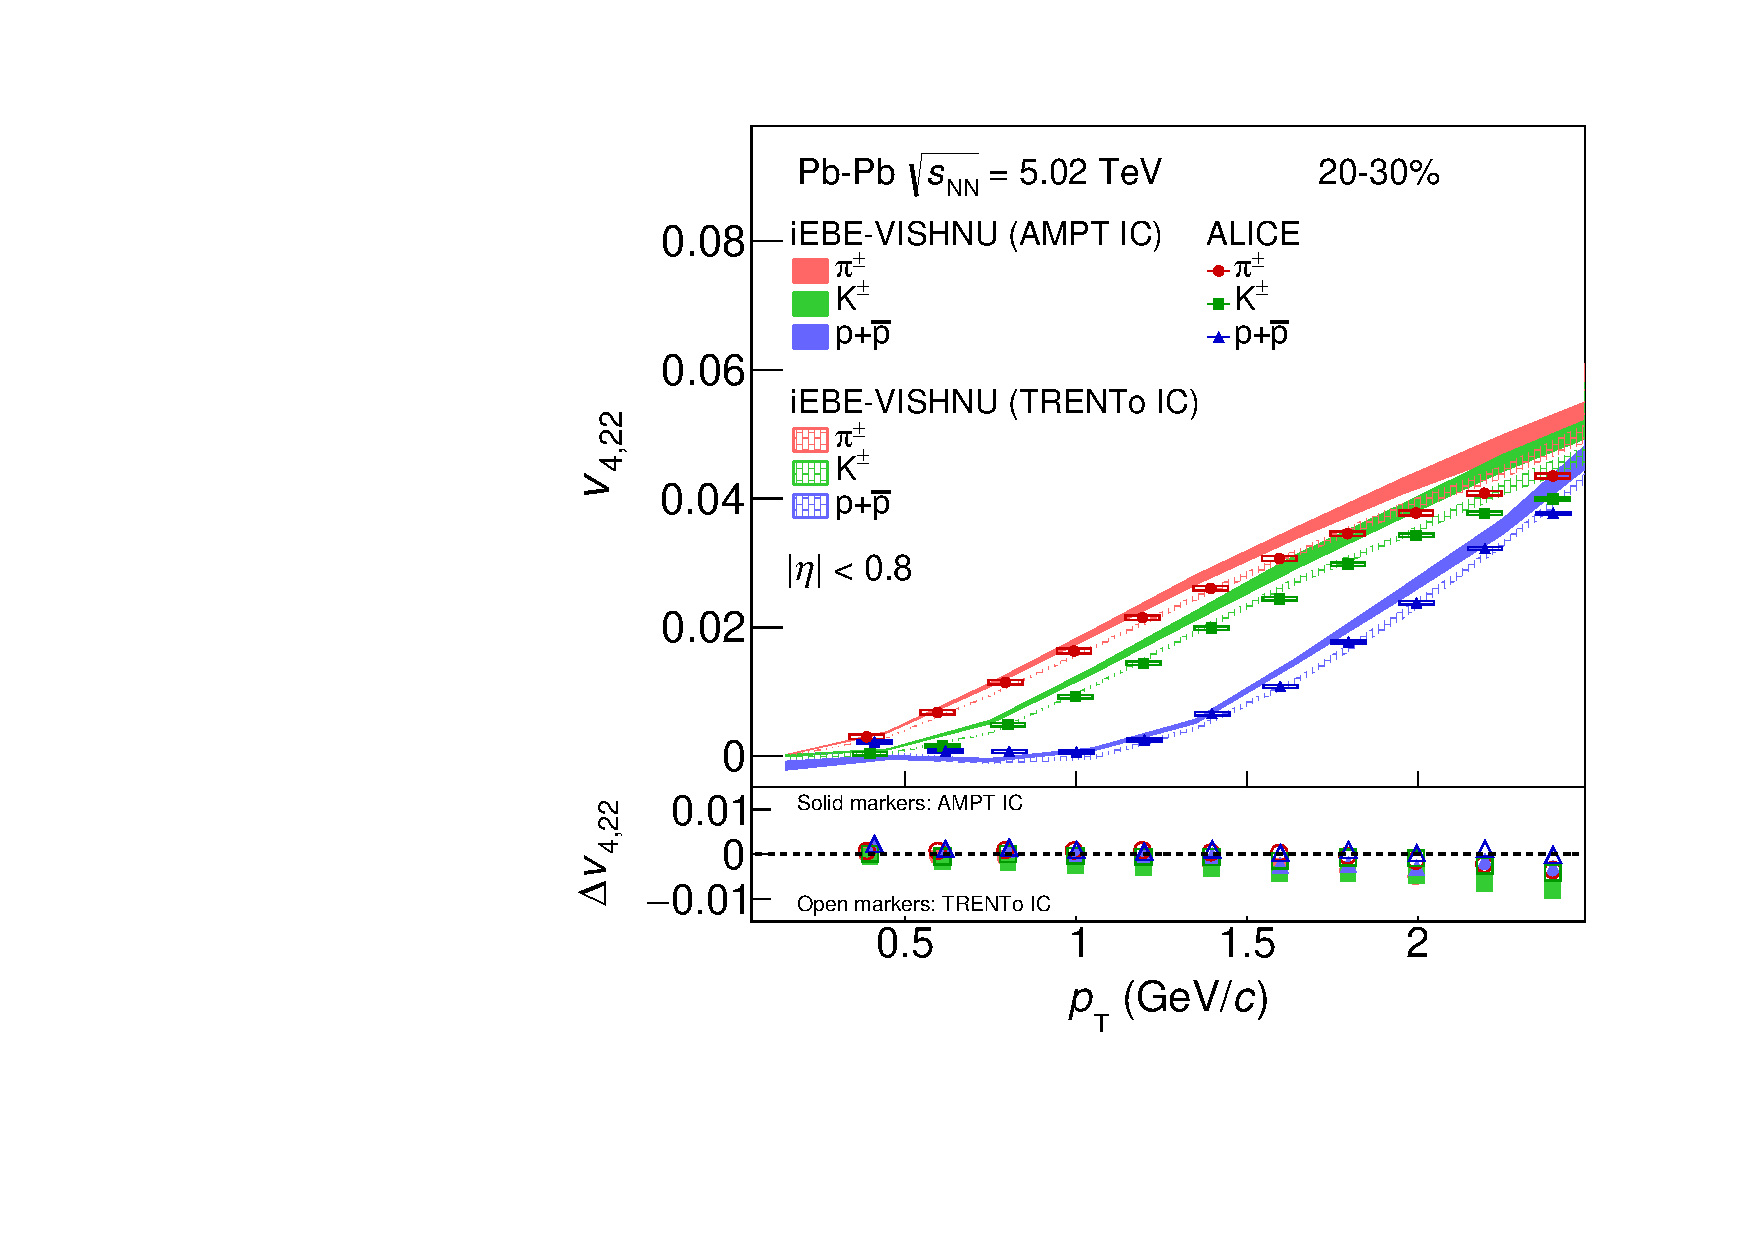
\includegraphics[scale=0.26]{figures/model/TrentoAndAMPT_v422_gap00_new_20-30_PID2.pdf}
%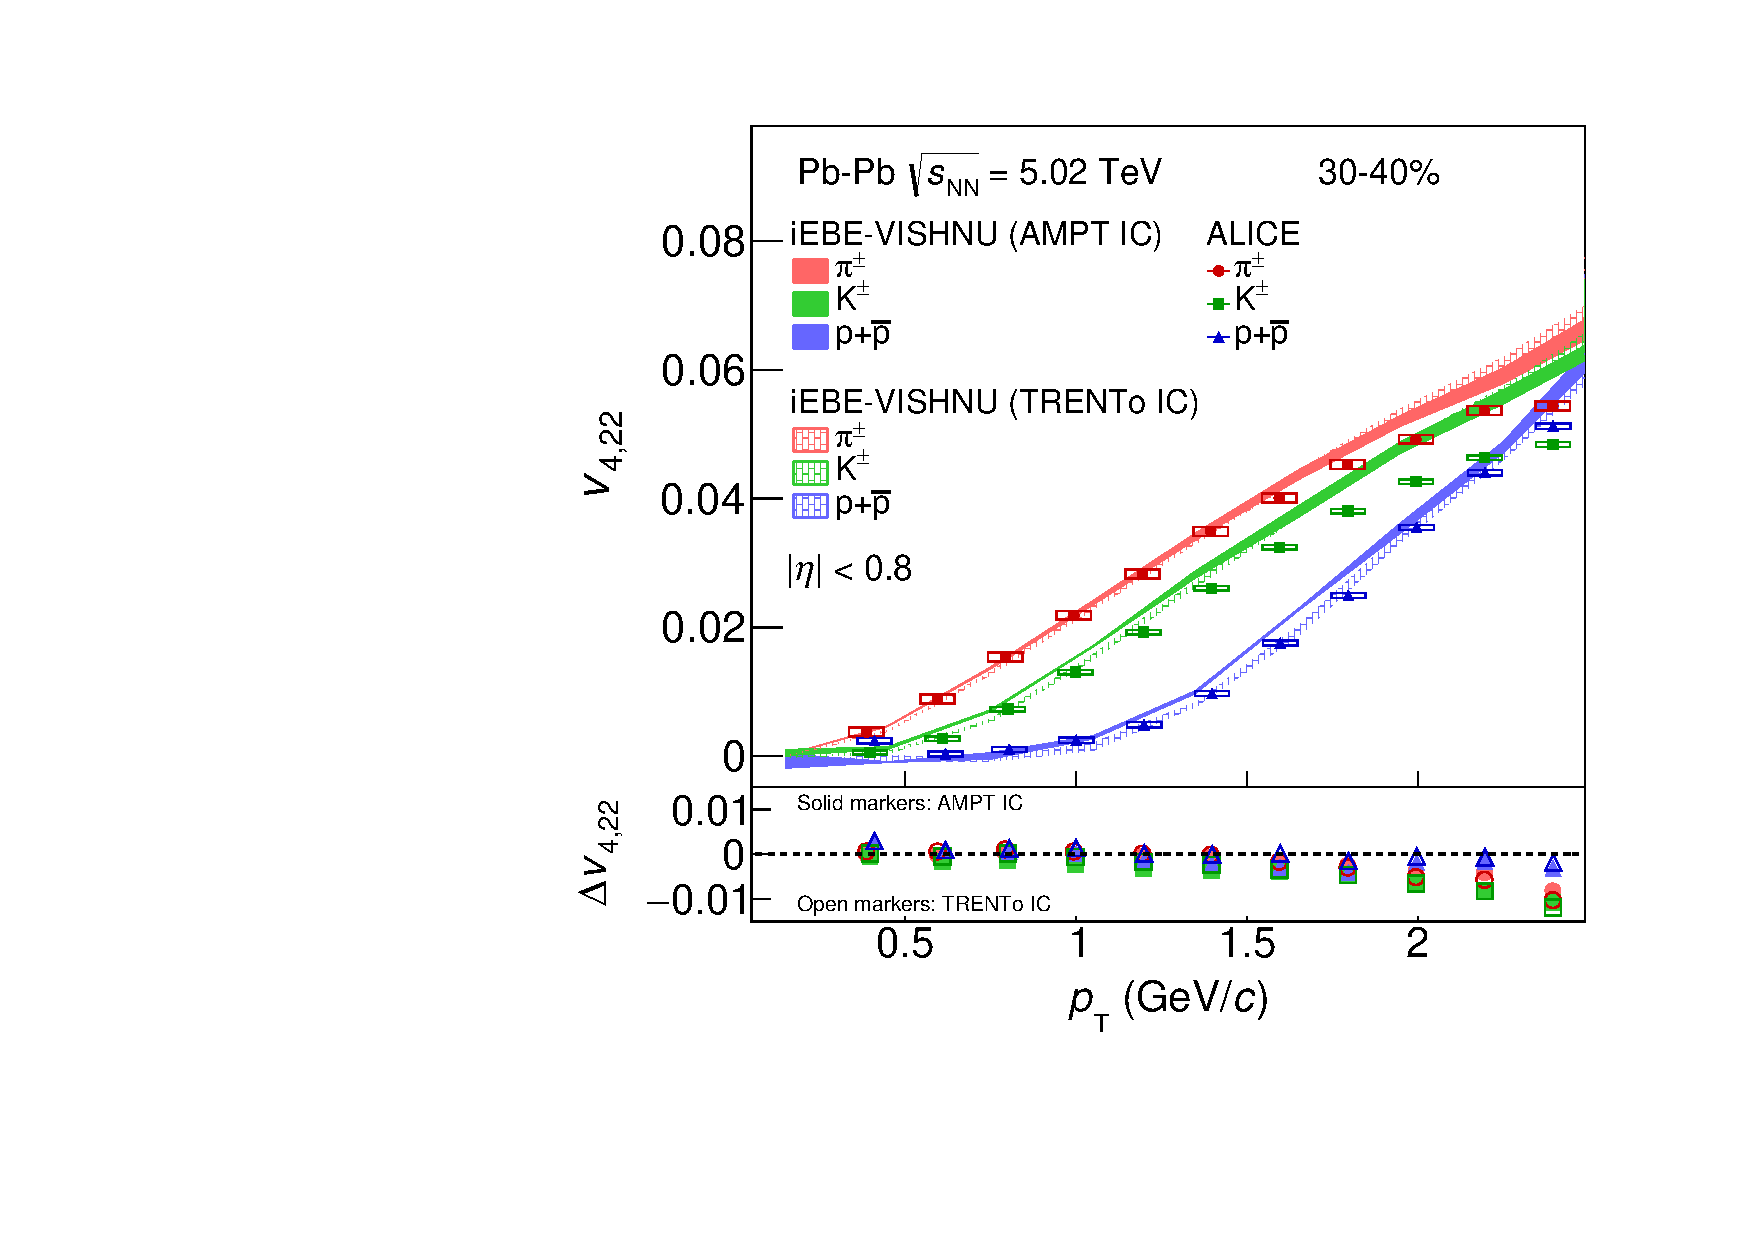
\includegraphics[scale=0.26]{figures/model/TrentoAndAMPT_v422_gap00_new_30-40_PID2.pdf}
%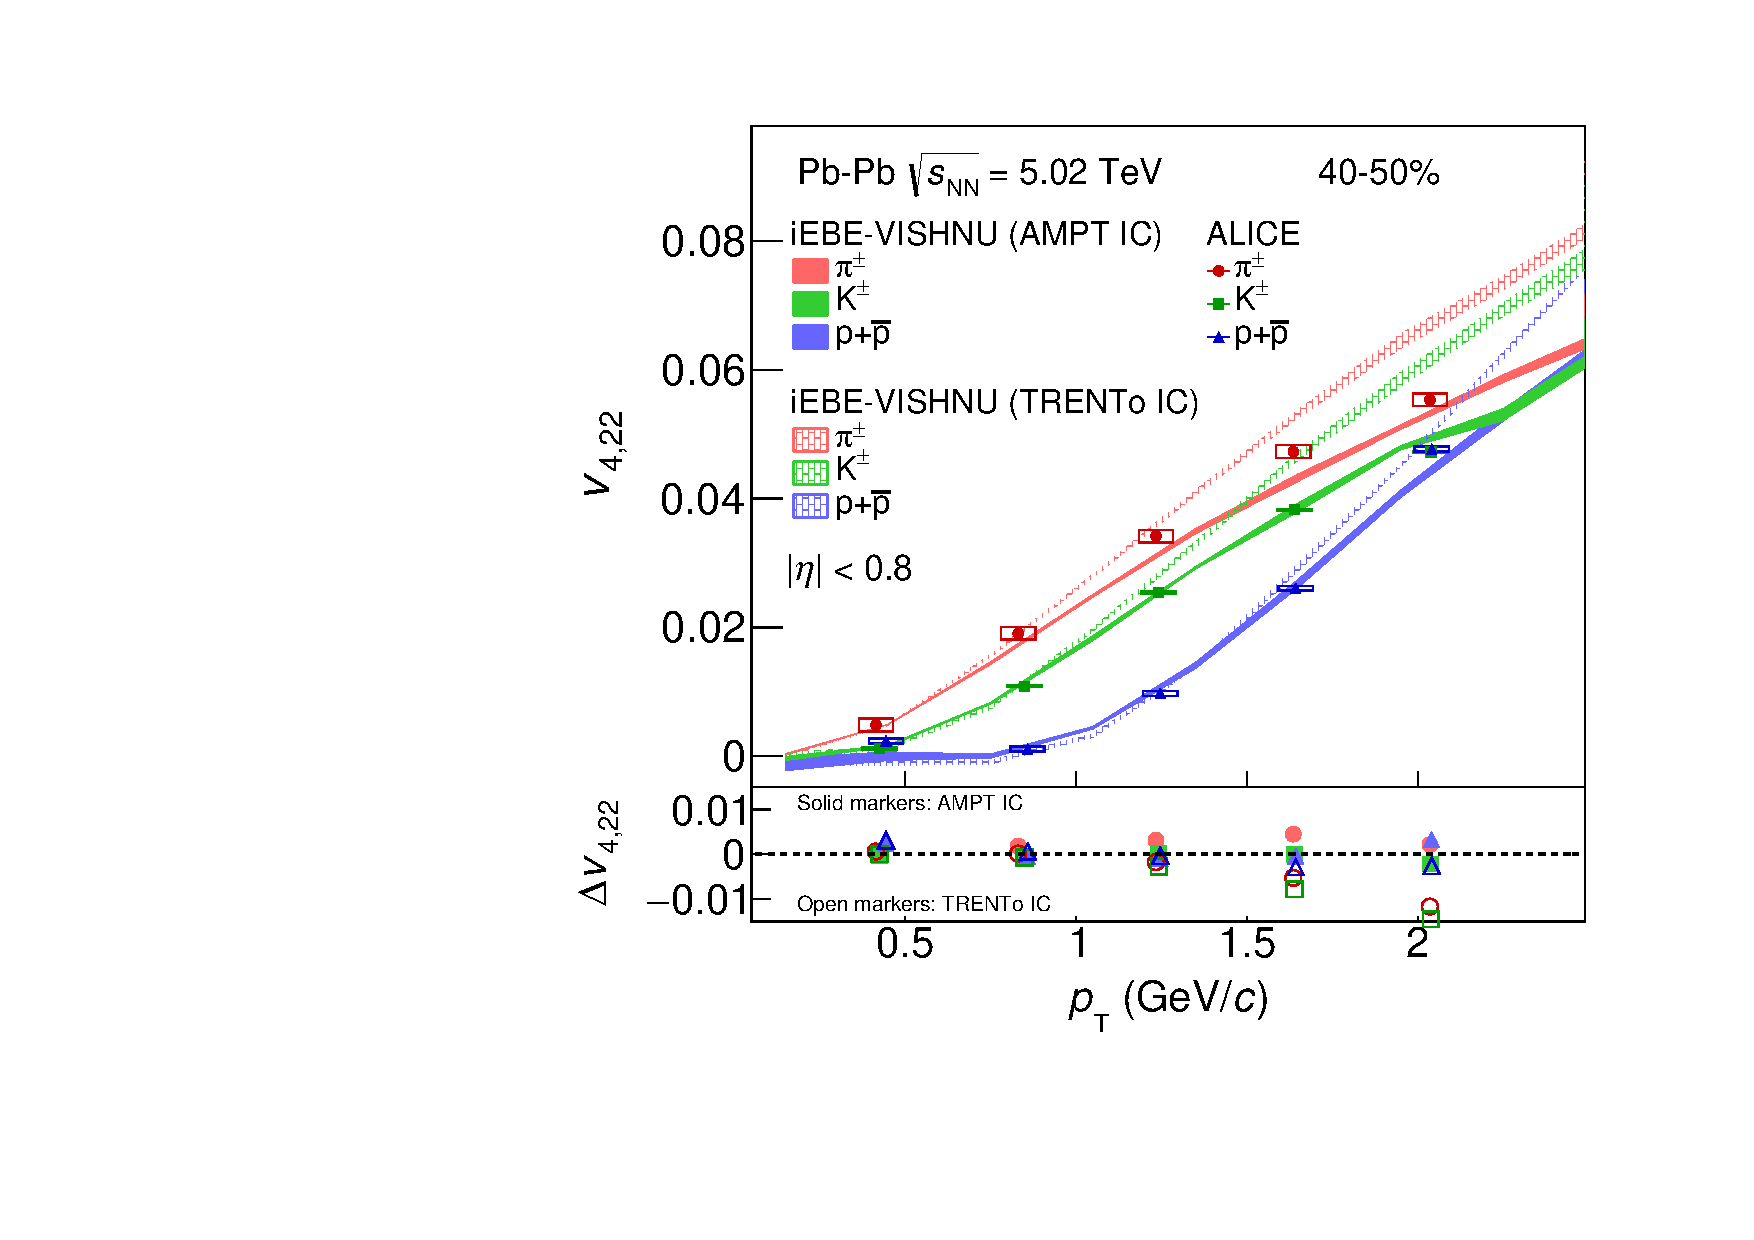
\includegraphics[scale=0.26]{figures/model/TrentoAndAMPT_v422_gap00_new_40-50_PID2.pdf}
%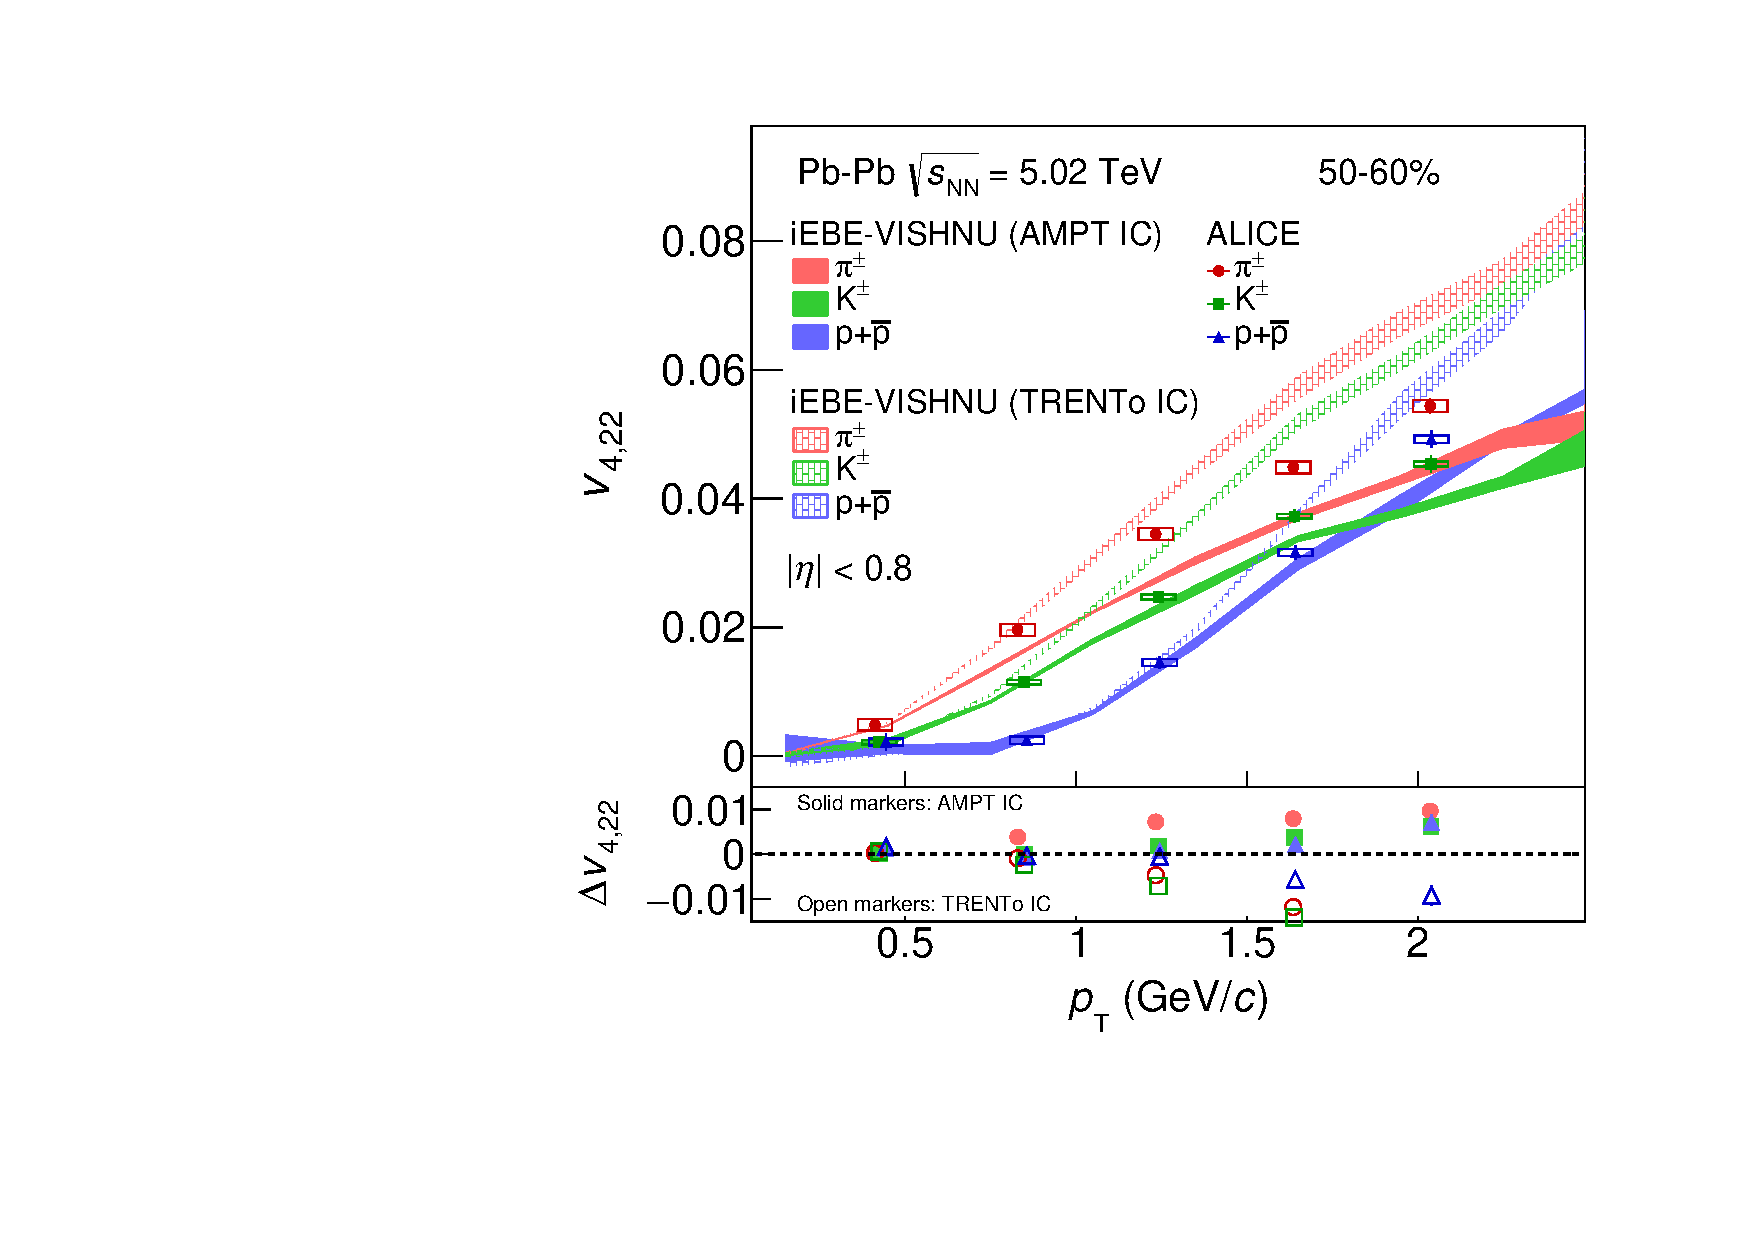
\includegraphics[scale=0.26]{figures/model/TrentoAndAMPT_v422_gap00_new_50-60_PID2.pdf}
\end{center}
\caption{The \pT-differential $v_{4,22}$ for different particle species in 10-20\% up to 50-60\% centrality intervals of Pb--Pb collisions at \sNN compared with iEBE-VISHNU hybrid models with two different sets of initial parameters: AMPT initial conditions ($\eta/s$= 0.08 and $\zeta/s$ = 0) shown in solid bands and TRENTo initial conditions ($\eta/s({\rm T})$ and $\zeta/s({\rm T})$) in hatched bands. The bottom panels show the difference between the measurements and each model.}
\label{v422_model}
\end{figure}


\begin{figure}[!htb]
\begin{center}
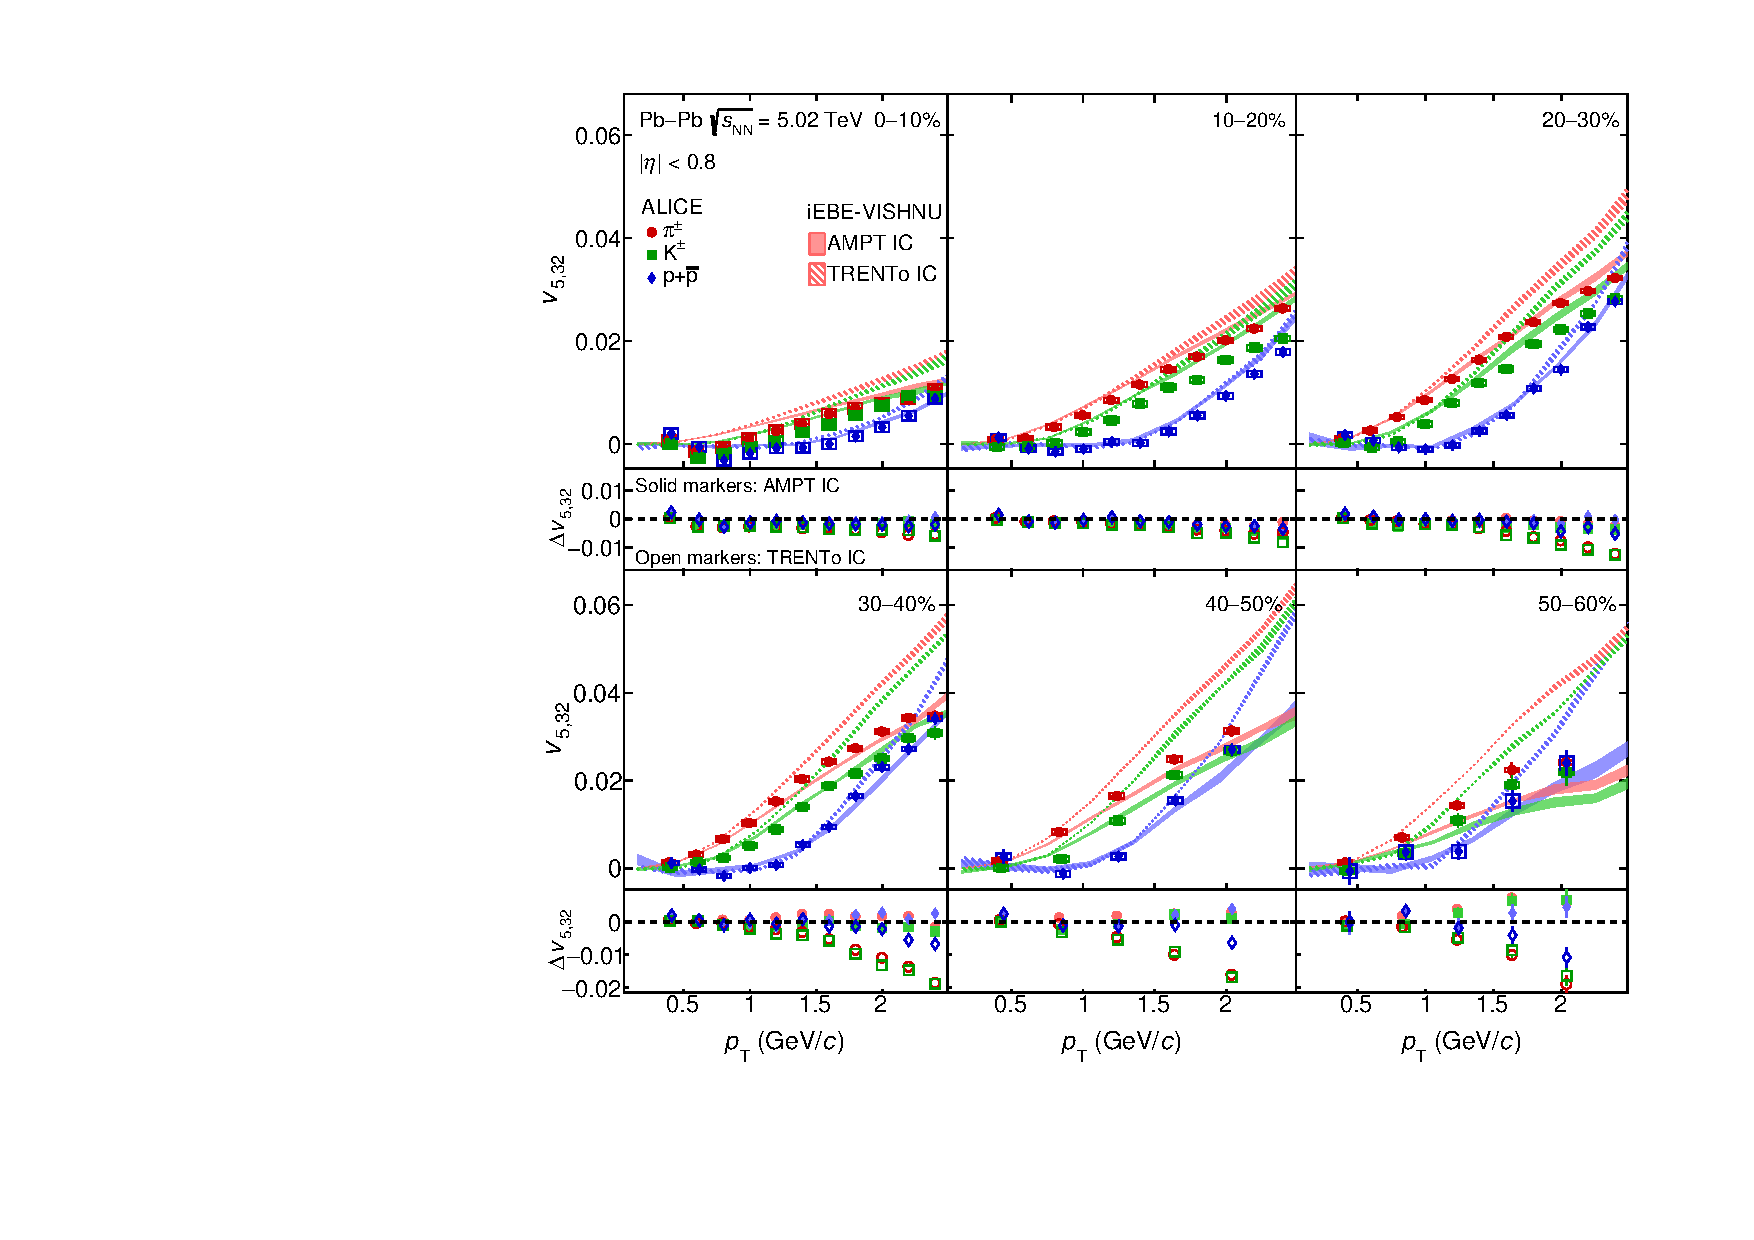
\includegraphics[scale=0.73]{figures/model/TrentoAndAMPT_v523_gap00_PID2.pdf}
%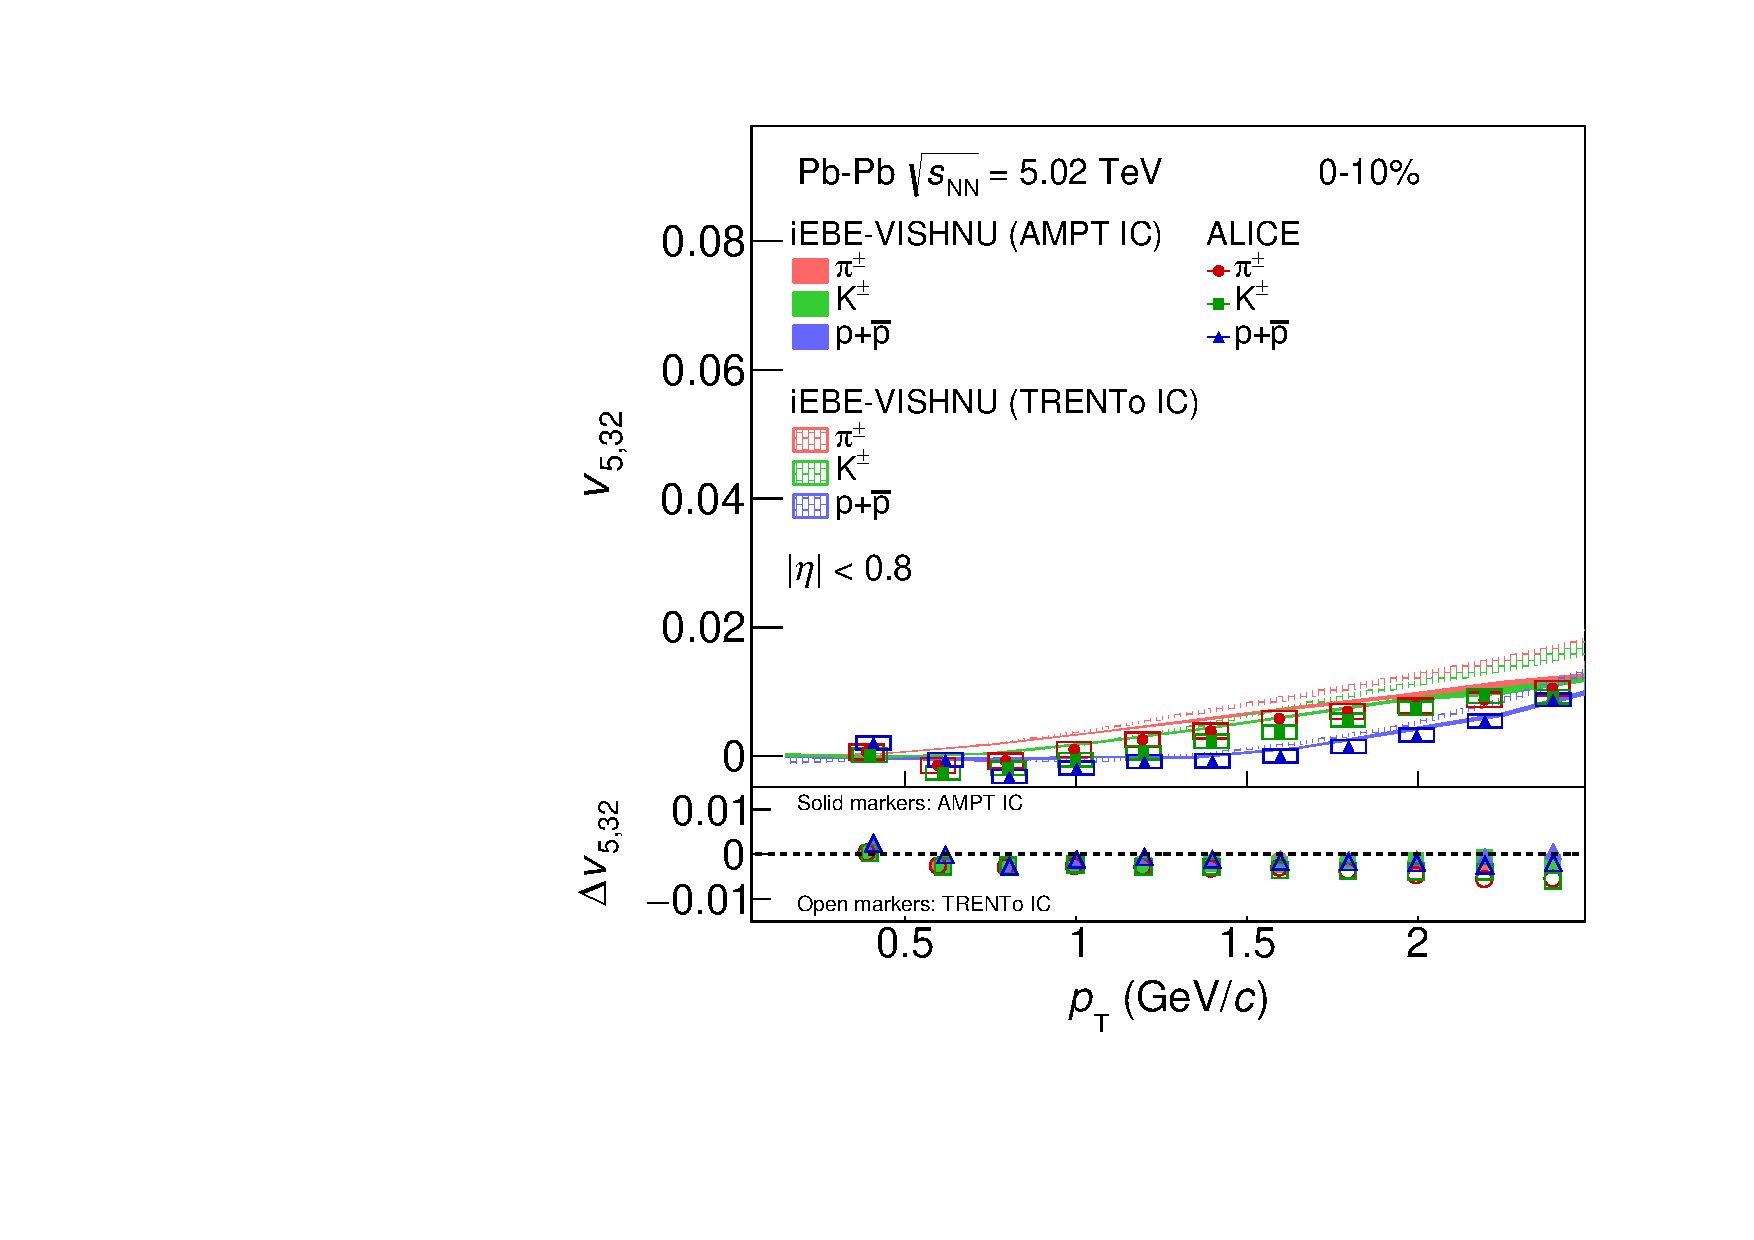
\includegraphics[scale=0.26]{figures/model/TrentoAndAMPT_v523_gap00_new_0-10_PID2.pdf}
%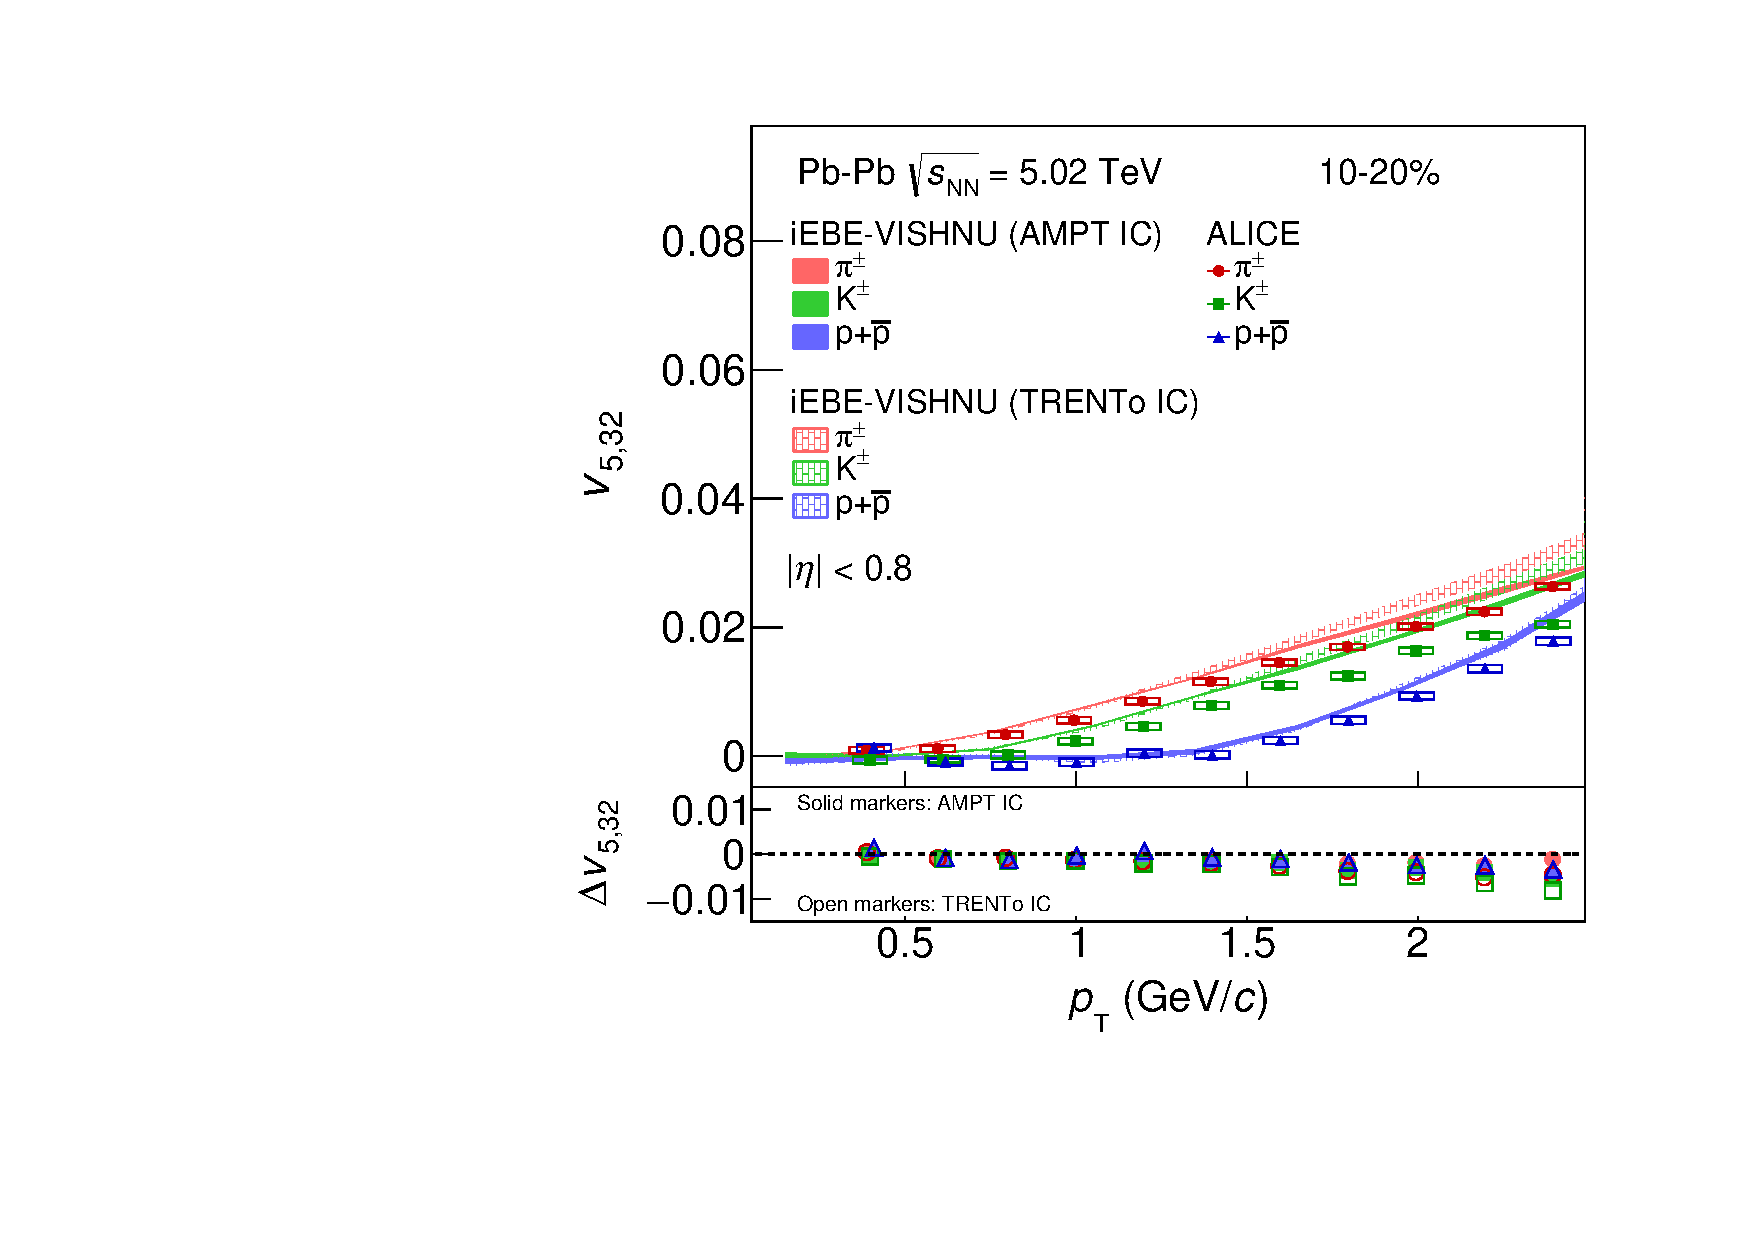
\includegraphics[scale=0.26]{figures/model/TrentoAndAMPT_v523_gap00_new_10-20_PID2.pdf}
%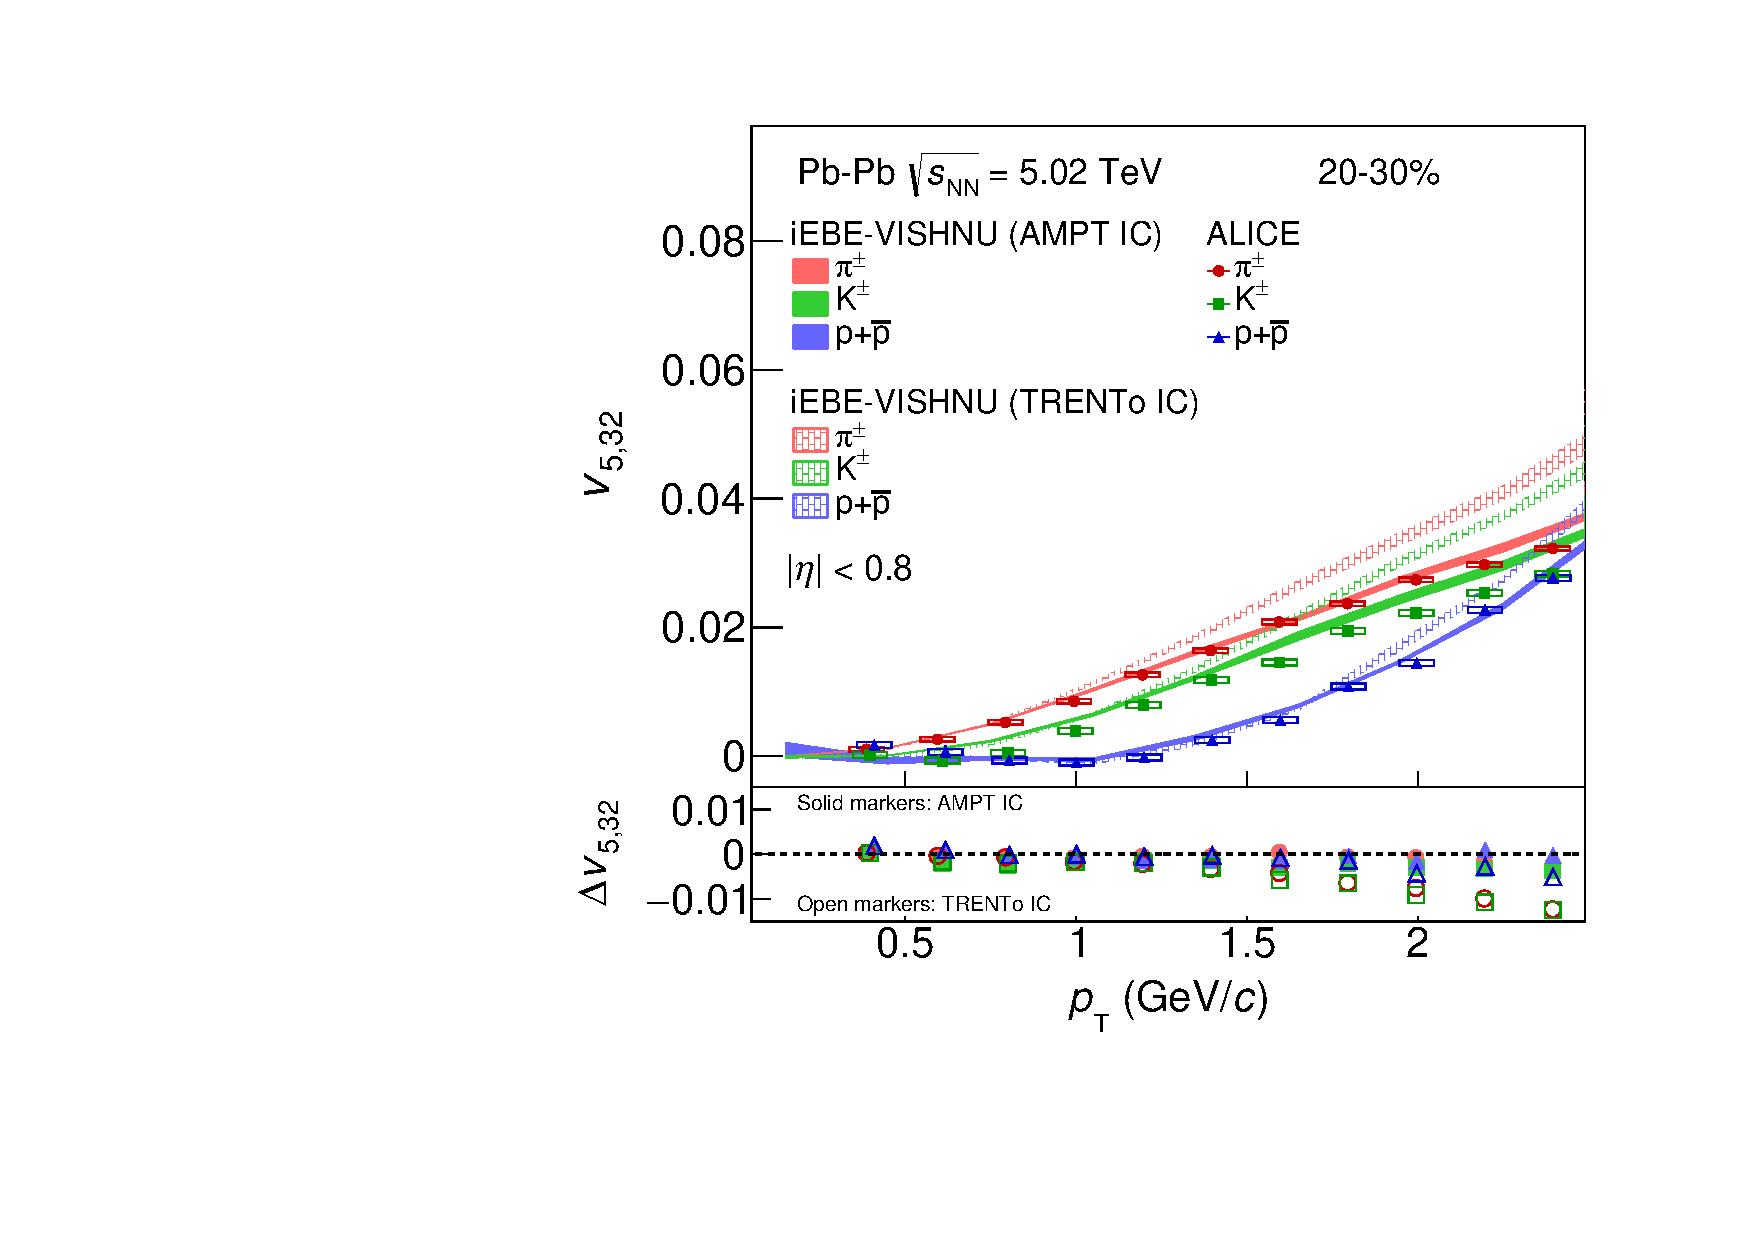
\includegraphics[scale=0.26]{figures/model/TrentoAndAMPT_v523_gap00_new_20-30_PID2.pdf}
%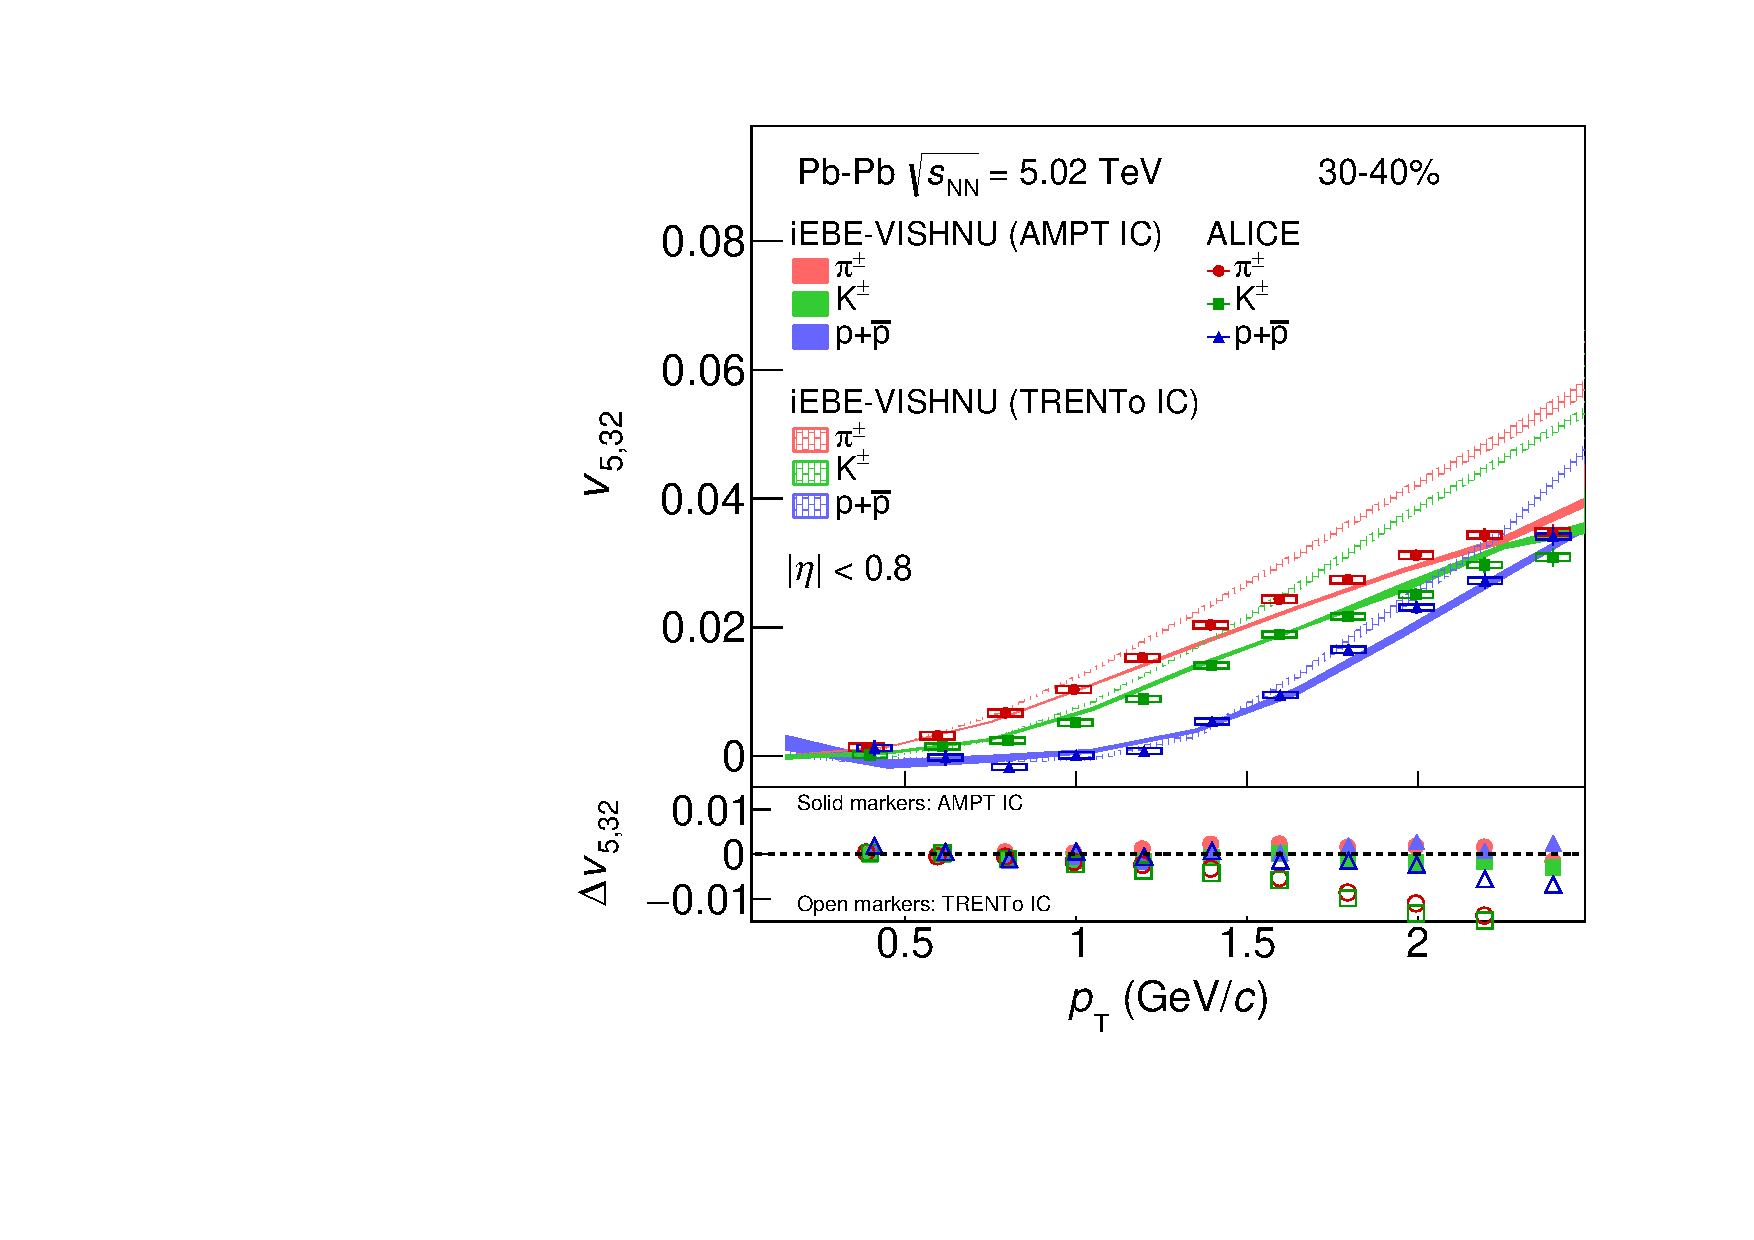
\includegraphics[scale=0.26]{figures/model/TrentoAndAMPT_v523_gap00_new_30-40_PID2.pdf}
%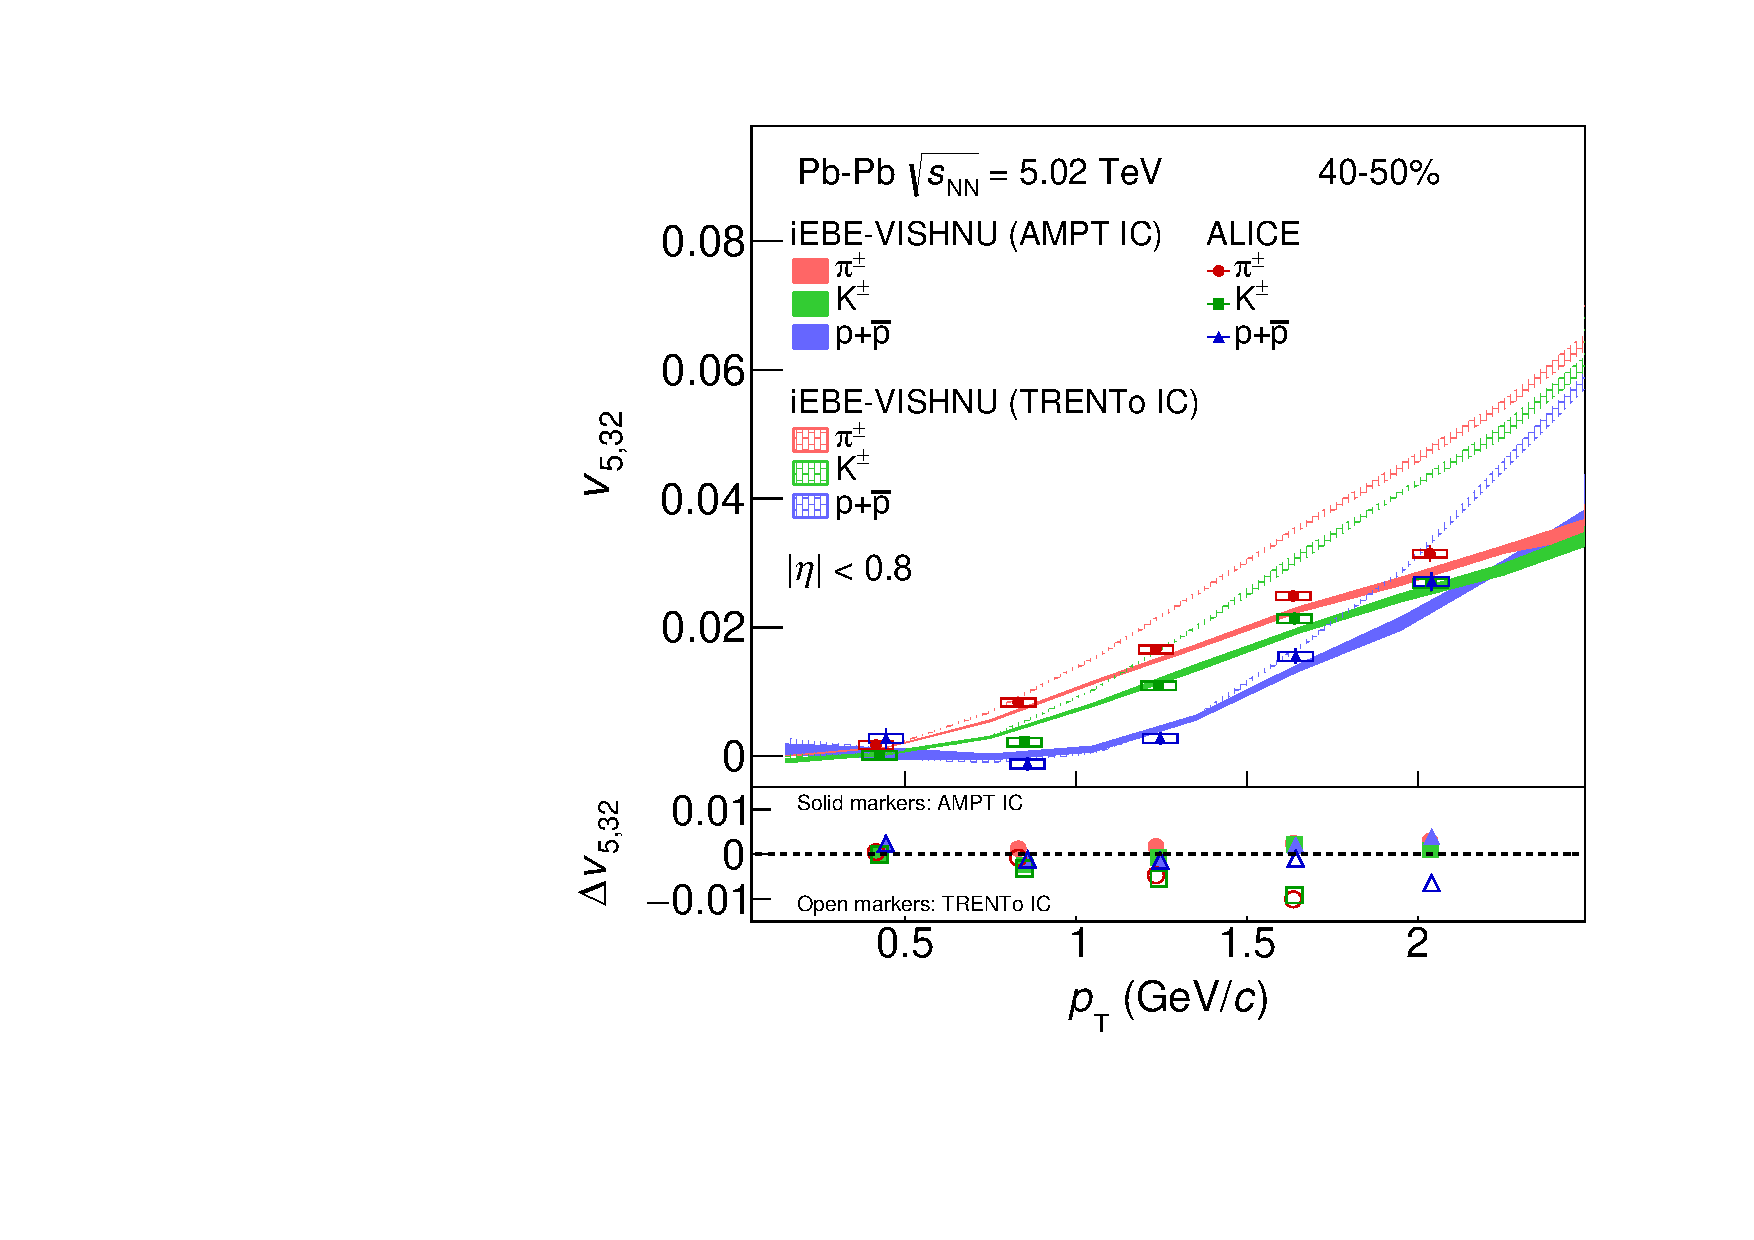
\includegraphics[scale=0.26]{figures/model/TrentoAndAMPT_v523_gap00_new_40-50_PID2.pdf}
%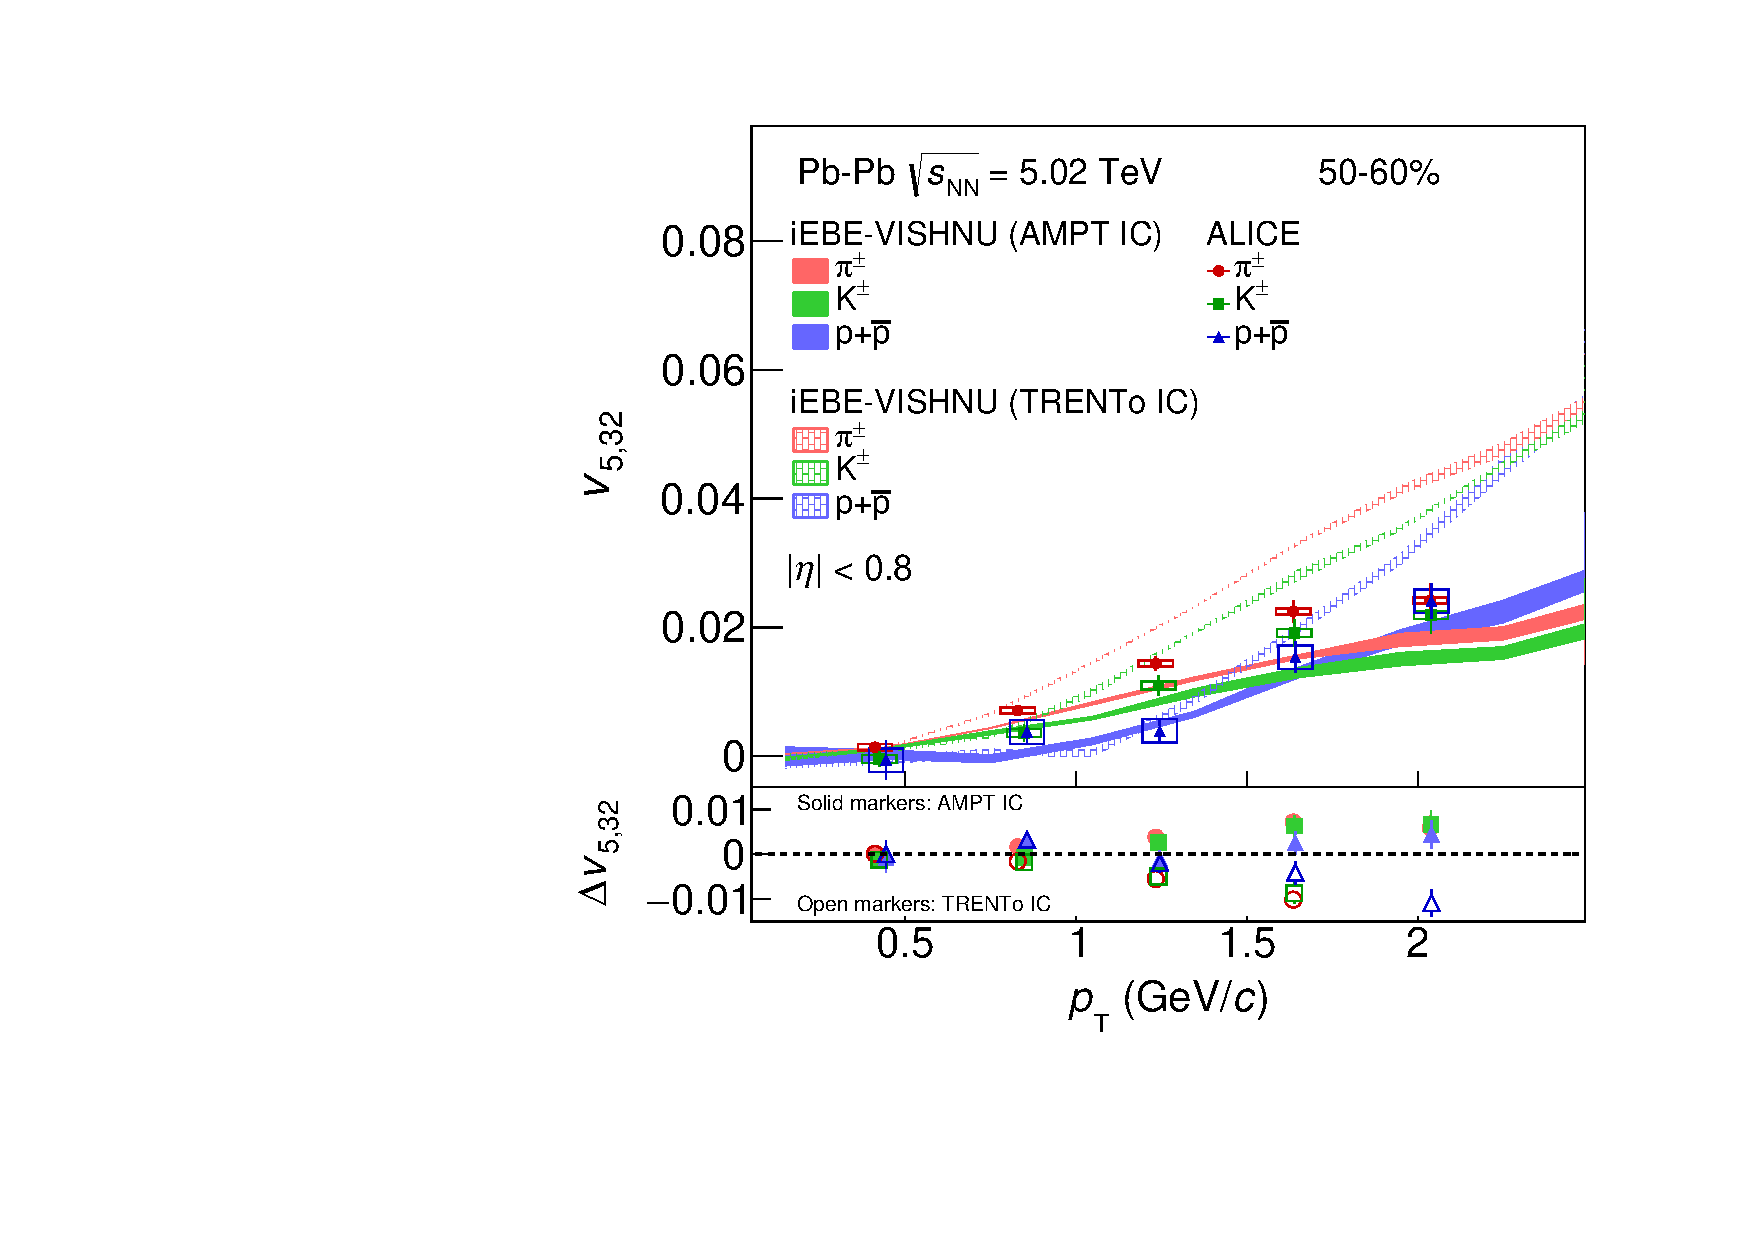
\includegraphics[scale=0.26]{figures/model/TrentoAndAMPT_v523_gap00_new_50-60_PID2.pdf}
\end{center}
\caption{The \pT-differential $v_{5,32}$ for different particle species in 10-20\% up to 50-60\% centrality intervals of Pb--Pb collisions at \sNN compared with iEBE-VISHNU hybrid models with two different sets of initial parameters: AMPT initial conditions ($\eta/s$= 0.08 and $\zeta/s$ = 0) shown in solid bands and TRENTo initial conditions ($\eta/s({\rm T})$ and $\zeta/s({\rm T})$) in hatched bands. The bottom panels show the difference between the measurements and each model.}
\label{v523_model}
\end{figure}

\begin{figure}[!htb]
\begin{center}
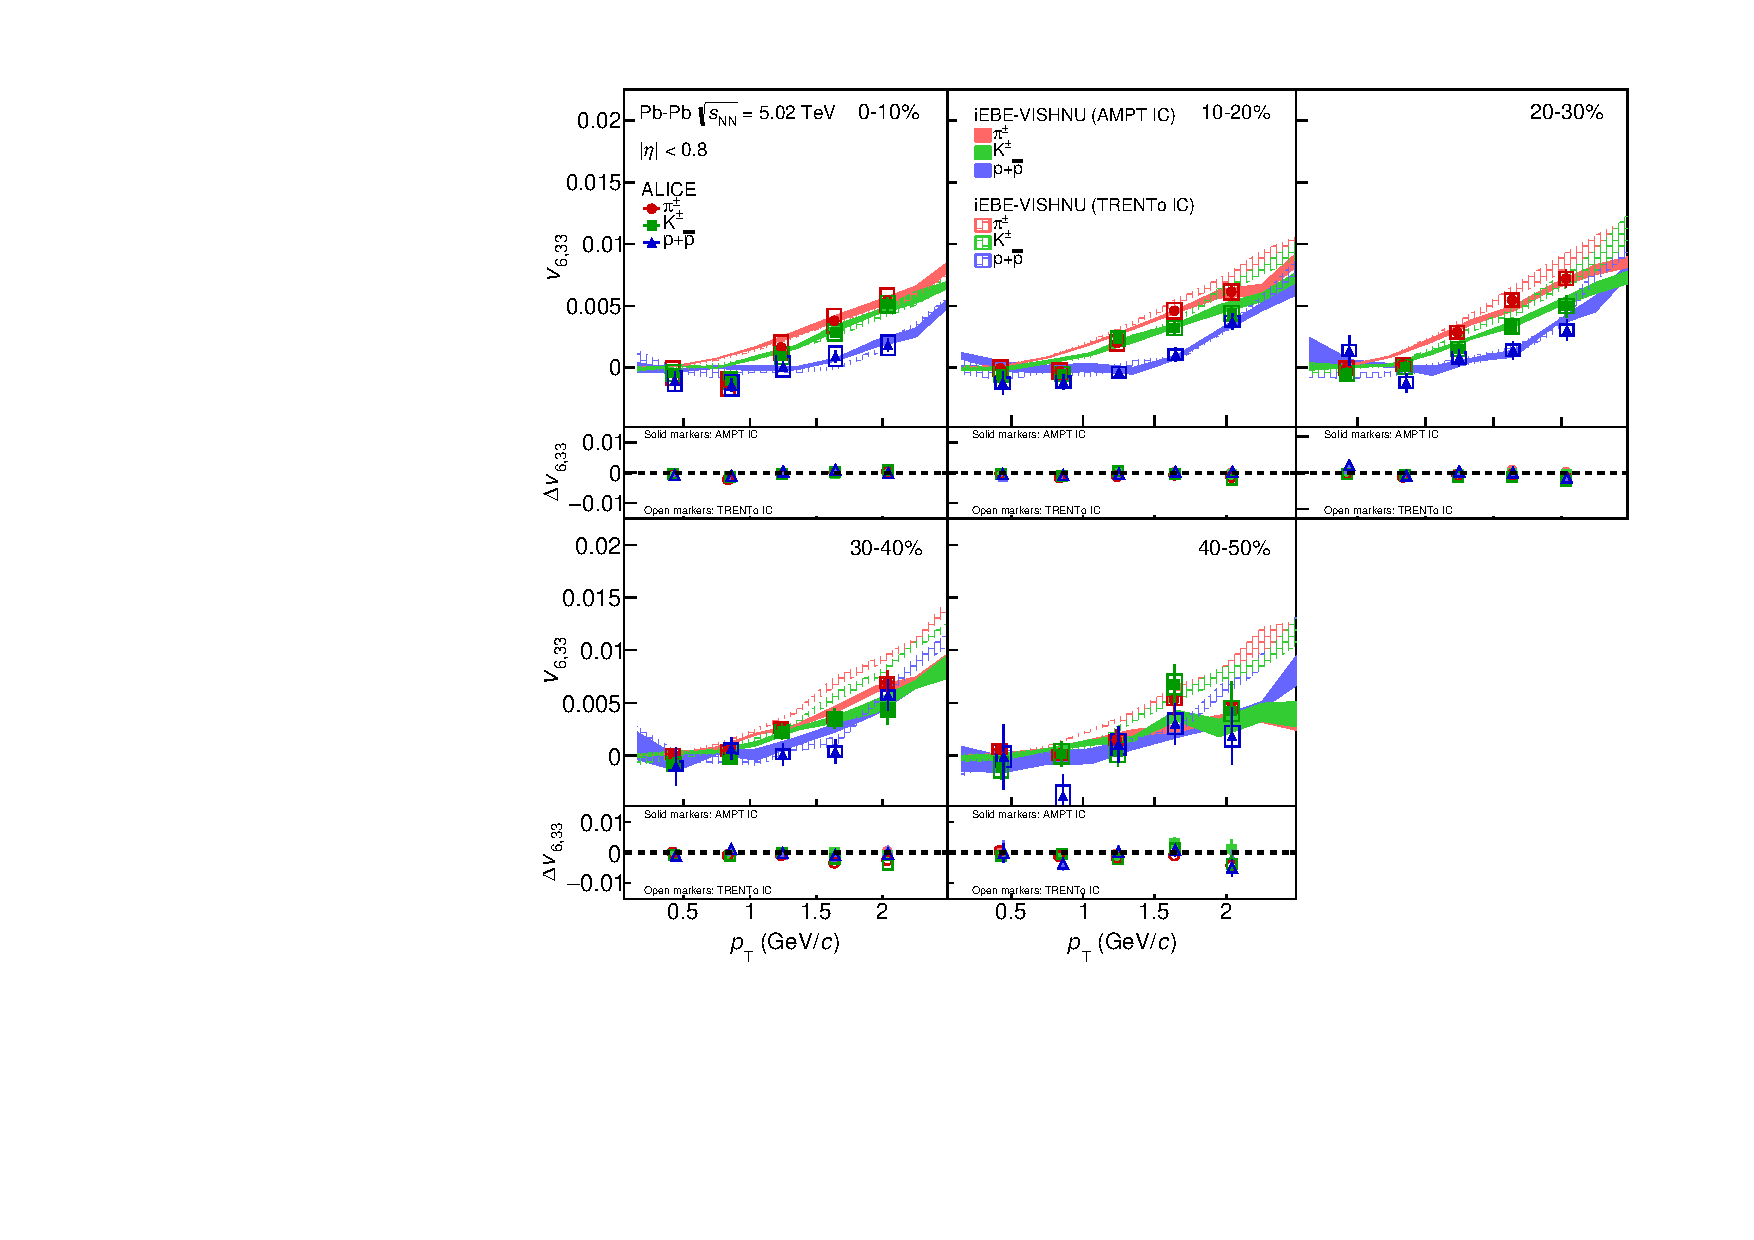
\includegraphics[scale=0.73]{figures/model/TrentoAndAMPT_v633_gap00_PID2.pdf}
%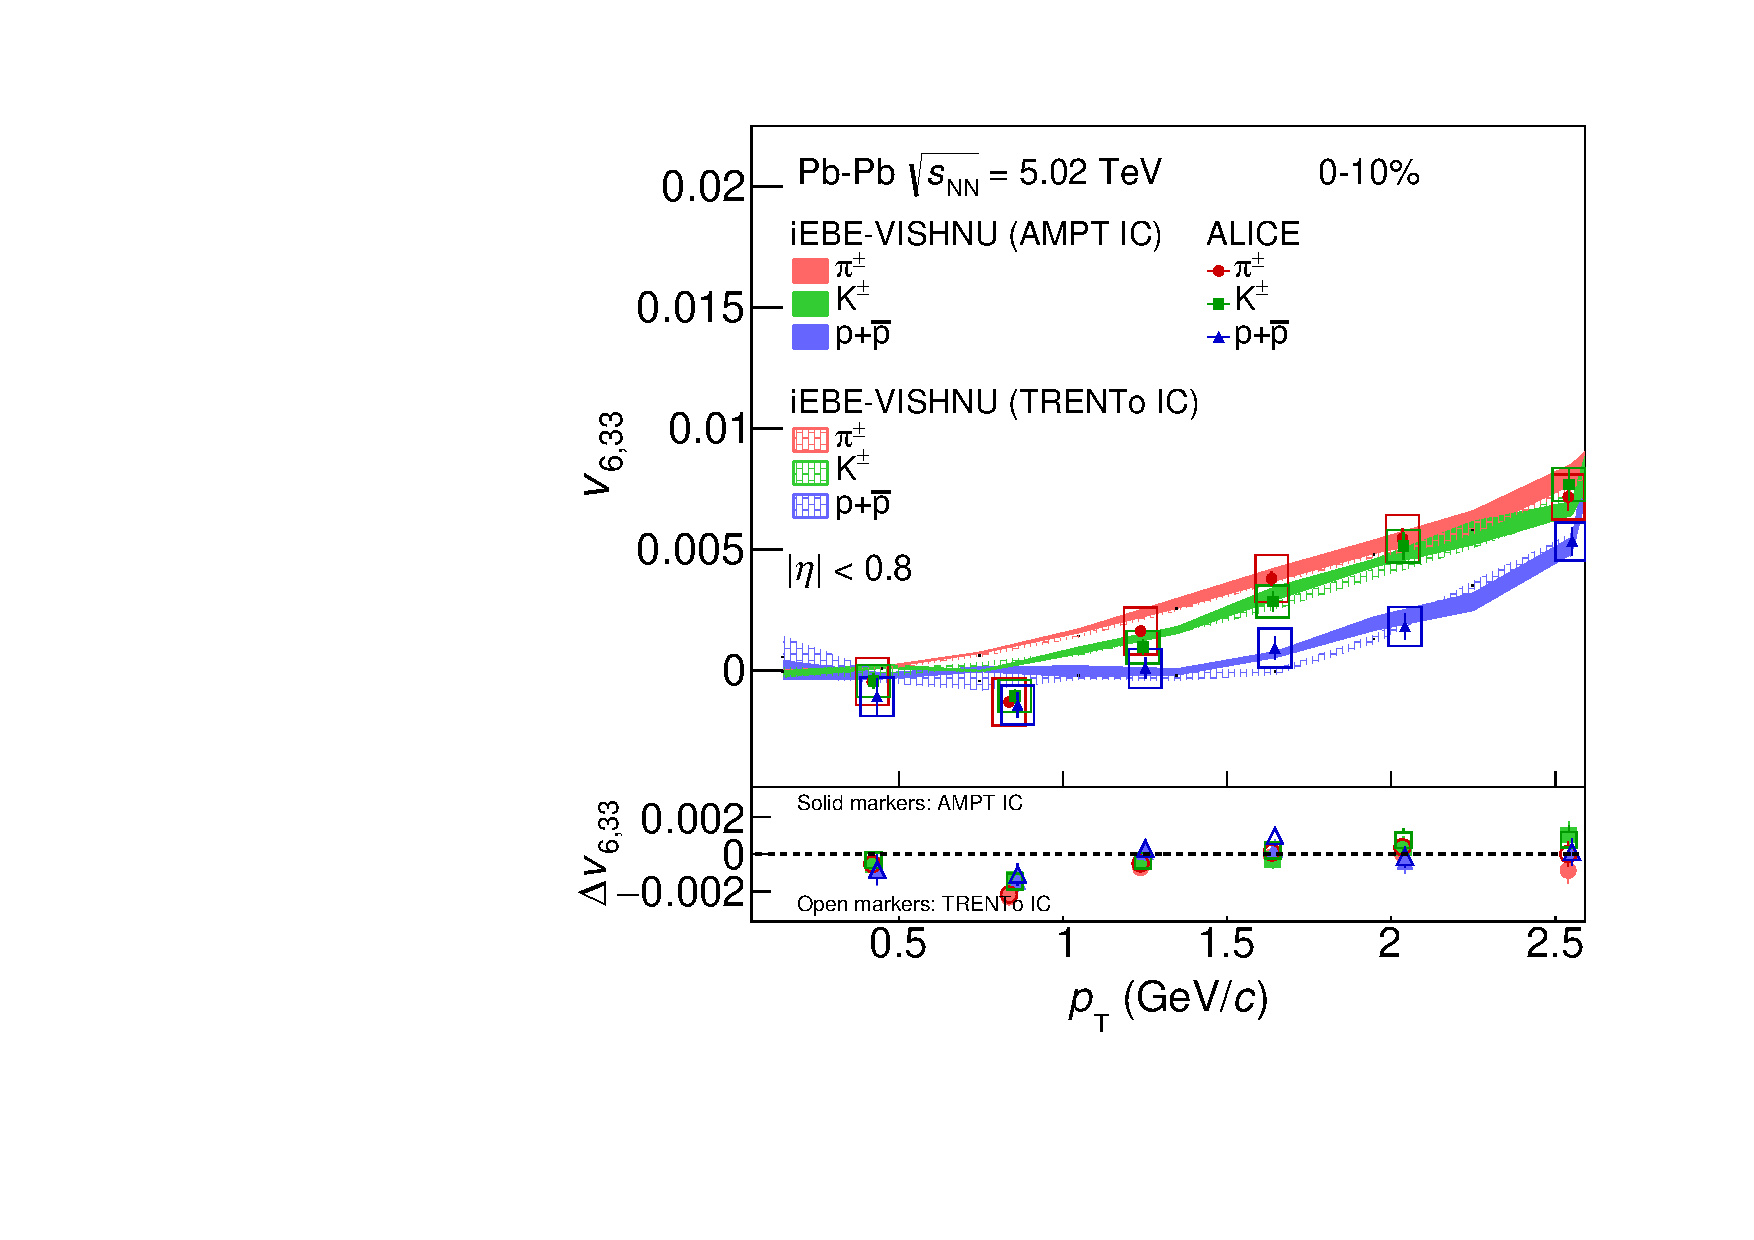
\includegraphics[scale=0.26]{figures/model/TrentoAndAMPT_v633_gap00_new_0-10_PID2.pdf}
%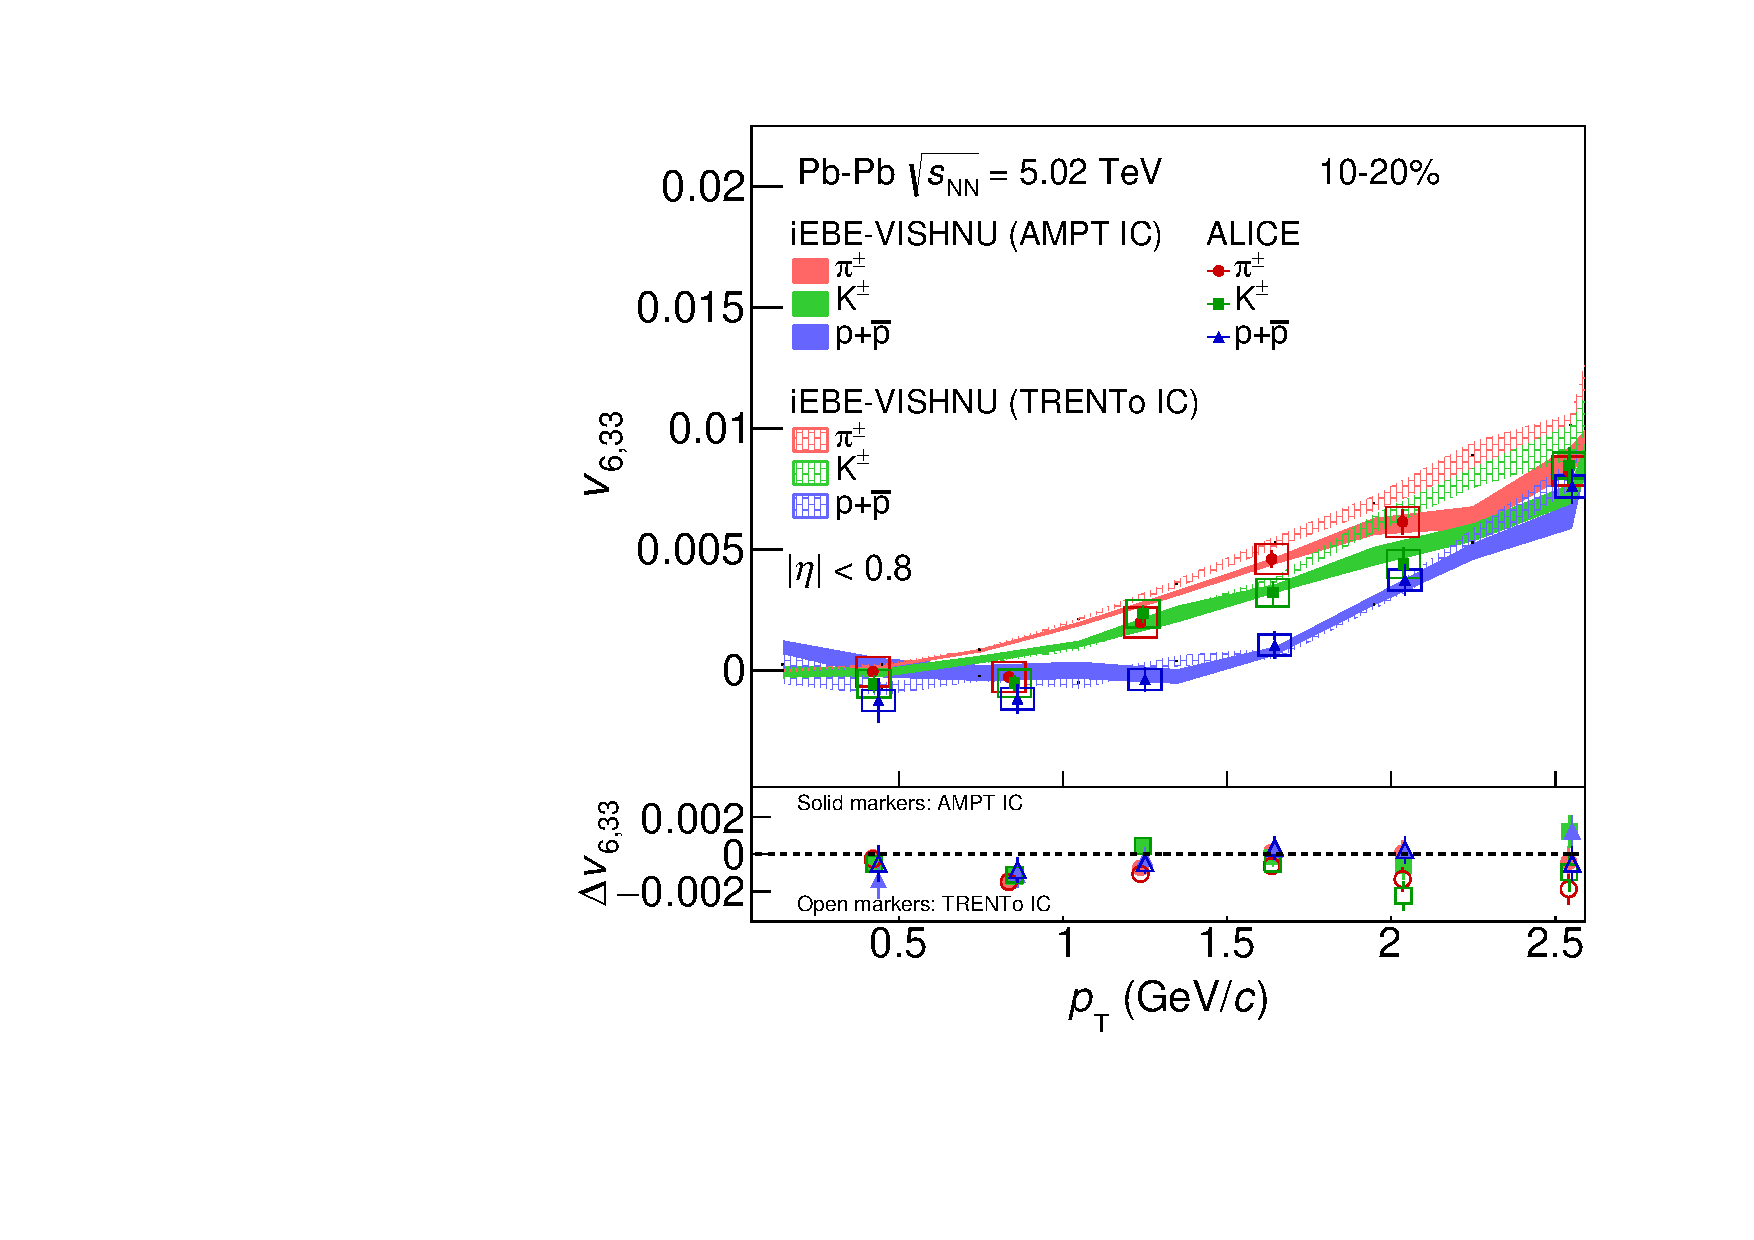
\includegraphics[scale=0.26]{figures/model/TrentoAndAMPT_v633_gap00_new_10-20_PID2.pdf}
%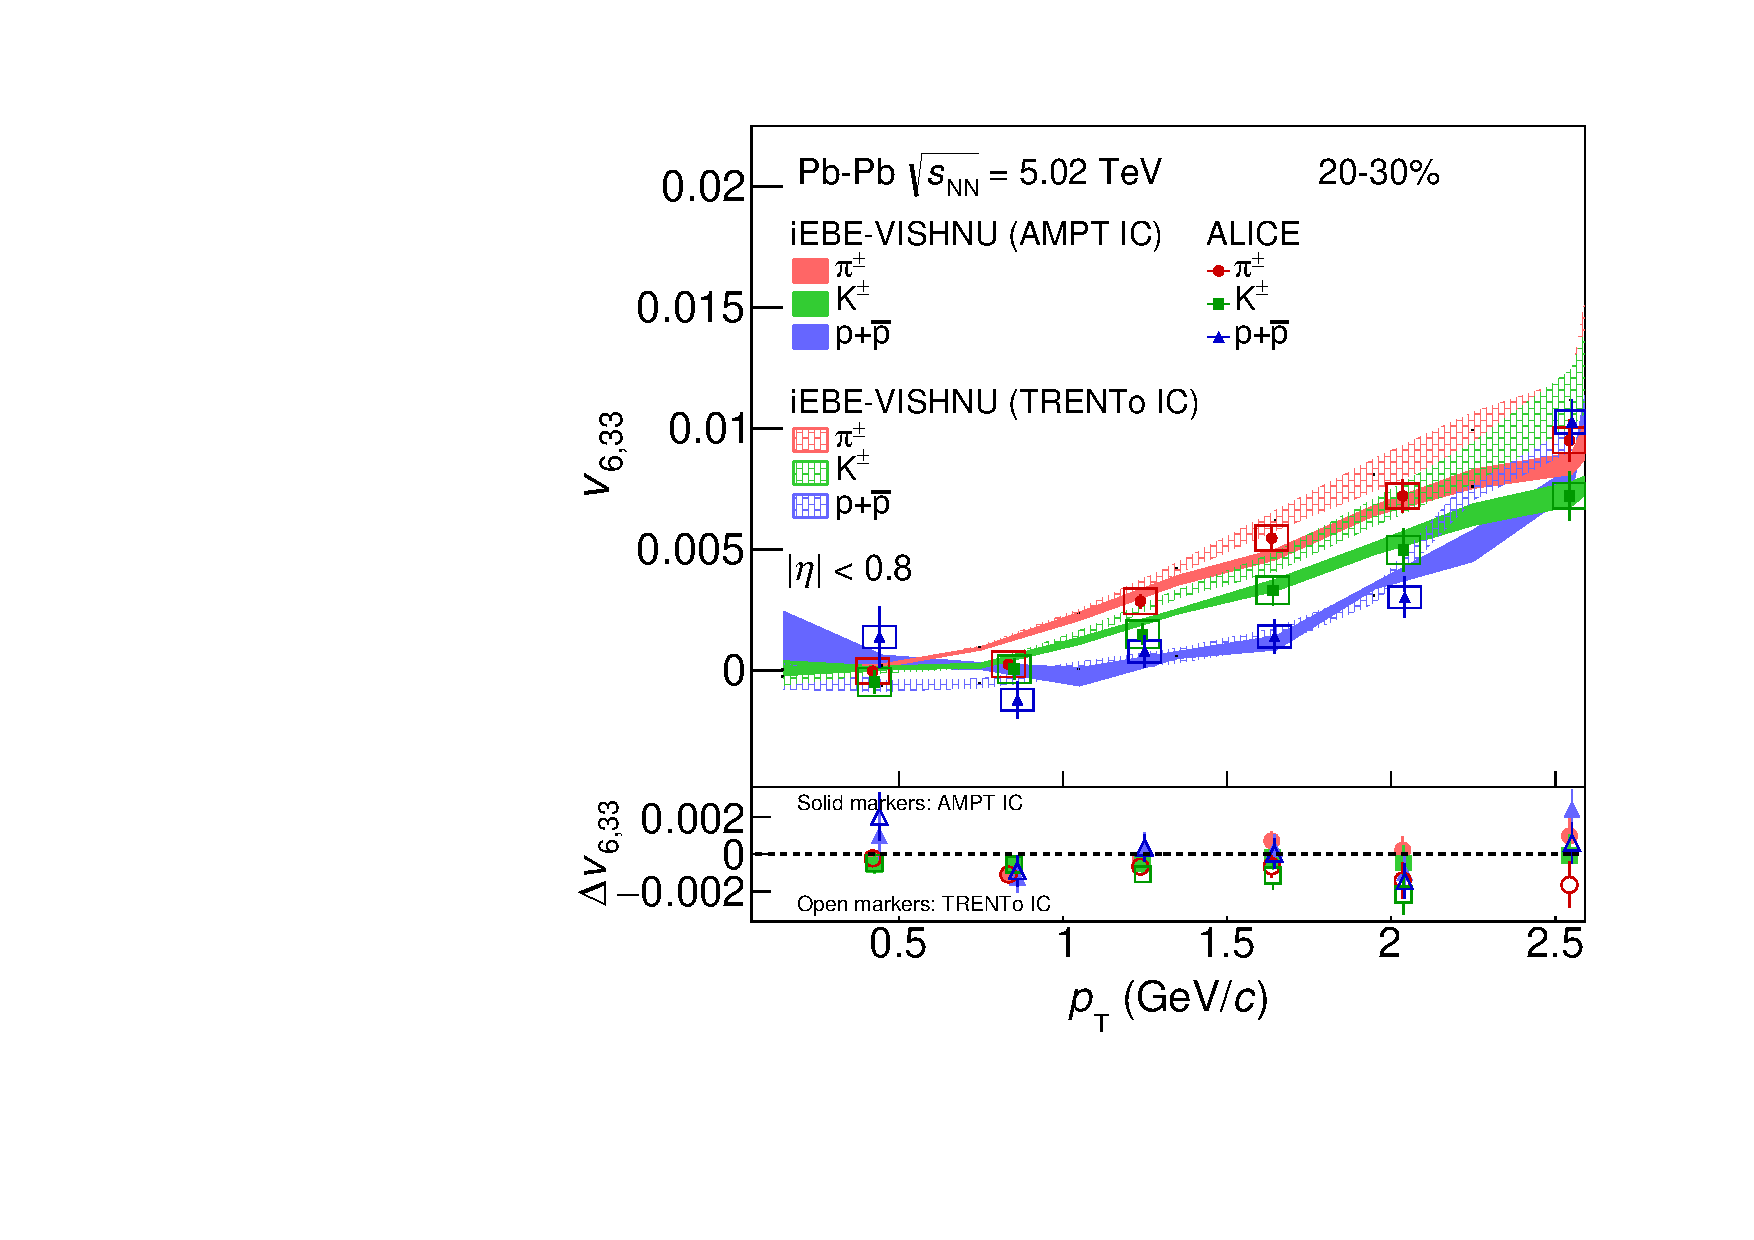
\includegraphics[scale=0.26]{figures/model/TrentoAndAMPT_v633_gap00_new_20-30_PID2.pdf}
%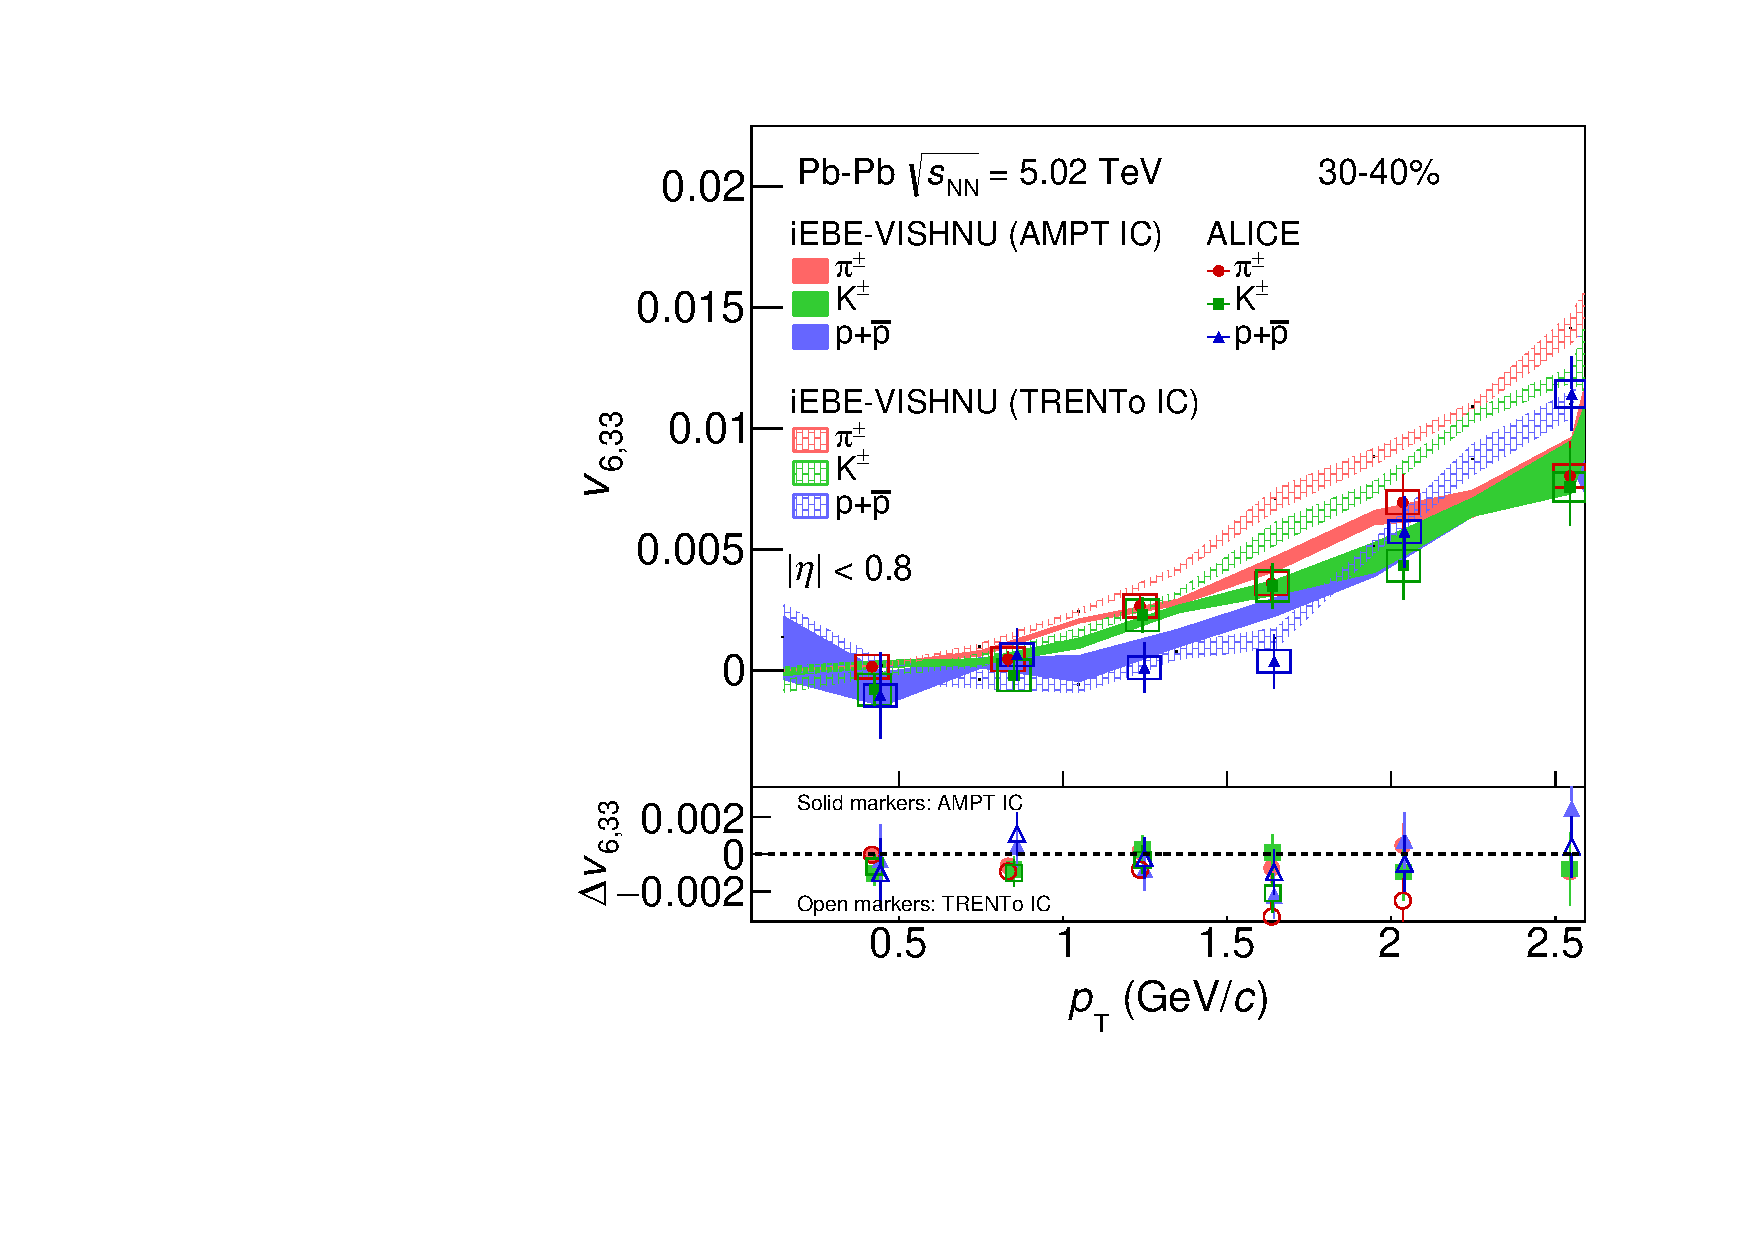
\includegraphics[scale=0.26]{figures/model/TrentoAndAMPT_v633_gap00_new_30-40_PID2.pdf}
%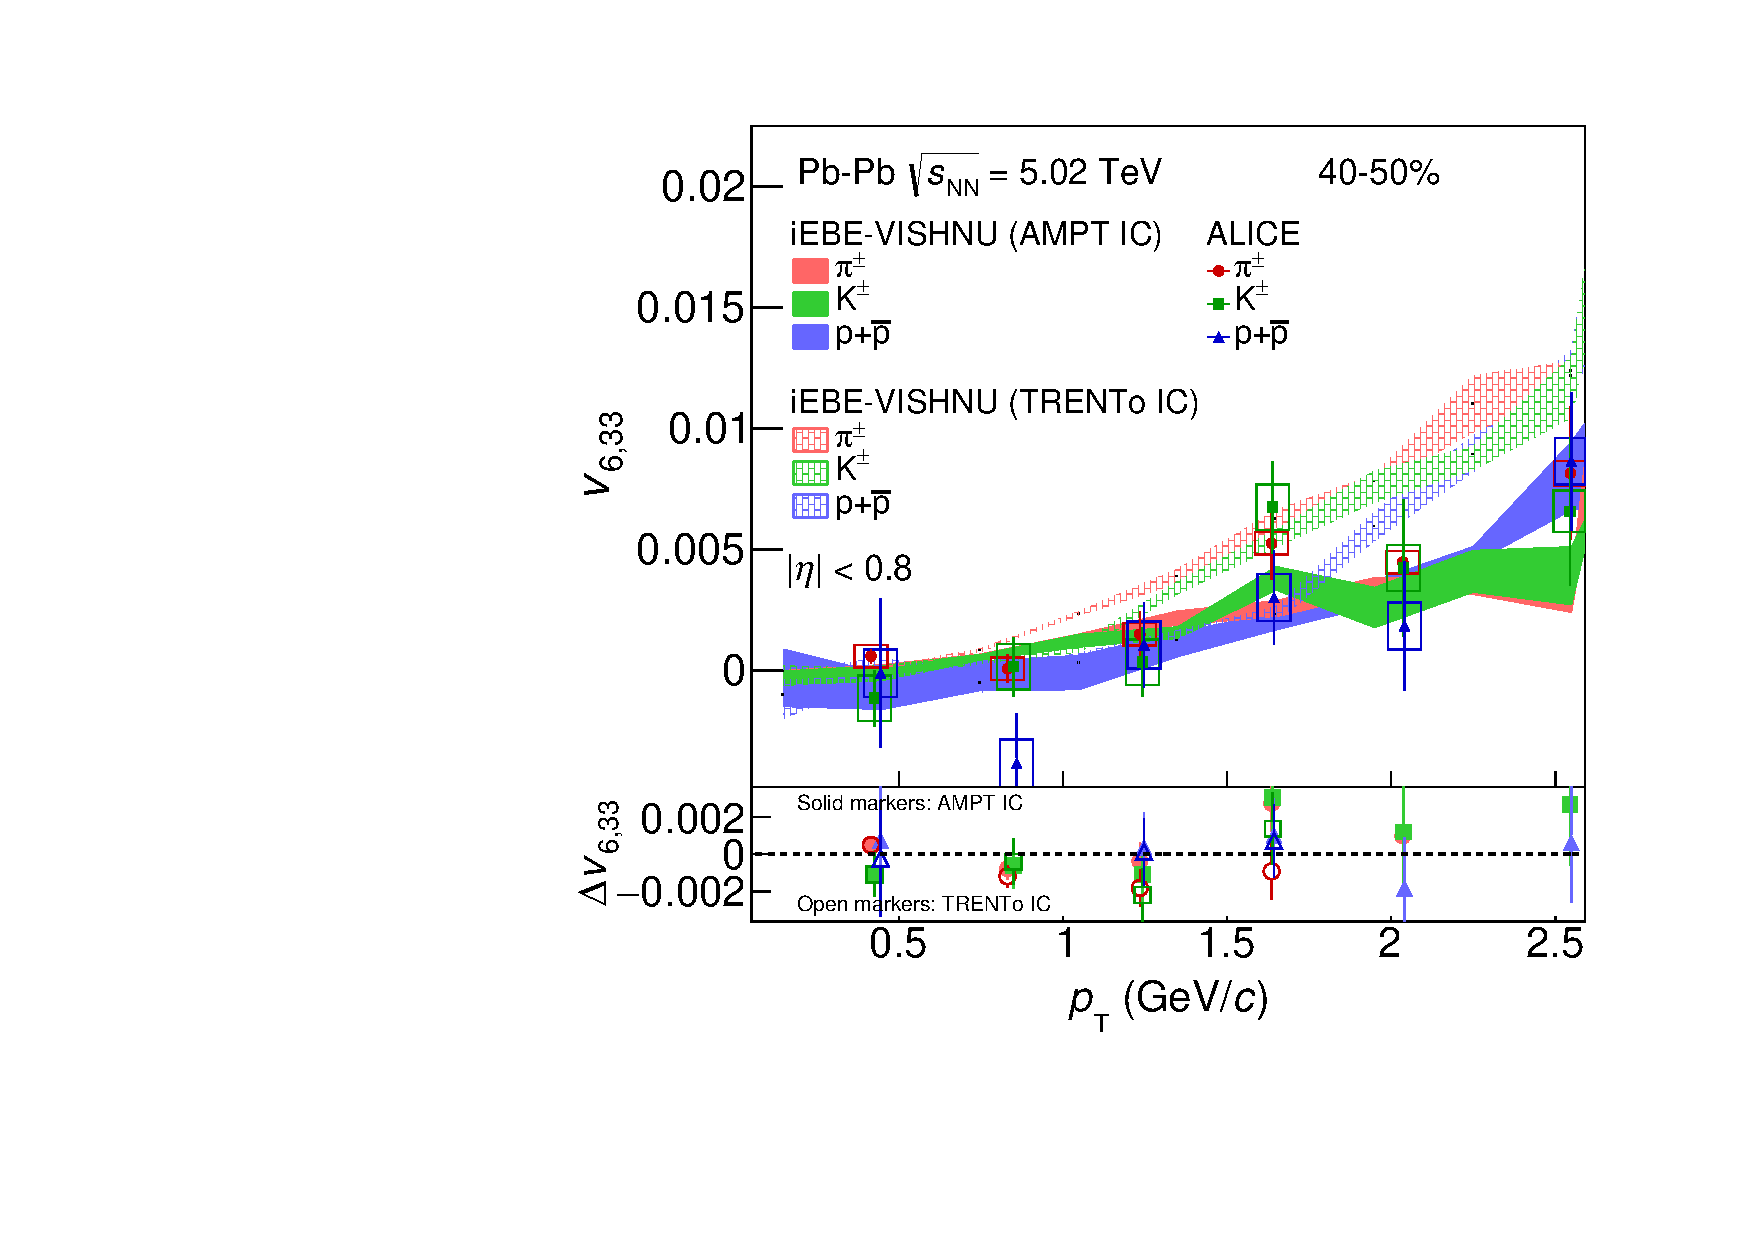
\includegraphics[scale=0.26]{figures/model/TrentoAndAMPT_v633_gap00_new_40-50_PID2.pdf}
\end{center}
\caption{The \pT-differential $v_{6,33}$ for different particle species in 10-20\% up to 40-50\% centrality intervals of Pb--Pb collisions at \sNN compared with iEBE-VISHNU hybrid models with two different sets of initial parameters: AMPT initial conditions ($\eta/s$= 0.08 and $\zeta/s$ = 0) shown in solid bands and TRENTo initial conditions ($\eta/s({\rm T})$ and $\zeta/s({\rm T})$) in hatched bands. The bottom panels show the difference between the measurements and each model.}
\label{v633_model}
\end{figure}


\begin{figure}[!htb]
\begin{center}
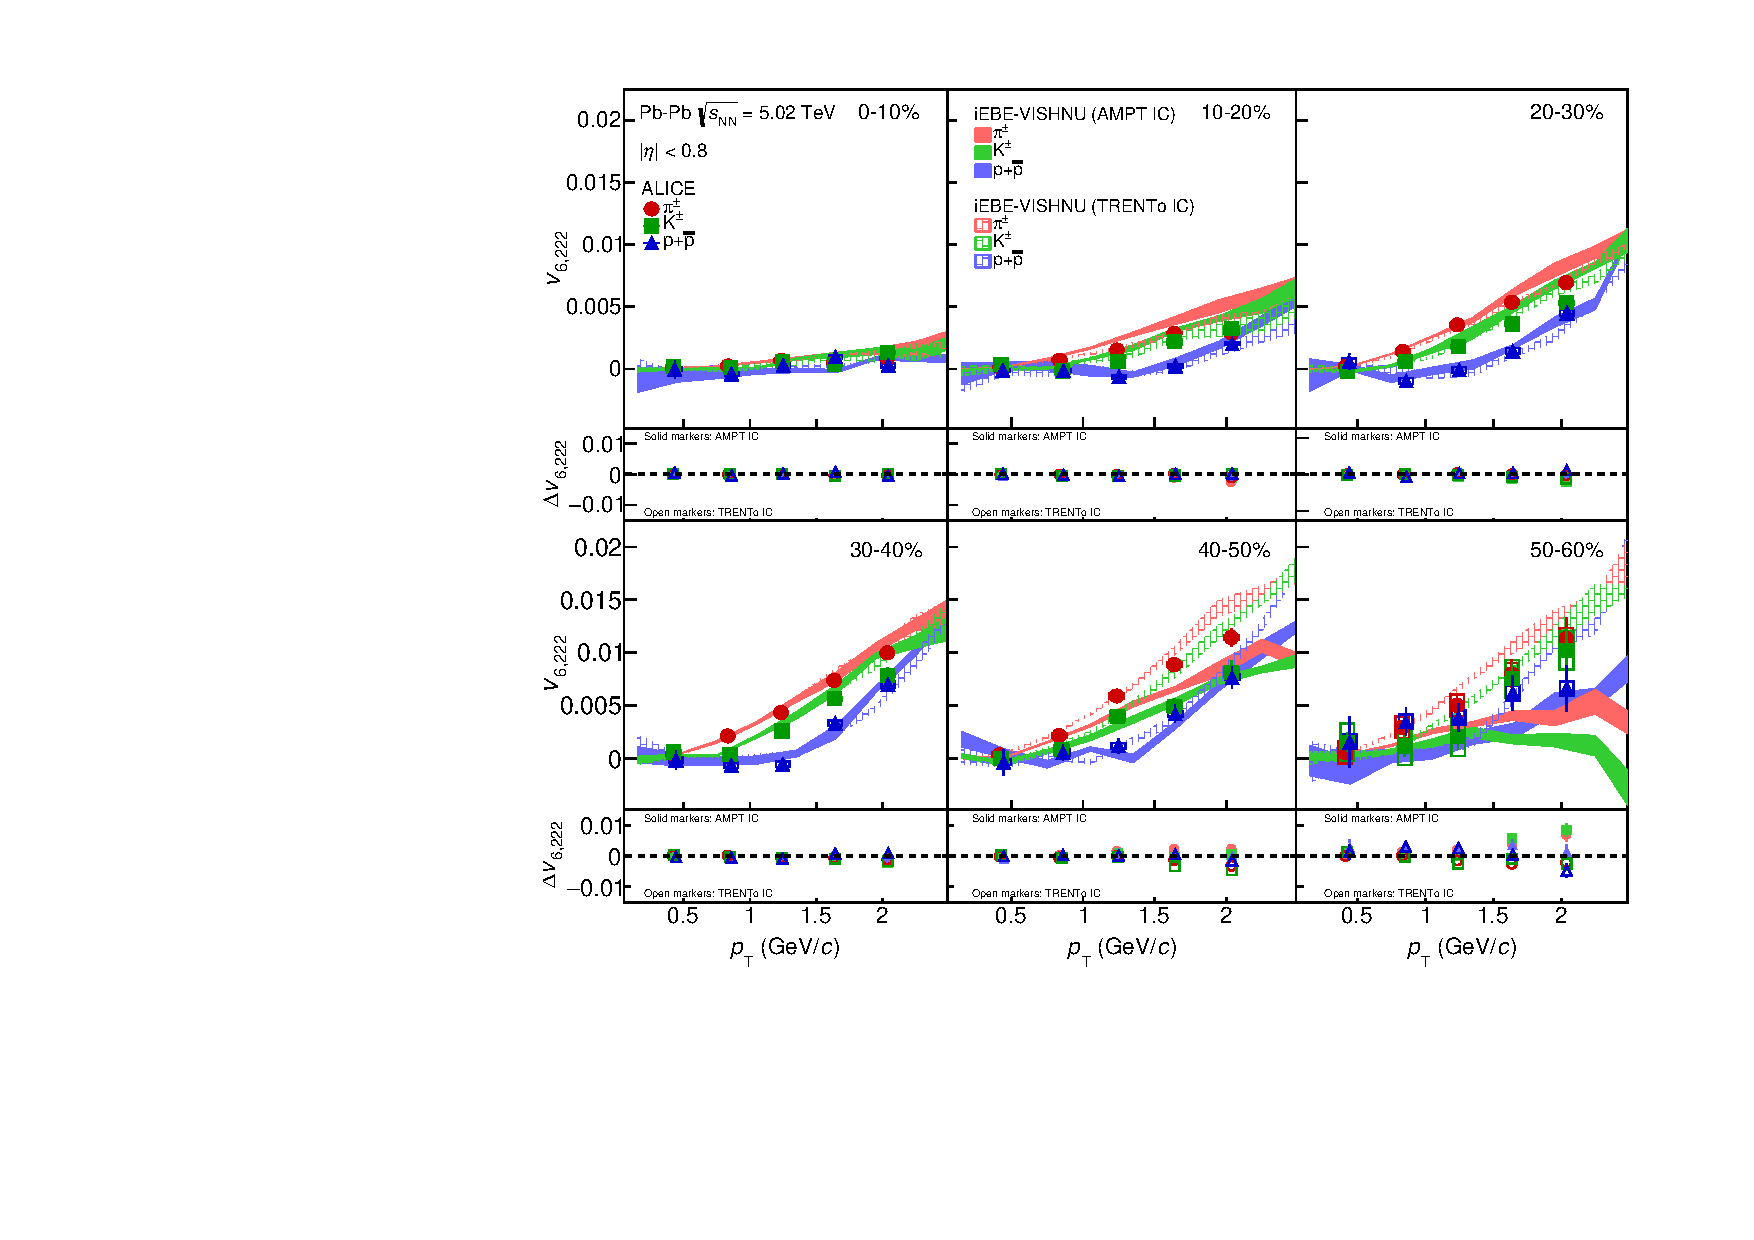
\includegraphics[scale=0.73]{figures/model/TrentoAndAMPT_v6222_gap00_PID2.pdf}
%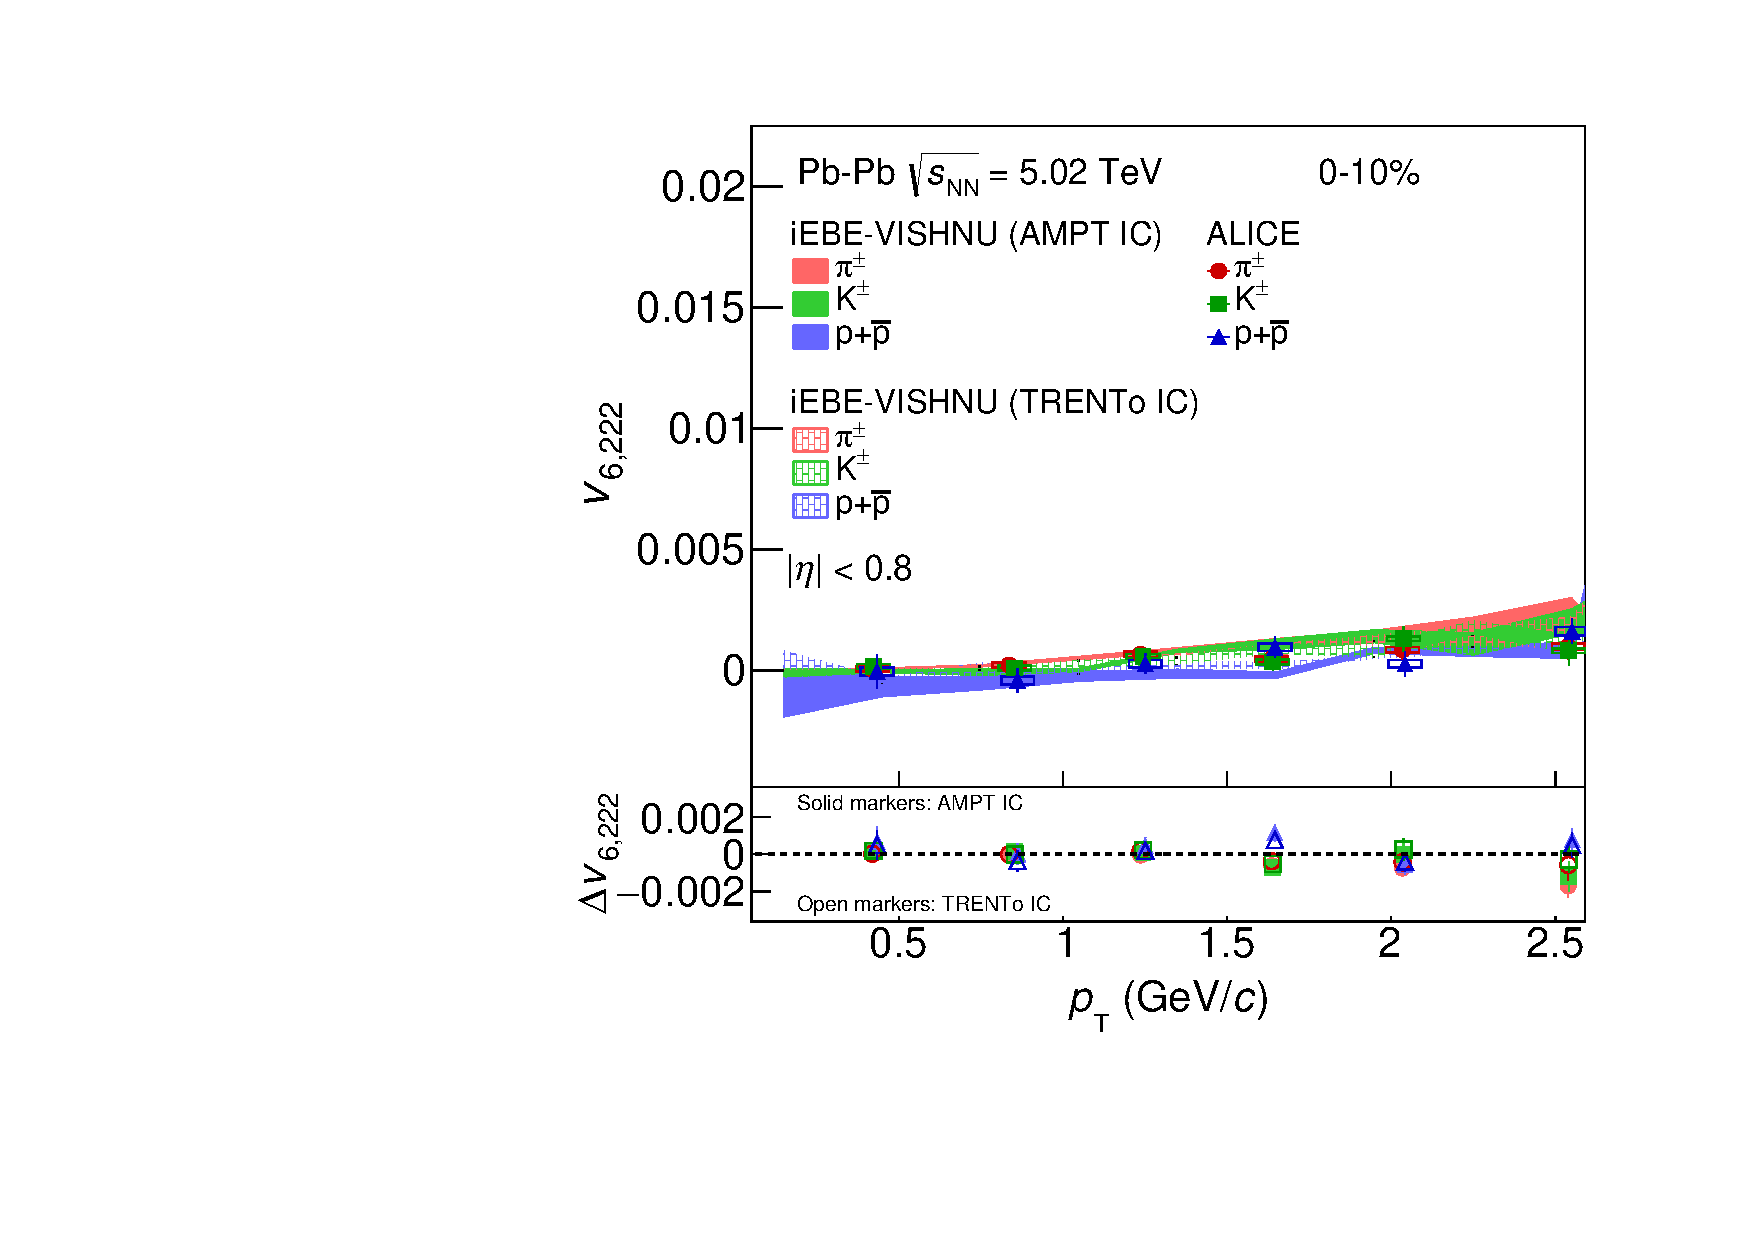
\includegraphics[scale=0.26]{figures/model/TrentoAndAMPT_v6222_gap00_new_0-10_PID2.pdf}
%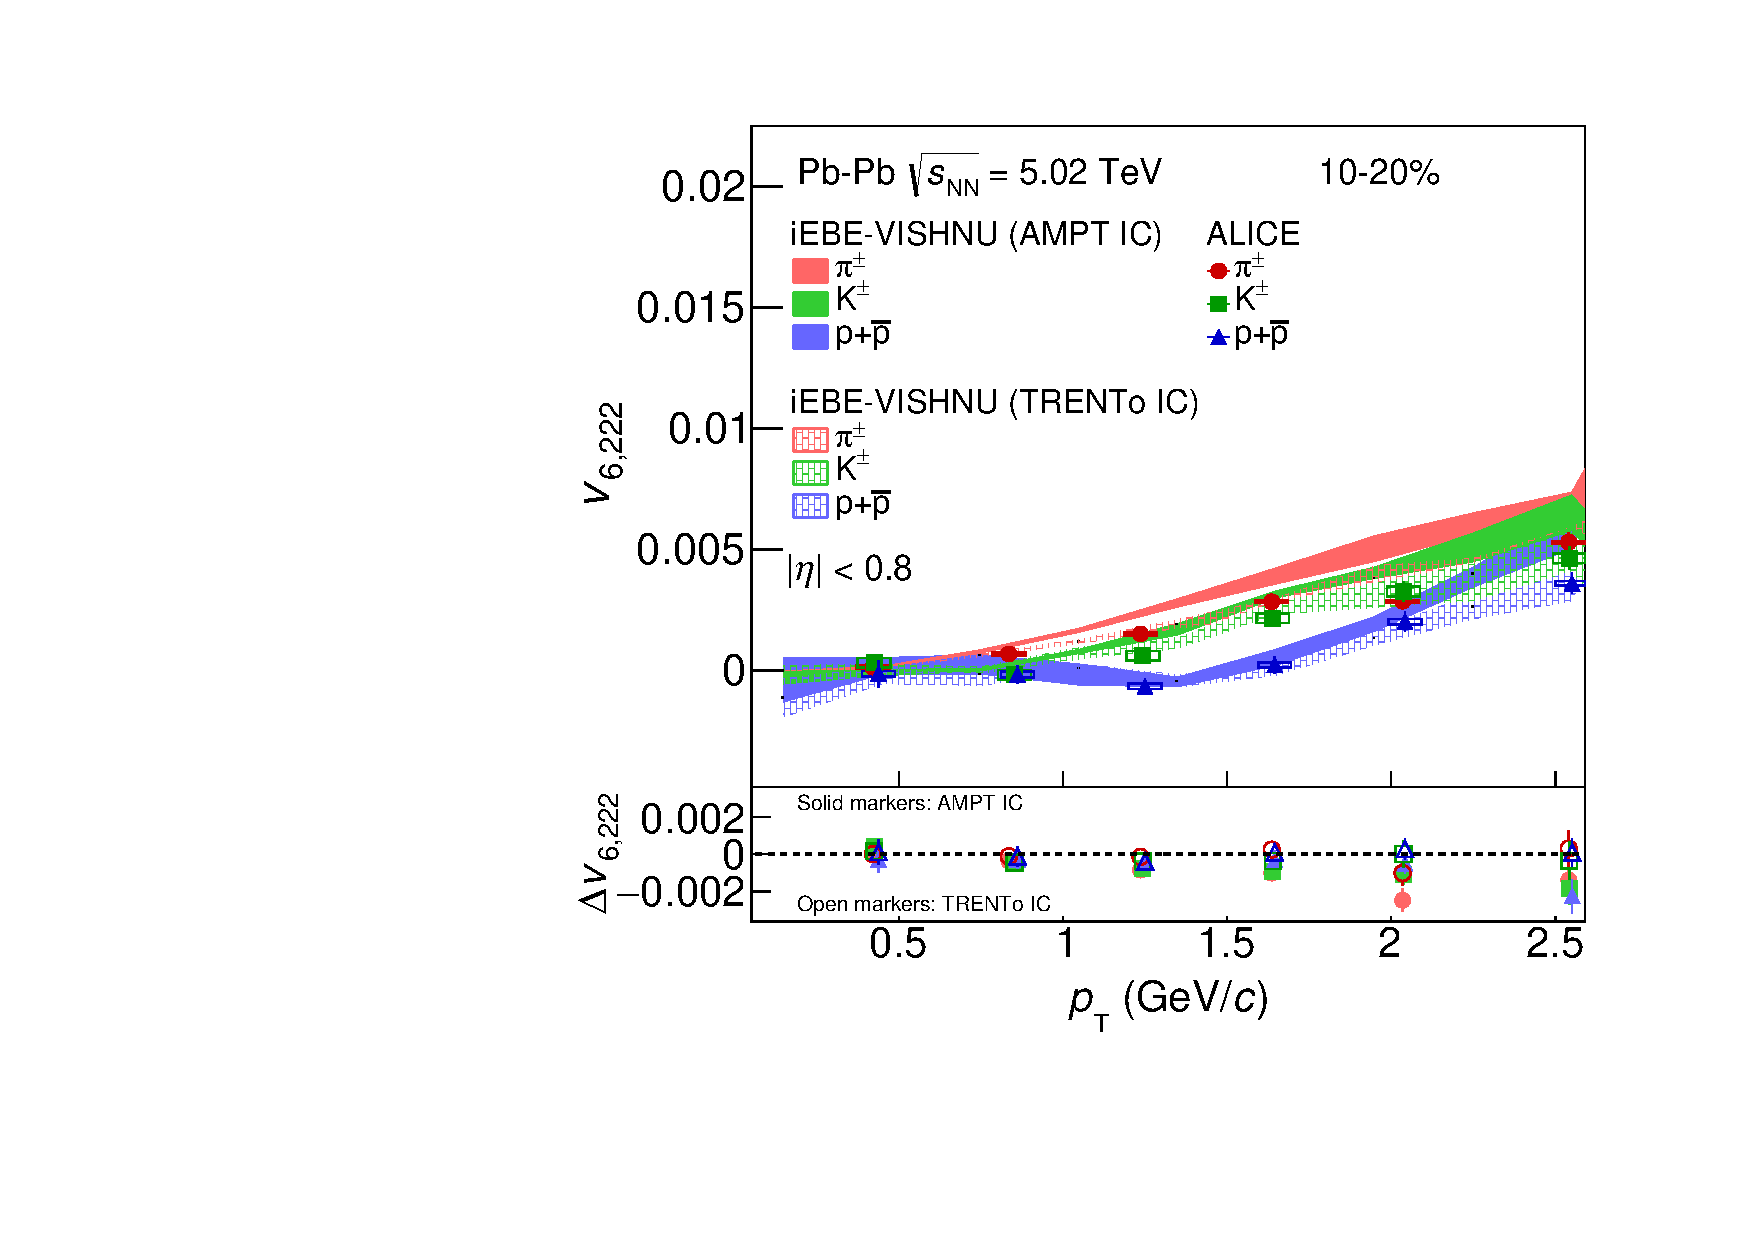
\includegraphics[scale=0.26]{figures/model/TrentoAndAMPT_v6222_gap00_new_10-20_PID2.pdf}
%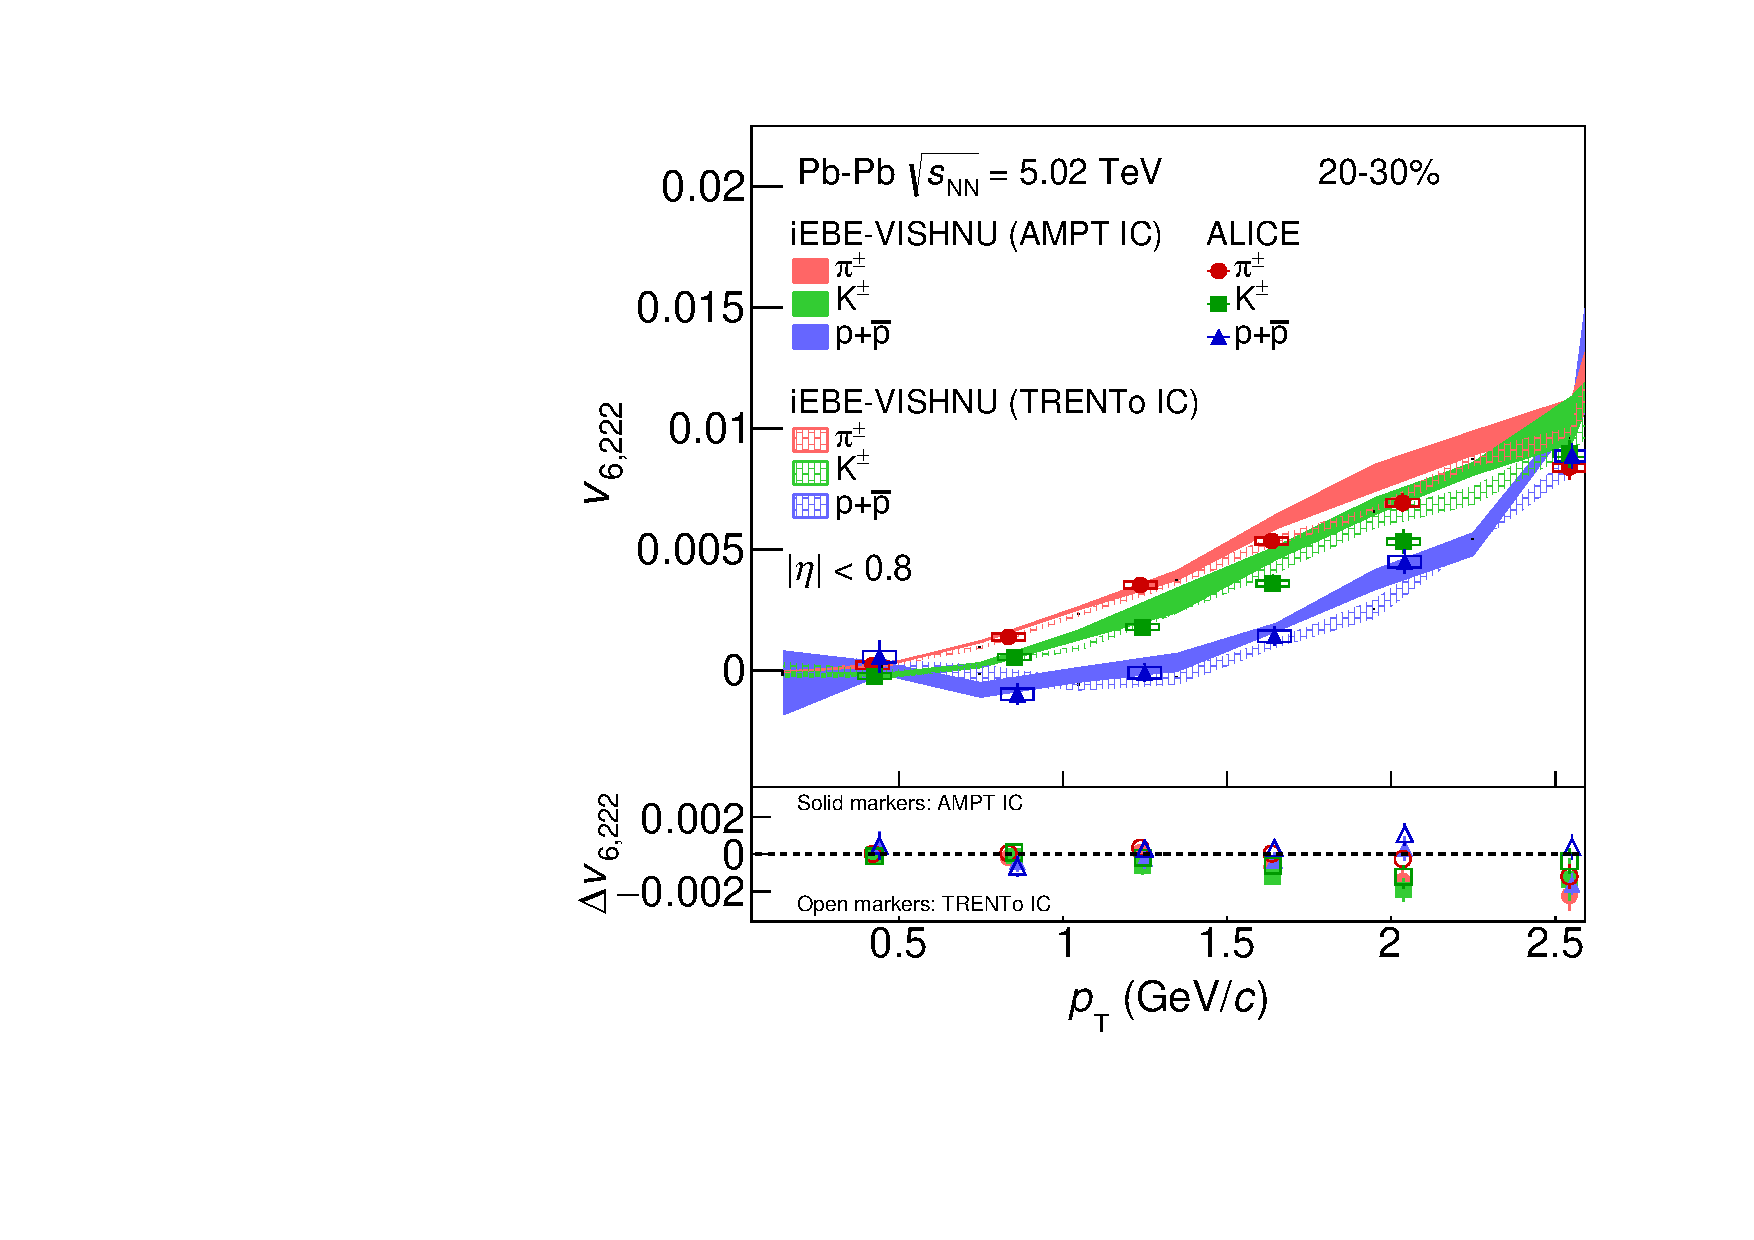
\includegraphics[scale=0.26]{figures/model/TrentoAndAMPT_v6222_gap00_new_20-30_PID2.pdf}
%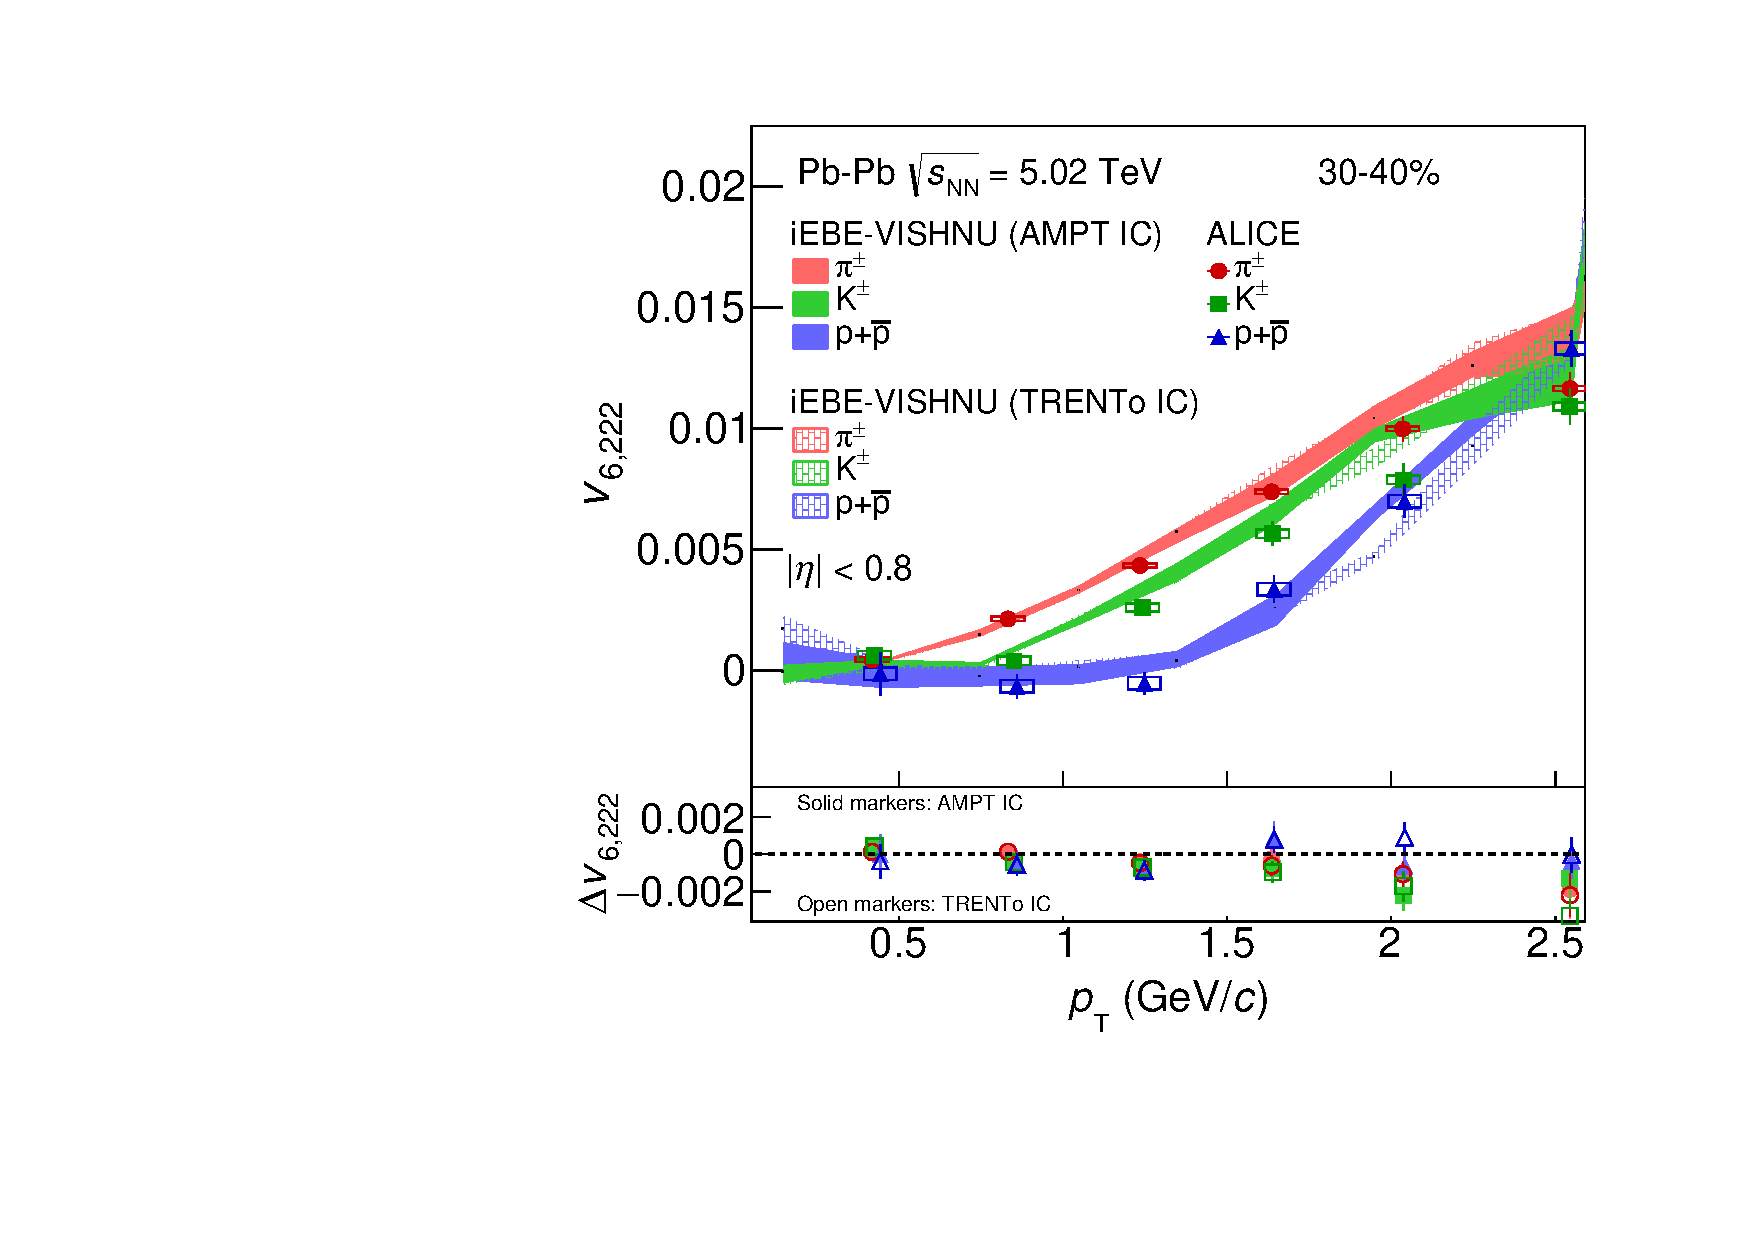
\includegraphics[scale=0.26]{figures/model/TrentoAndAMPT_v6222_gap00_new_30-40_PID2.pdf}
%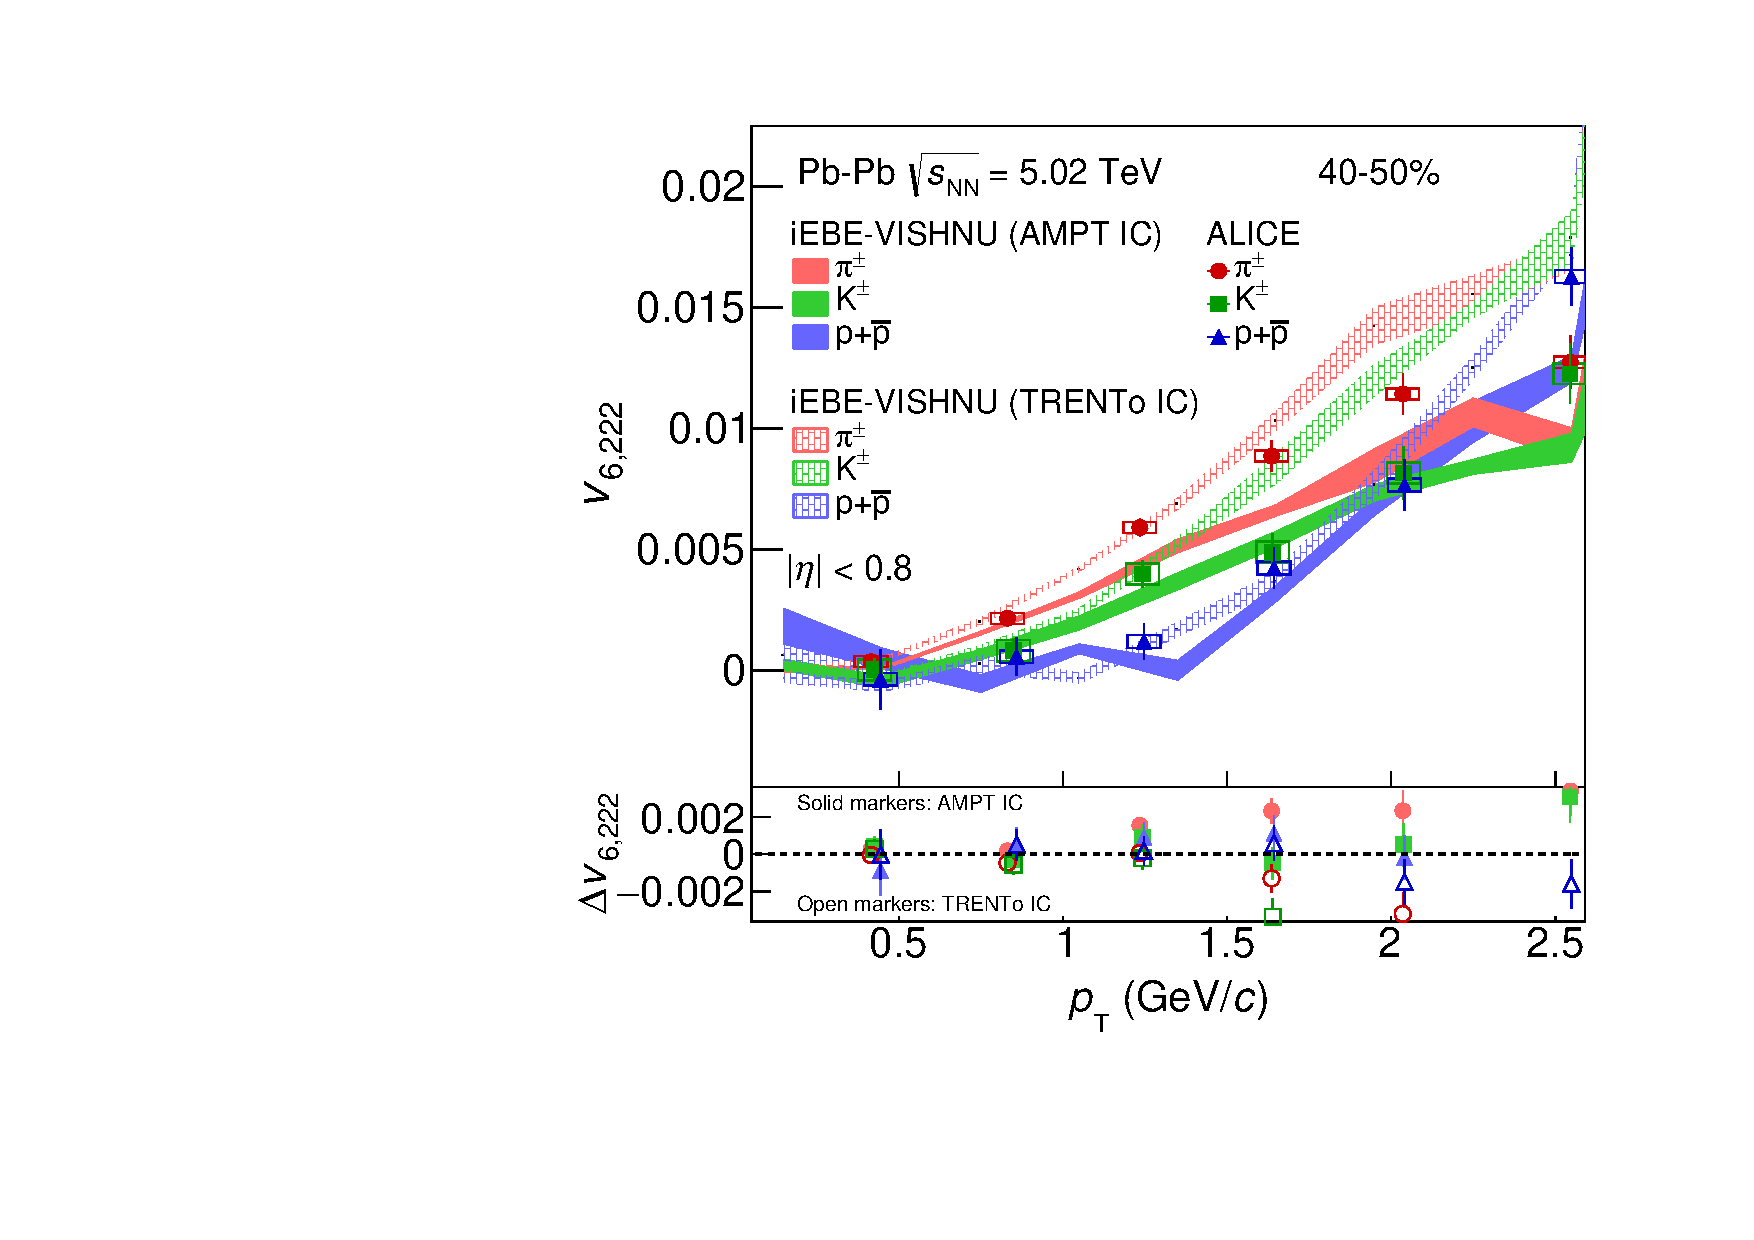
\includegraphics[scale=0.26]{figures/model/TrentoAndAMPT_v6222_gap00_new_40-50_PID2.pdf}
%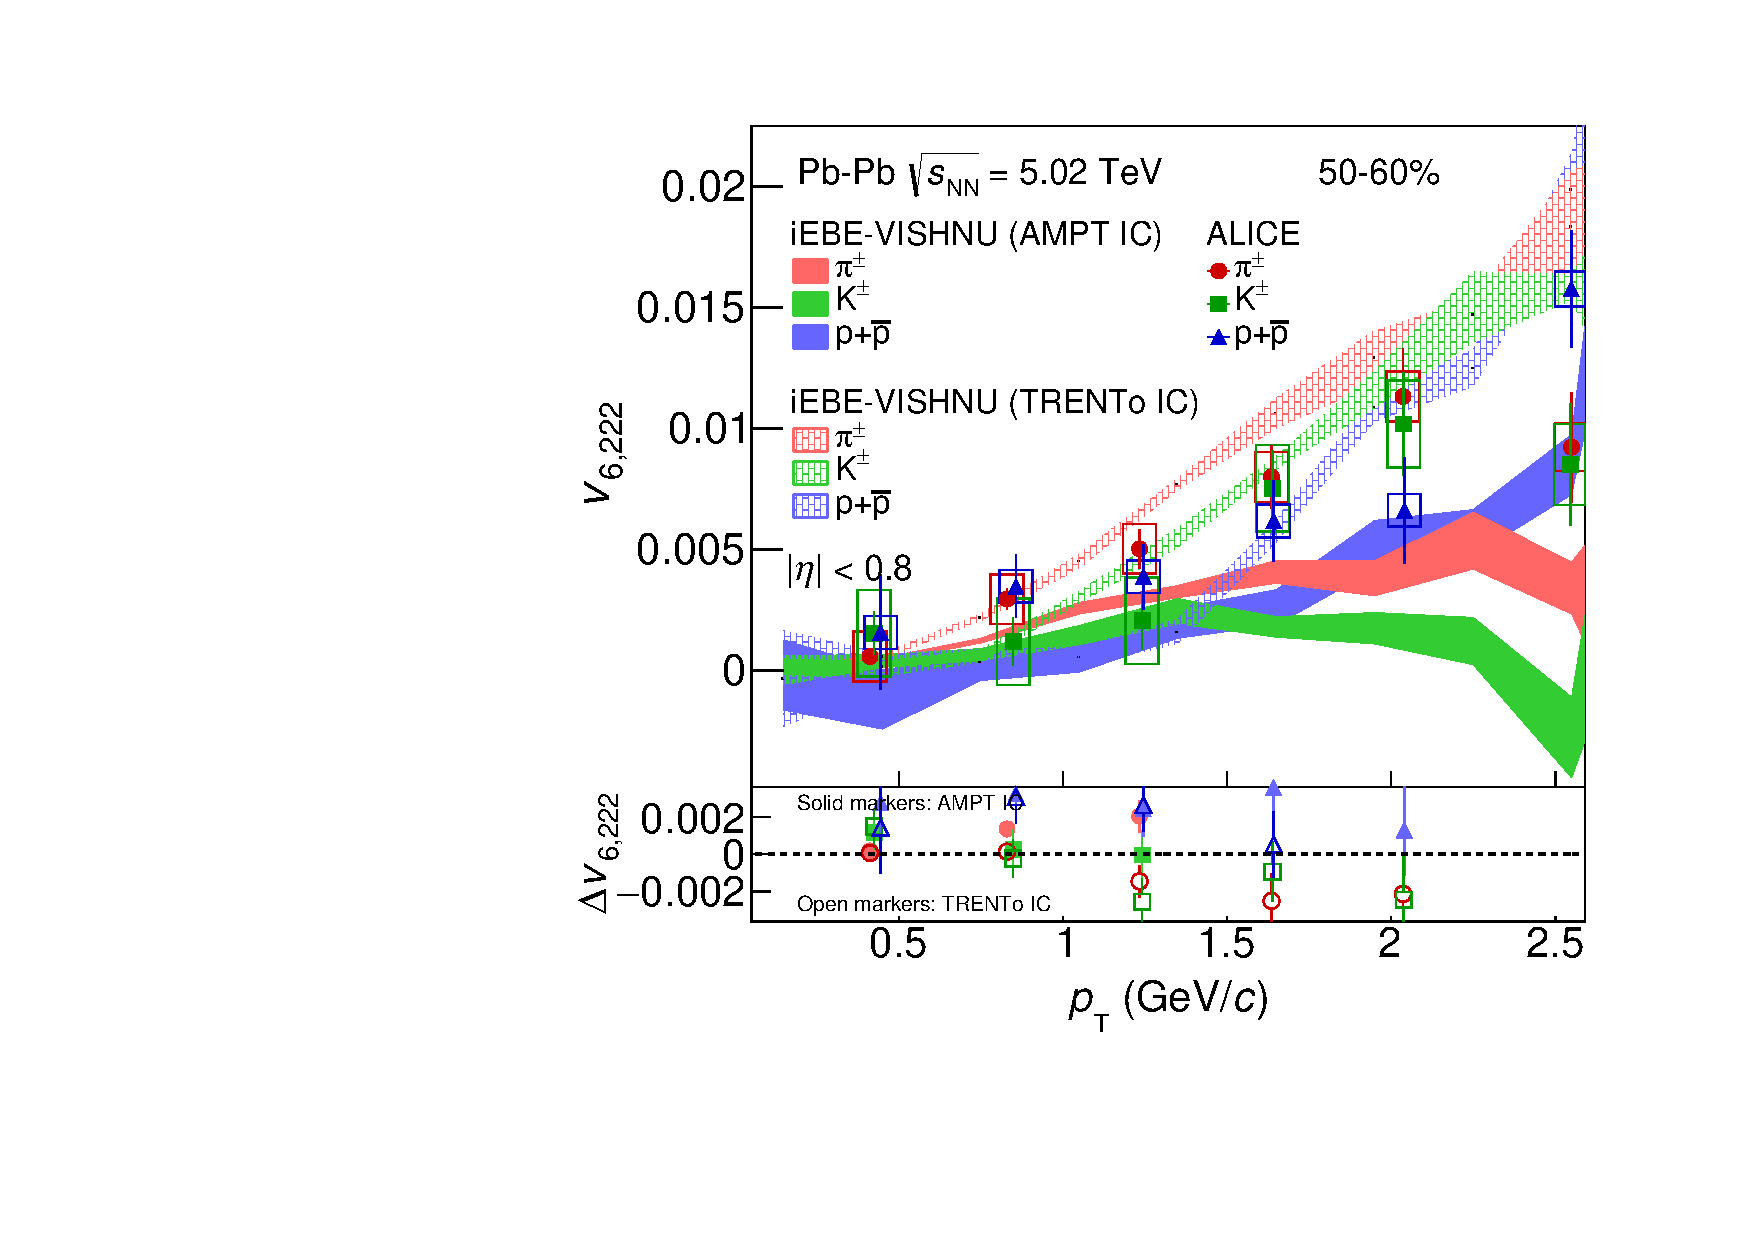
\includegraphics[scale=0.26]{figures/model/TrentoAndAMPT_v6222_gap00_new_50-60_PID2.pdf}
\end{center}
\caption{The \pT-differential $v_{6,222}$ for different particle species in 10-20\% up to 50-60\% centrality intervals of Pb--Pb collisions at \sNN compared with iEBE-VISHNU hybrid models with two different sets of initial parameters: AMPT initial conditions ($\eta/s$= 0.08 and $\zeta/s$ = 0) shown in solid bands and TRENTo initial conditions ($\eta/s({\rm T})$ and $\zeta/s({\rm T})$) in hatched bands. The bottom panels show the difference between the measurements and each model.}
\label{v6222_model}
\end{figure}



\newpage